\chapter{Neutrino Lifetime Fit Supplementary Plots}

\section{1/3 Dataset}
\label{third_observables}

In the following sections are both the observables at the fit minimum and the observables for a more traditional no-decay scenario with $k_2$ fixed to infinity. 

\subsection{Fit Minimum}

Shown in \Cref{fig:third_d2o_obs,fig:third_salt_obs,fig:third_ncd_pmt_obs} are the observable distributions for the neutrino lifetime fit to the 1/3 dataset as described in \Cref{third}.

\begin{figure}
\centering
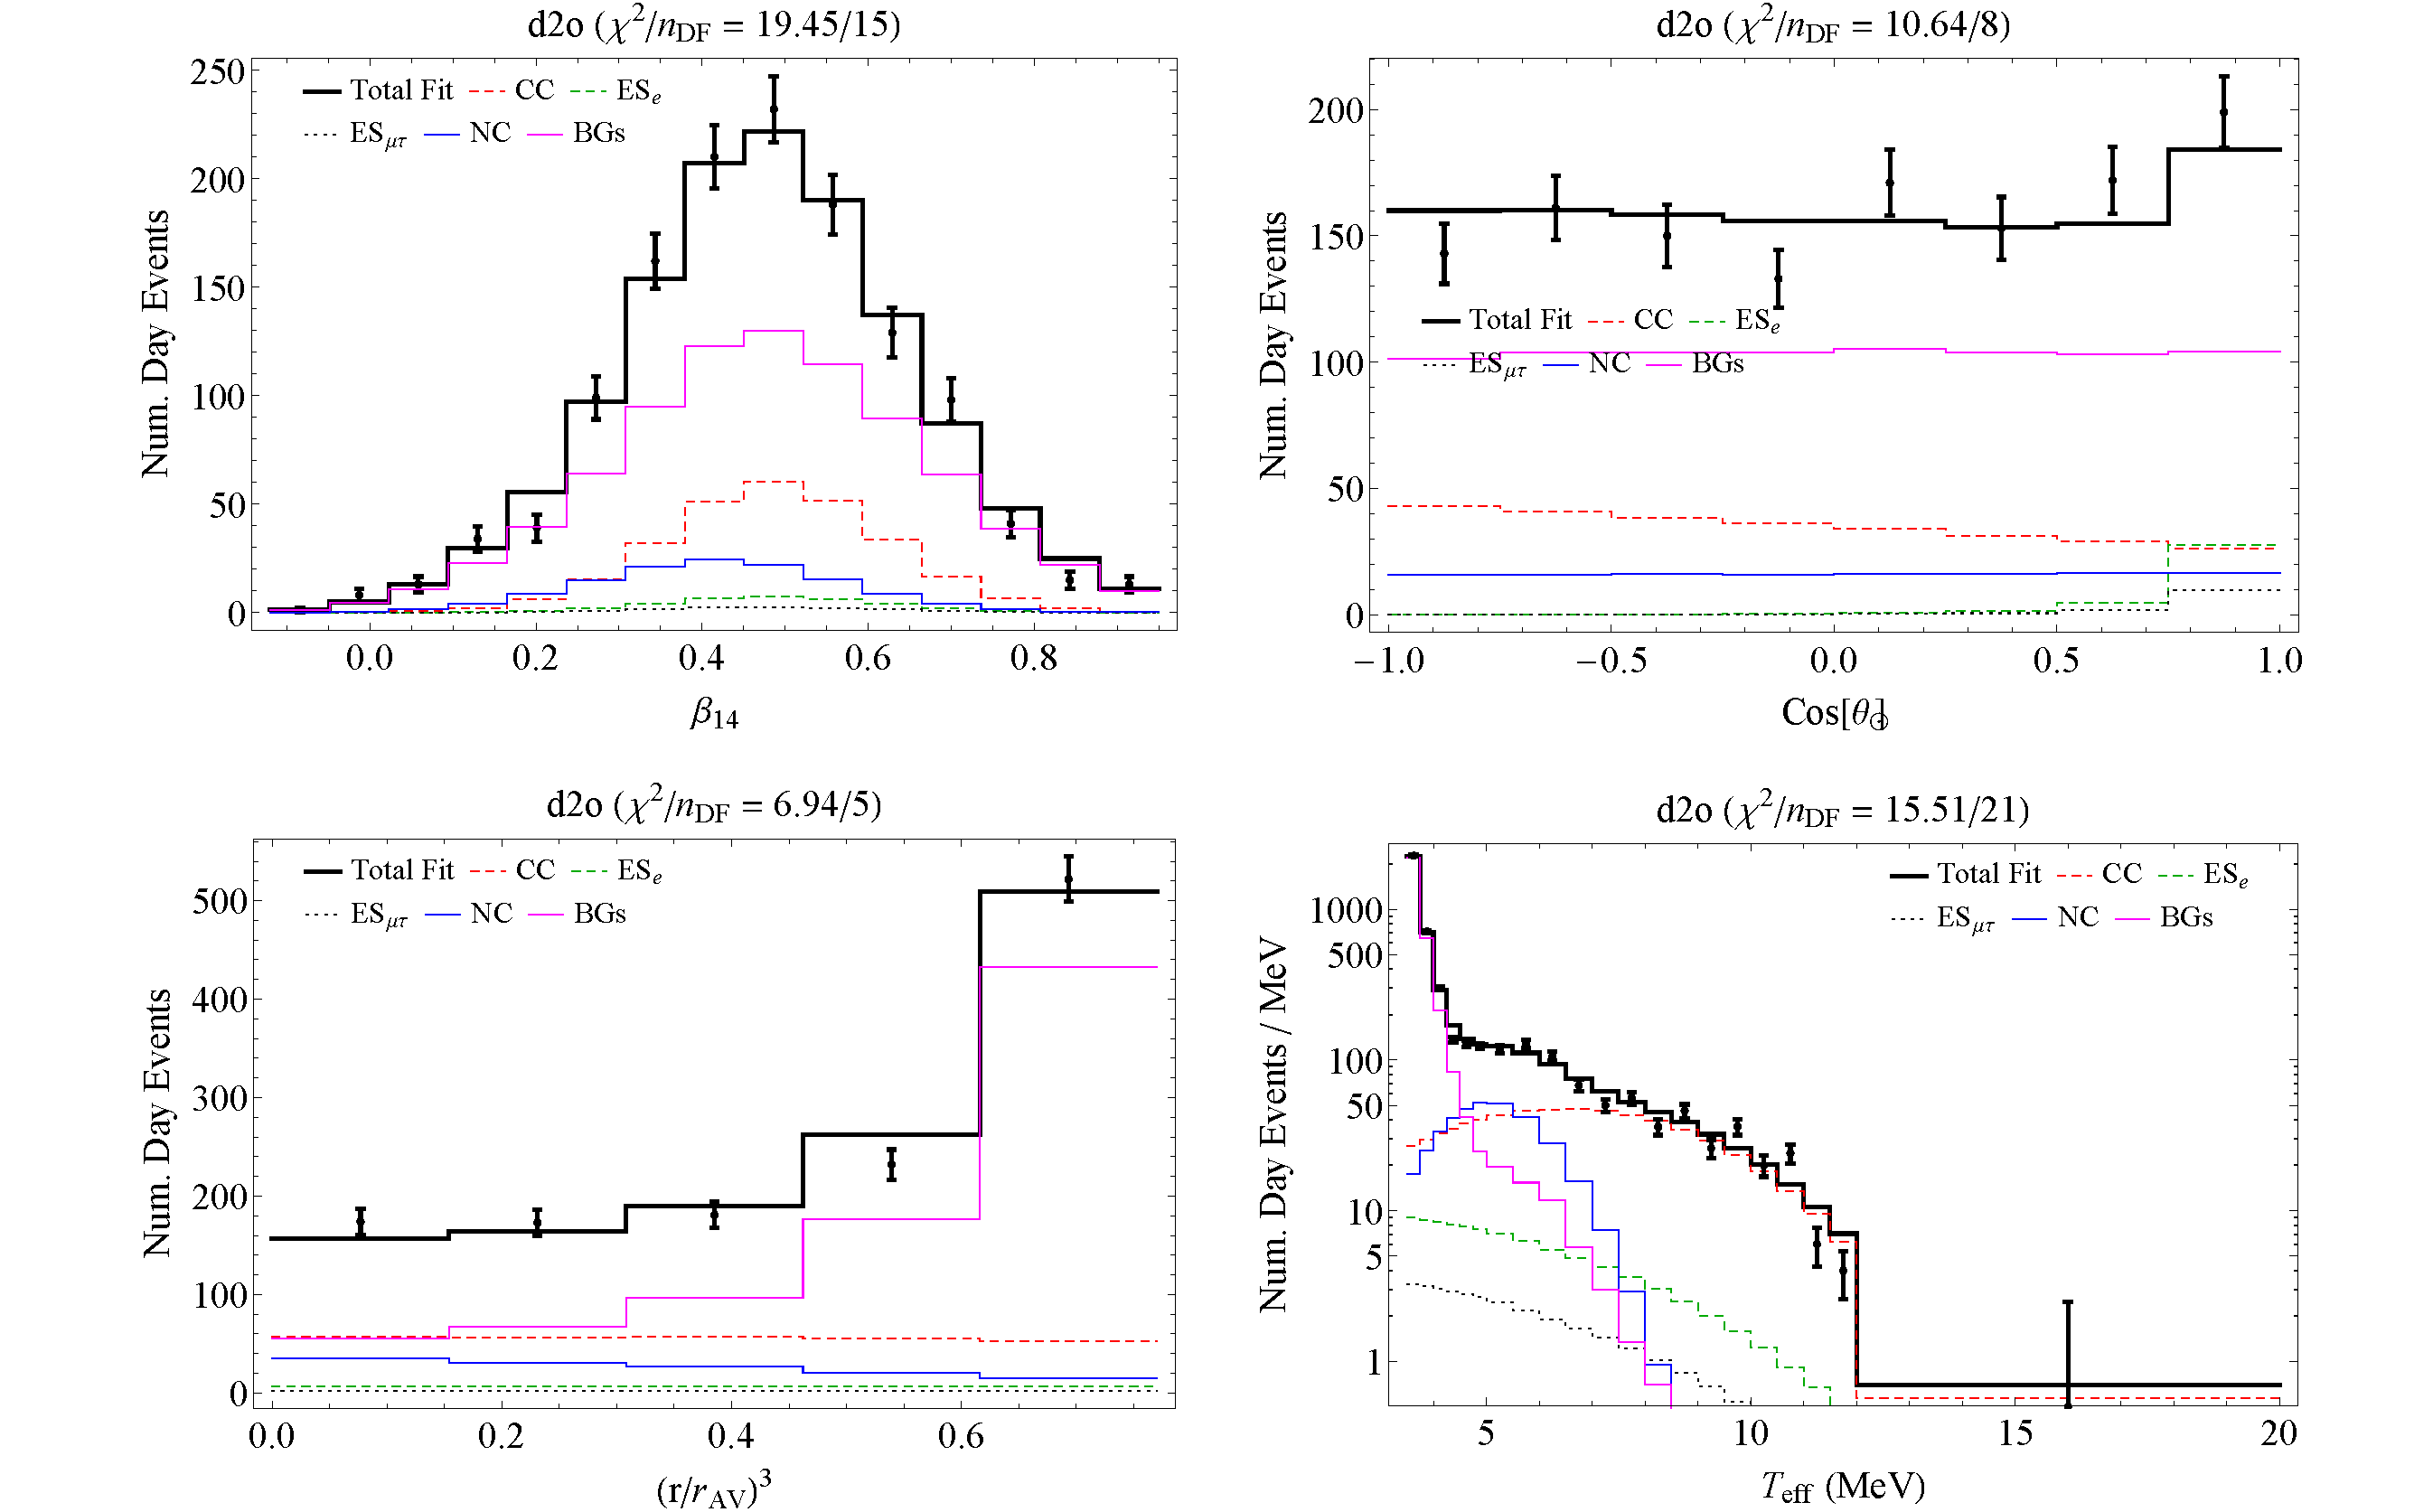
\includegraphics[width=0.95\columnwidth]{third_d2o_day}
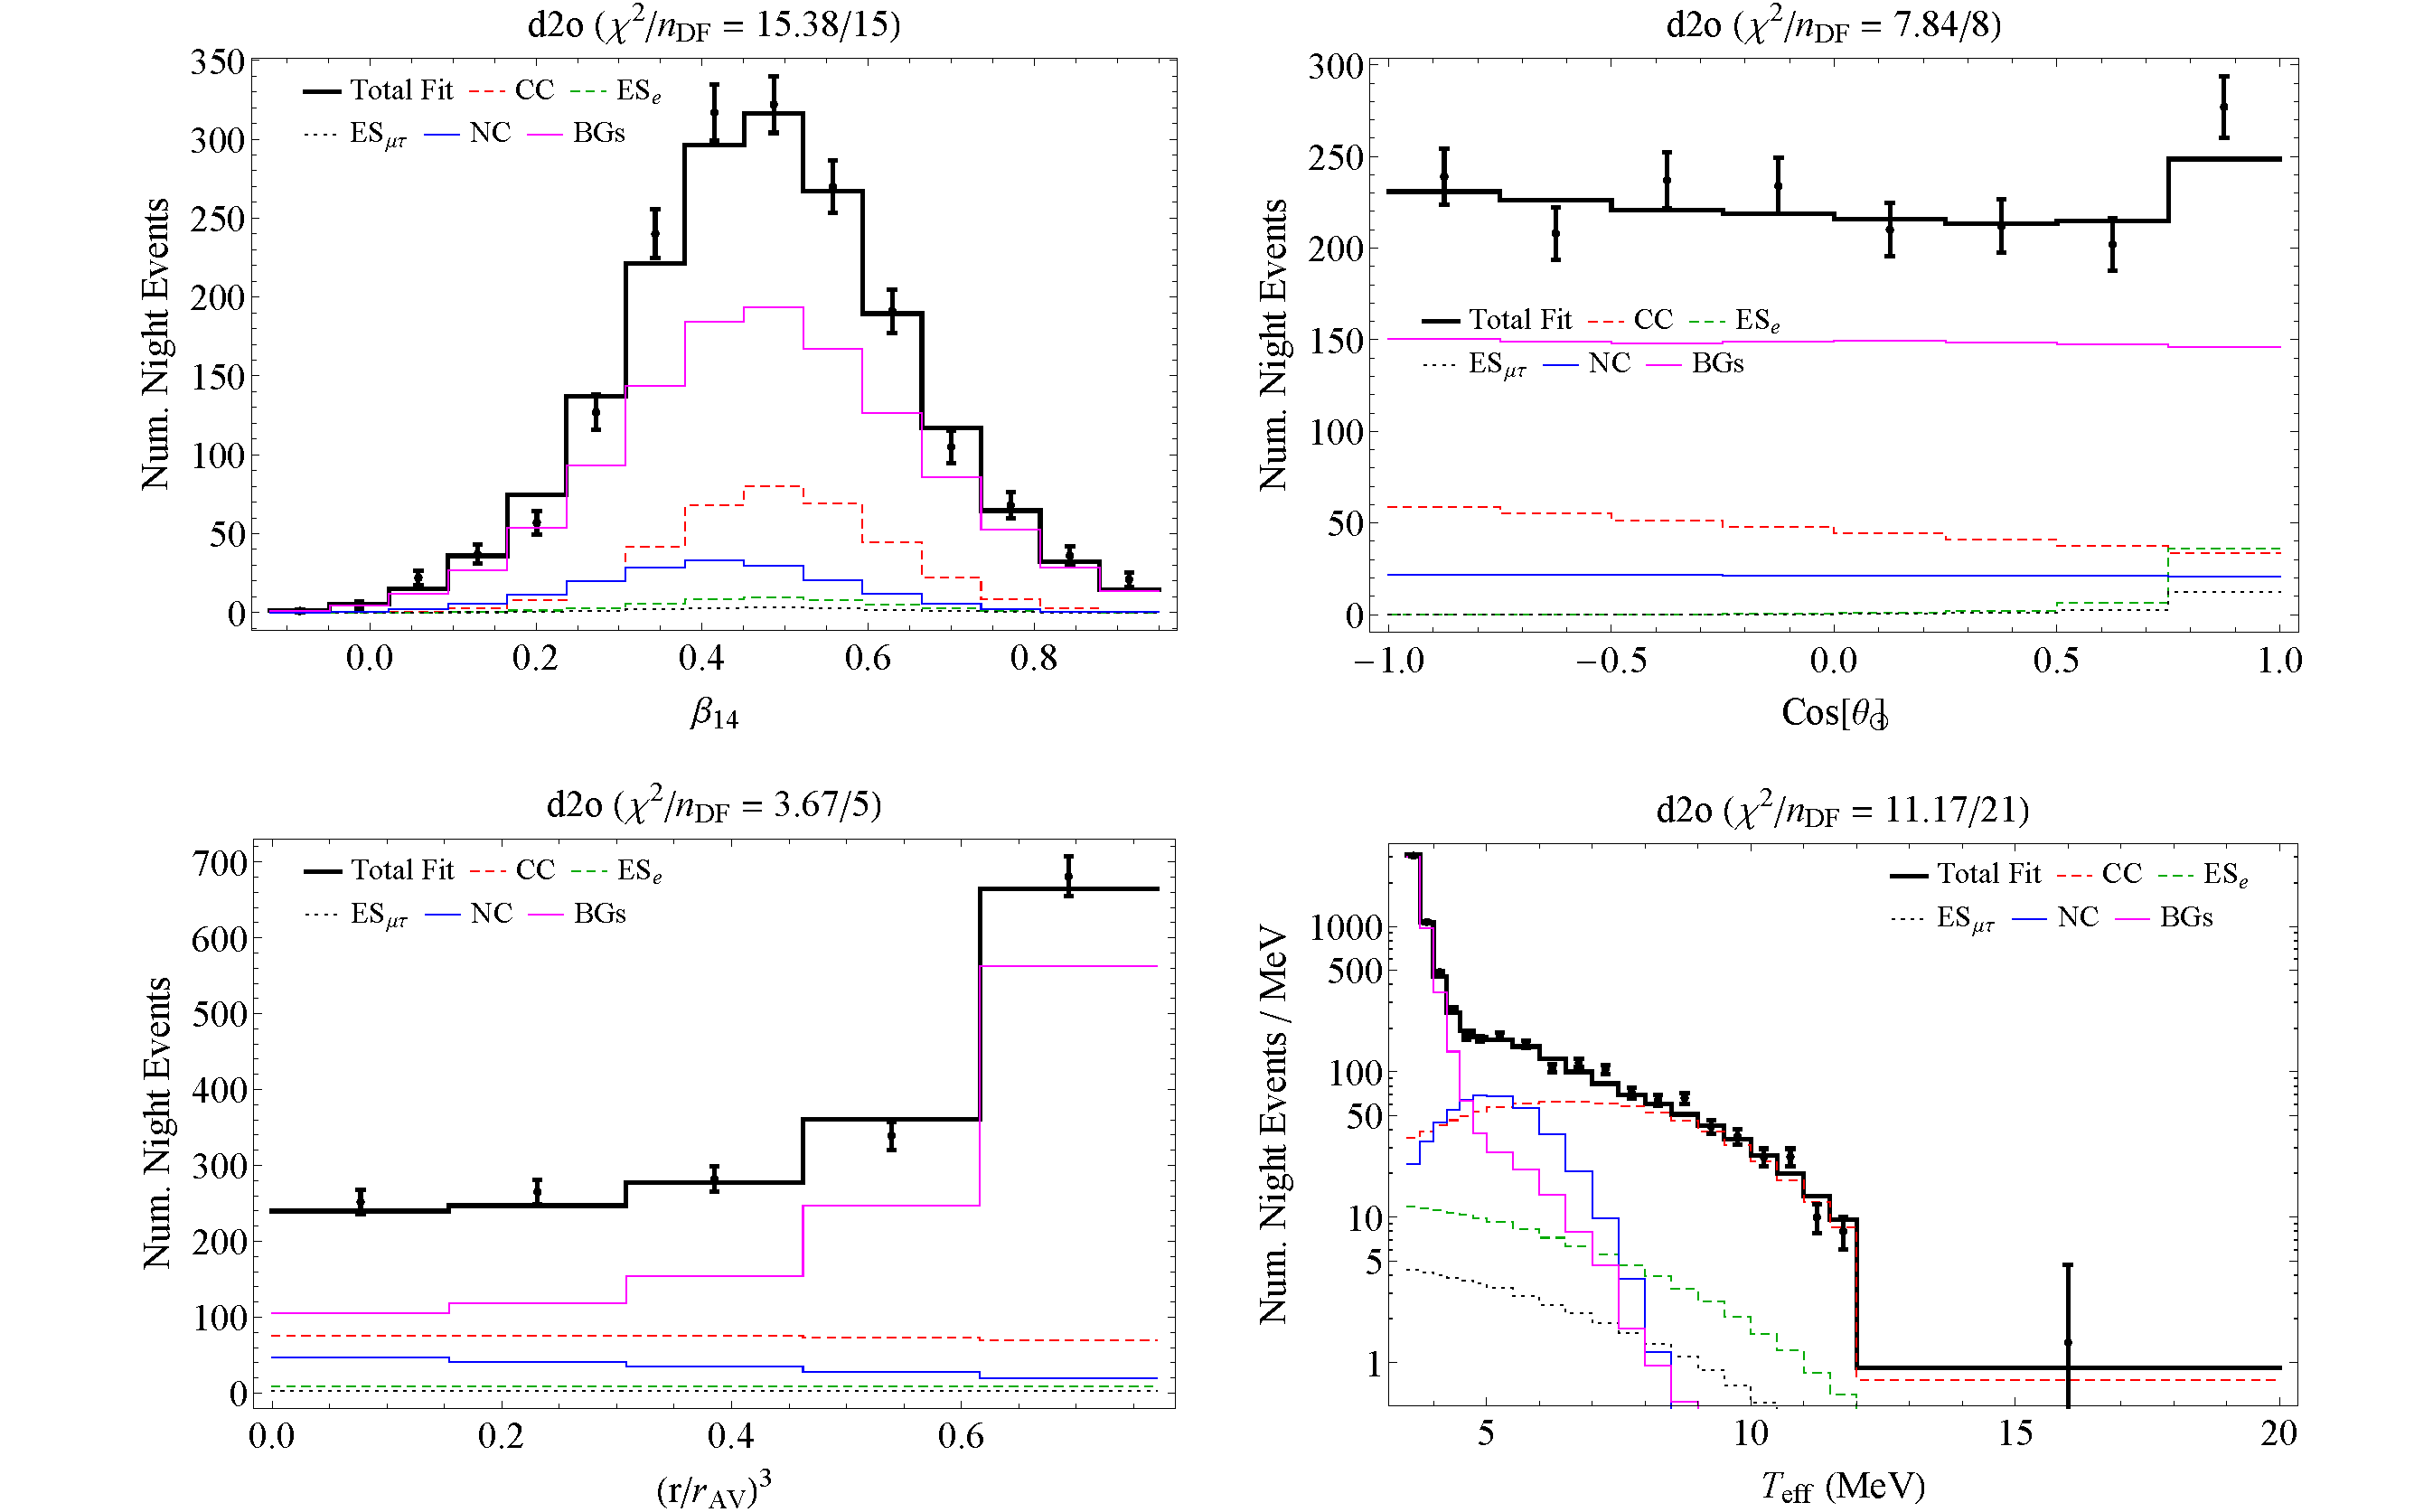
\includegraphics[width=0.95\columnwidth]{third_d2o_night}
\caption{\label{fig:third_d2o_obs}Observable distributions for Phase I for the 1/3 dataset fit.}
\end{figure}
\begin{figure}
\centering
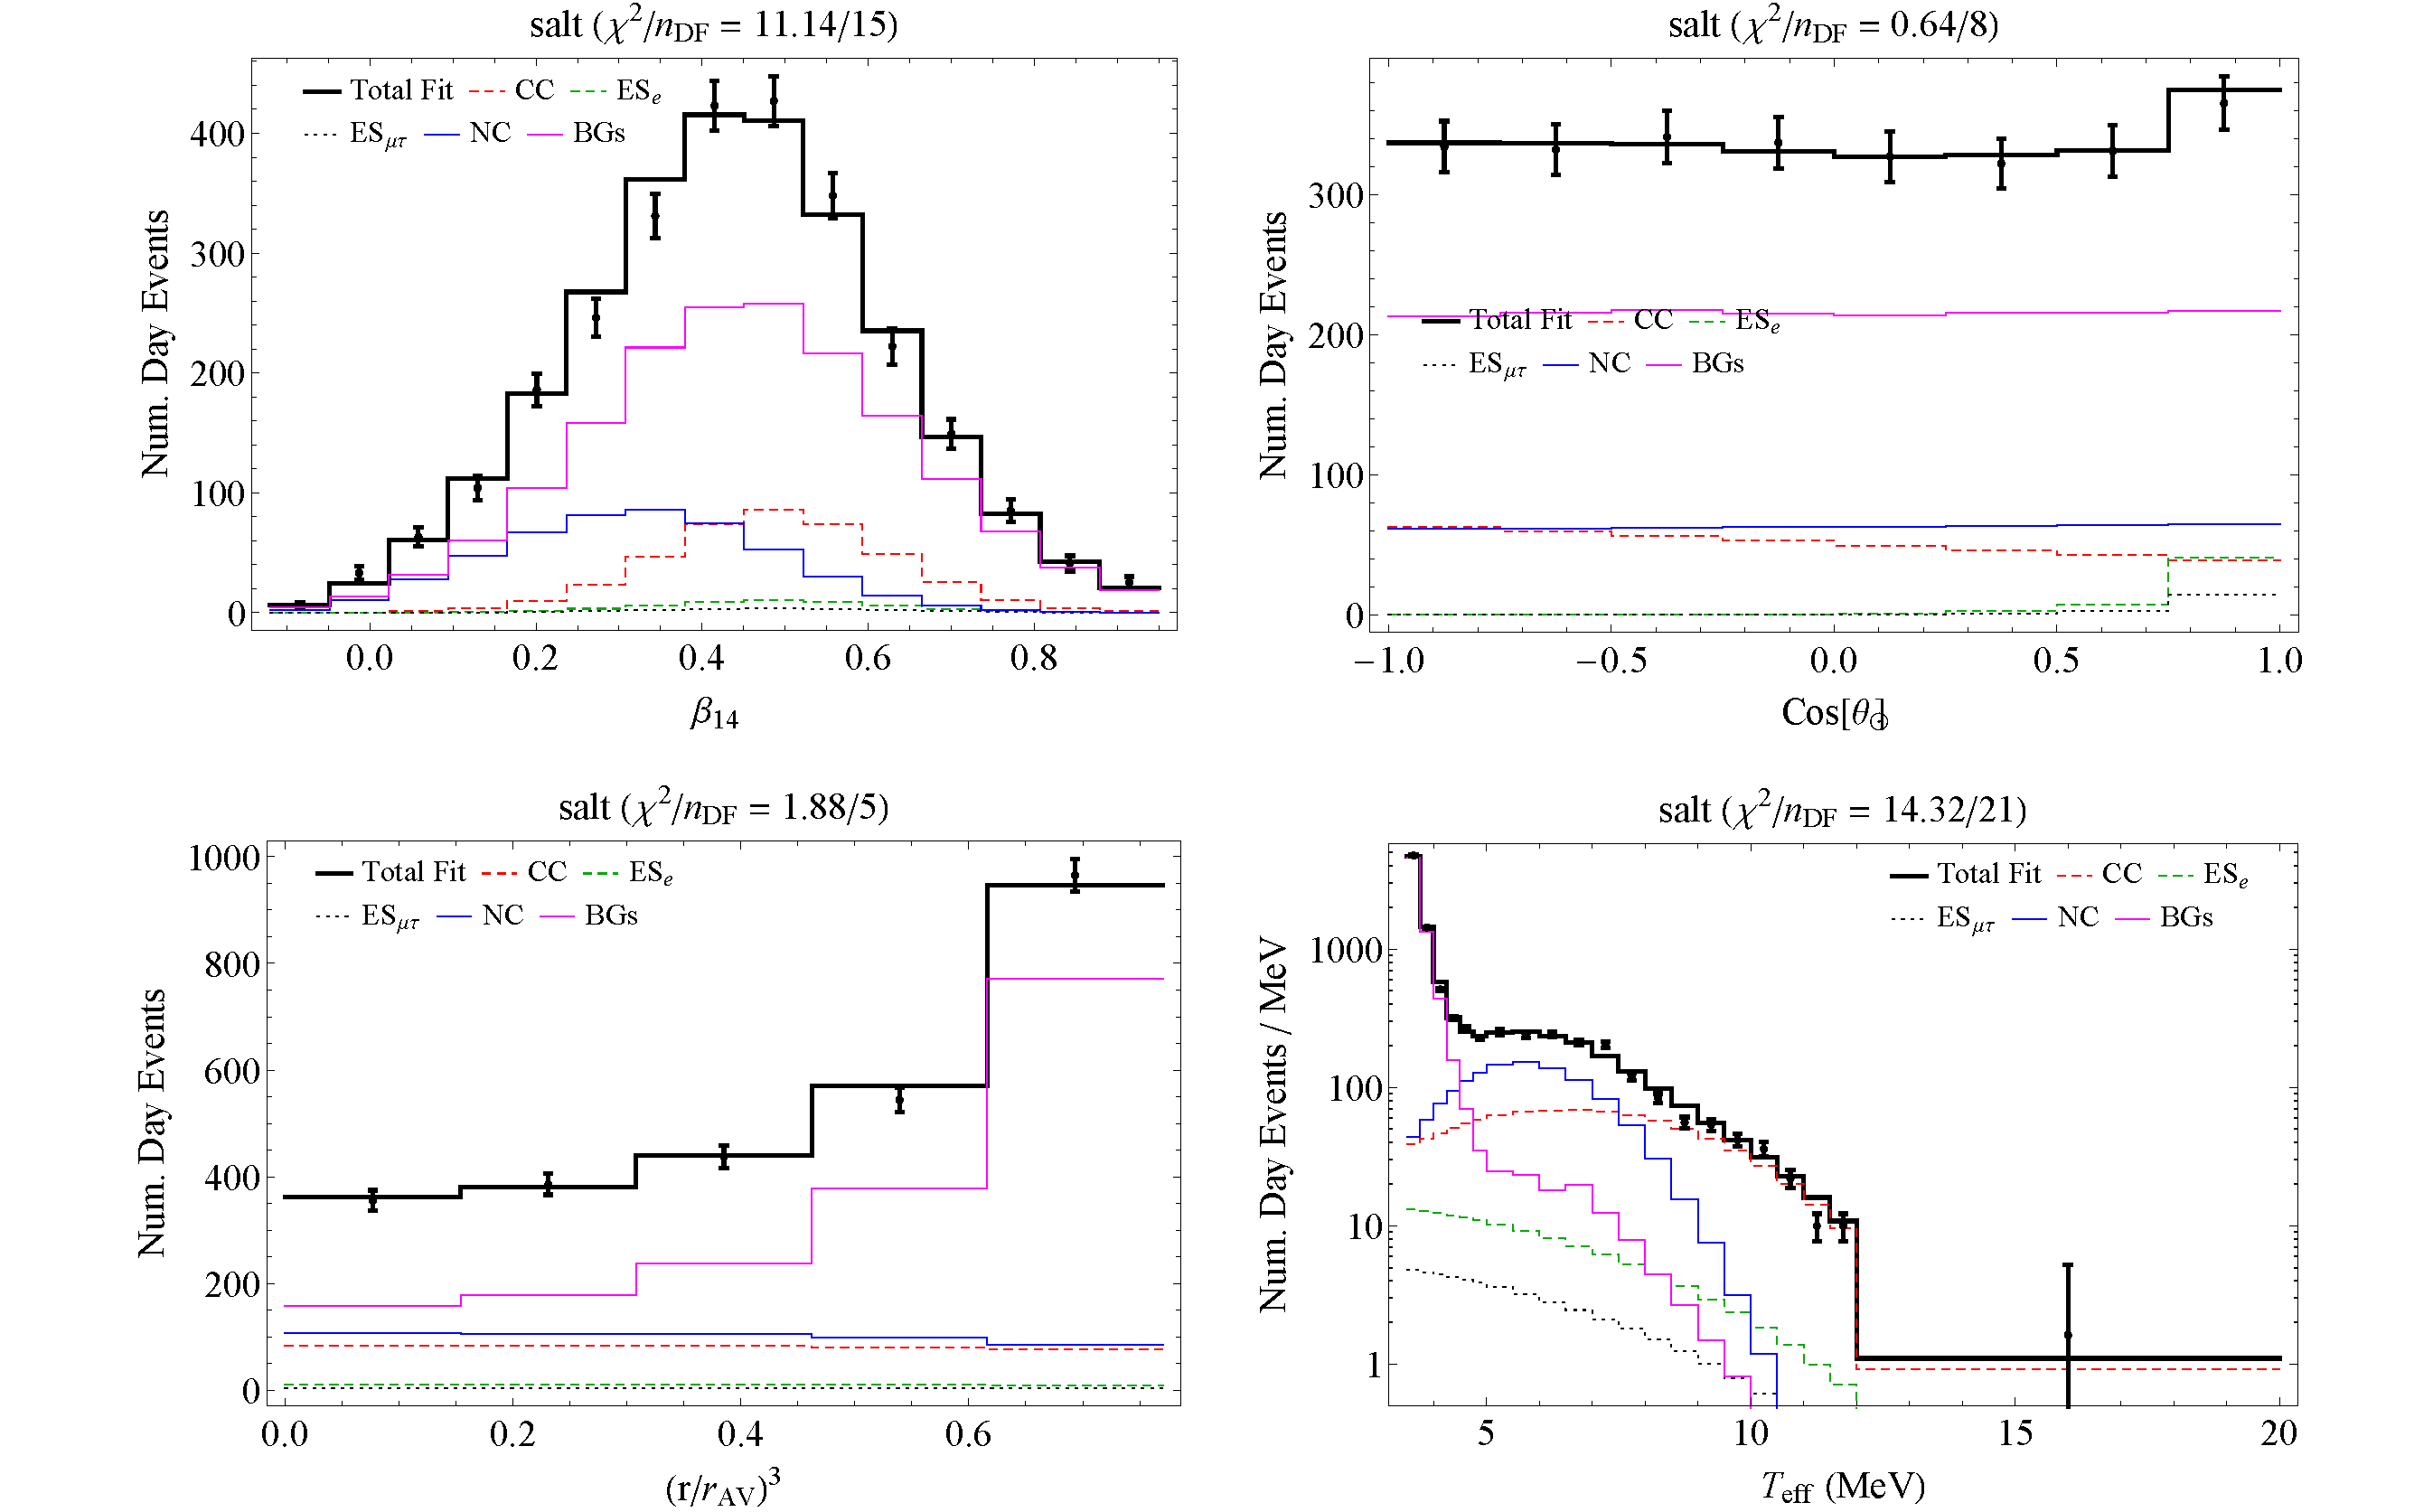
\includegraphics[width=0.95\columnwidth]{third_salt_day}
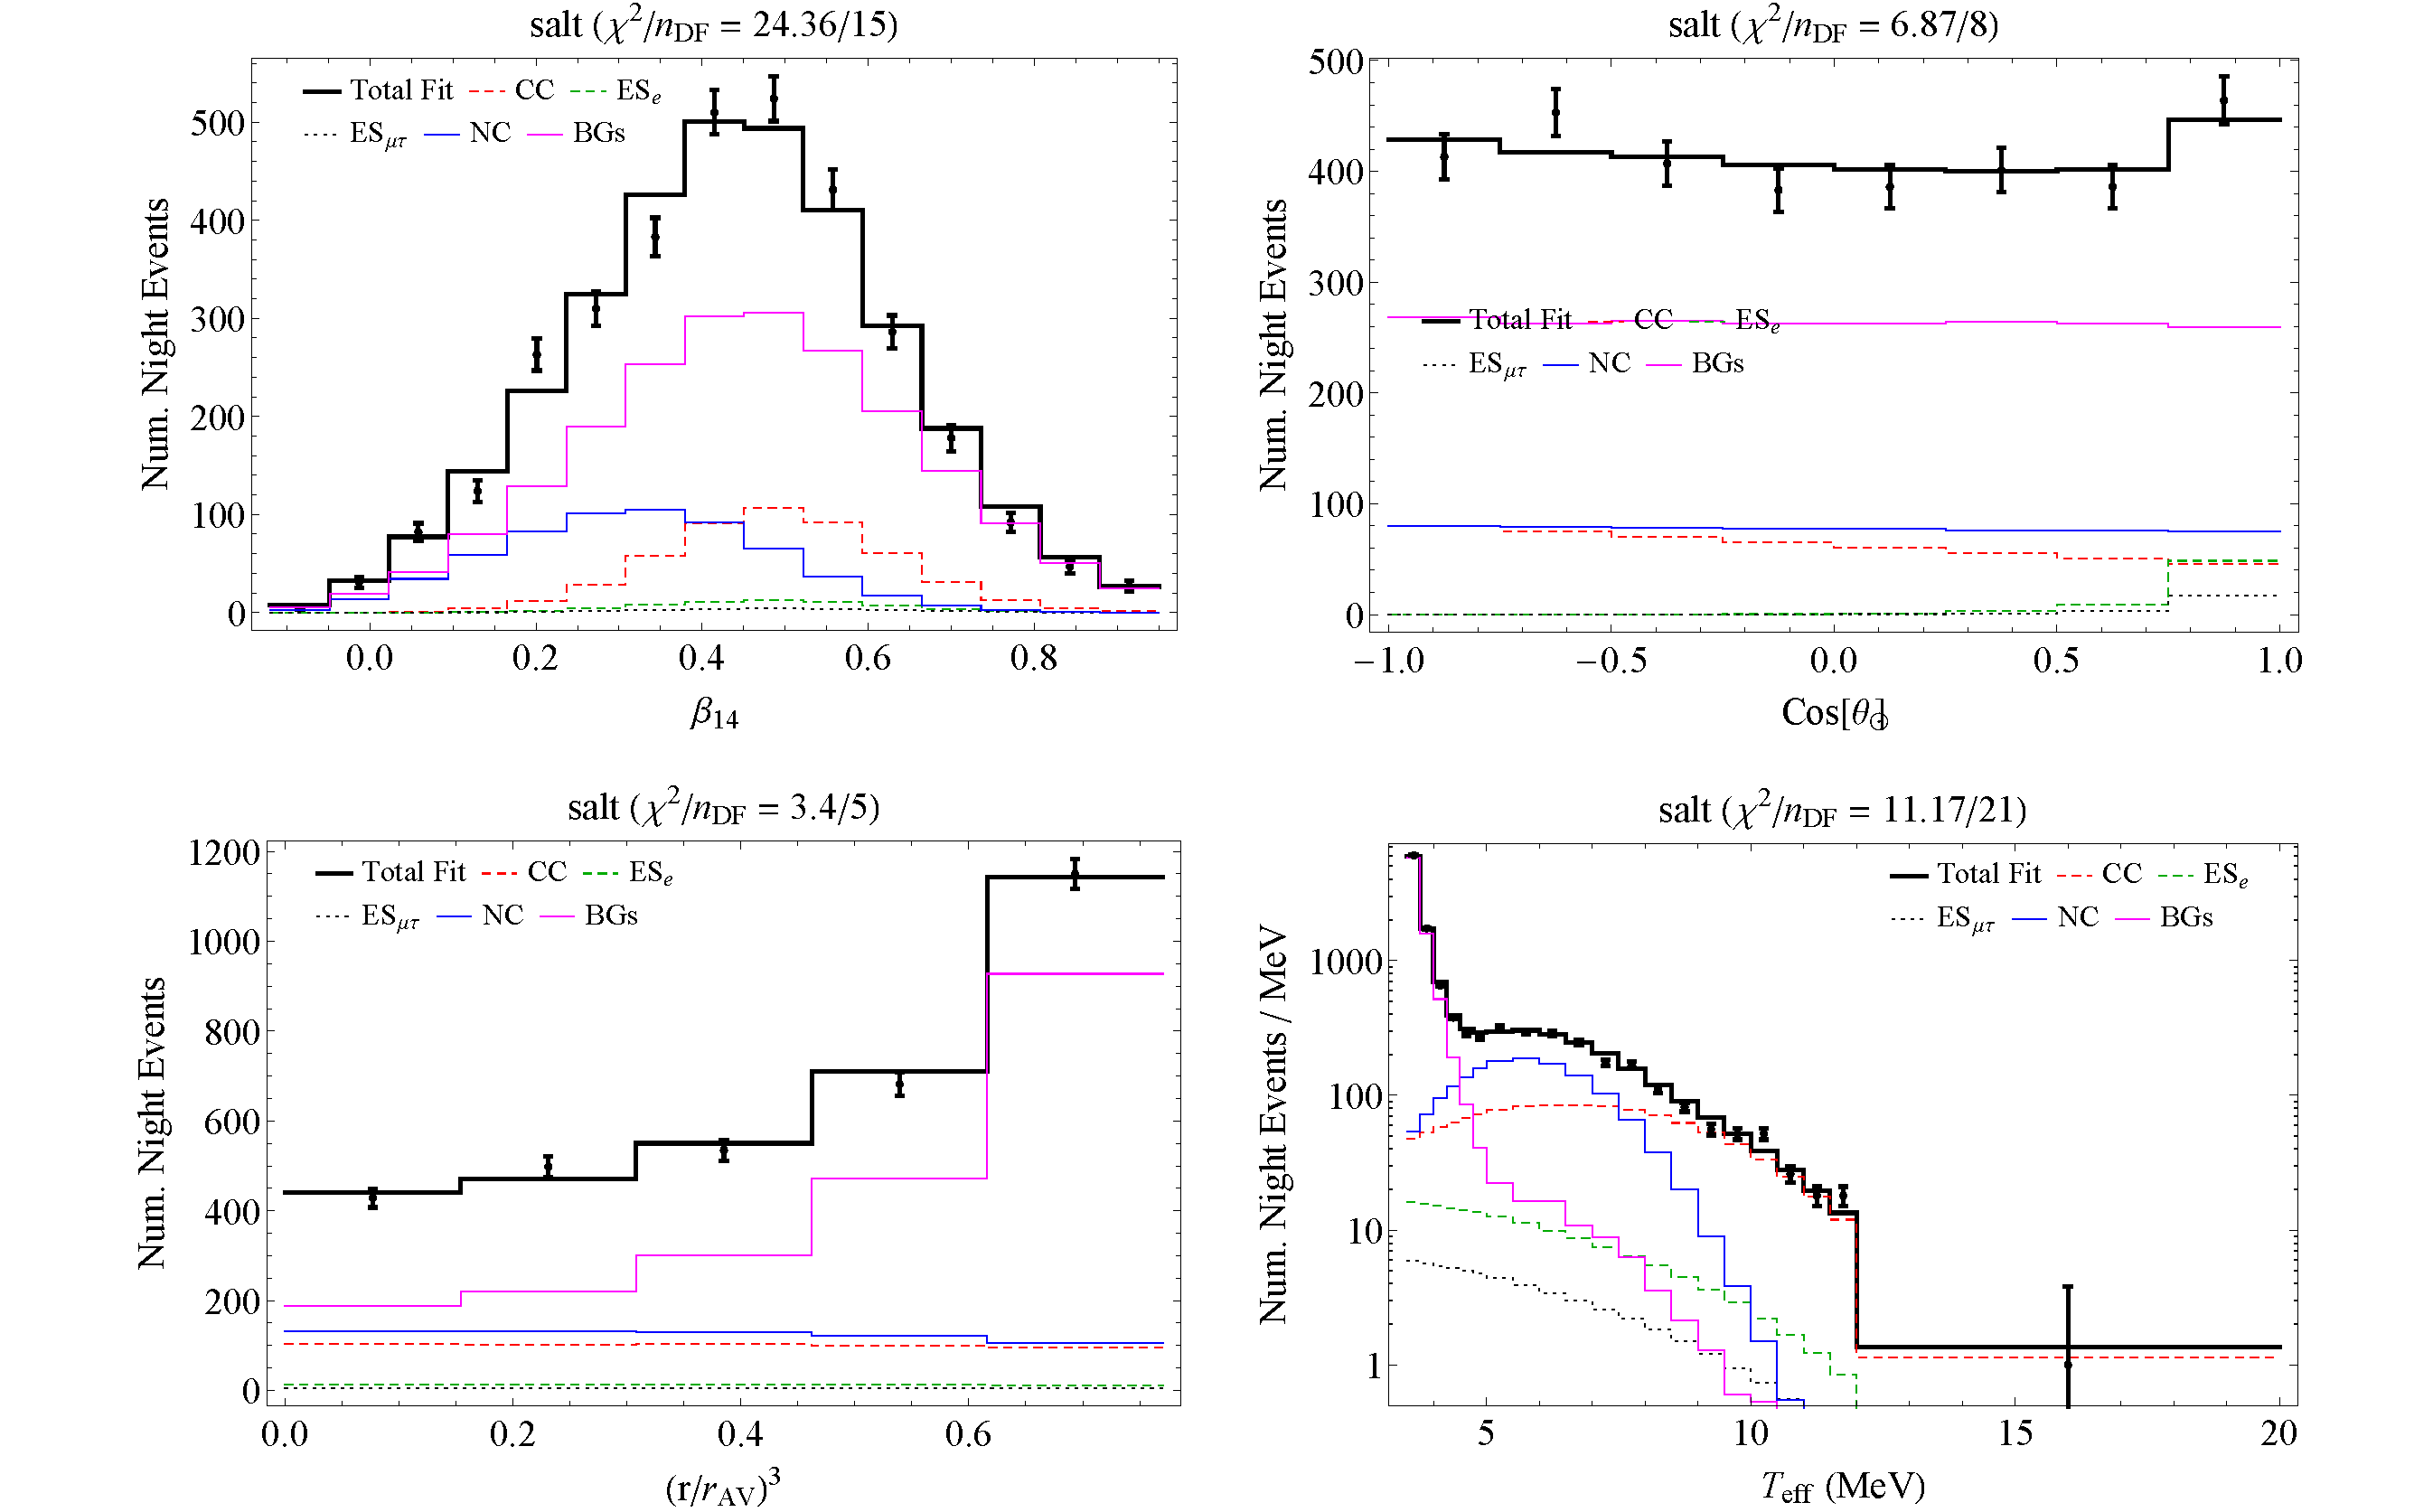
\includegraphics[width=0.95\columnwidth]{third_salt_night}
\caption{\label{fig:third_salt_obs}Observable distributions for Phase II for the 1/3 dataset fit.}
\end{figure}
\begin{figure}
\centering
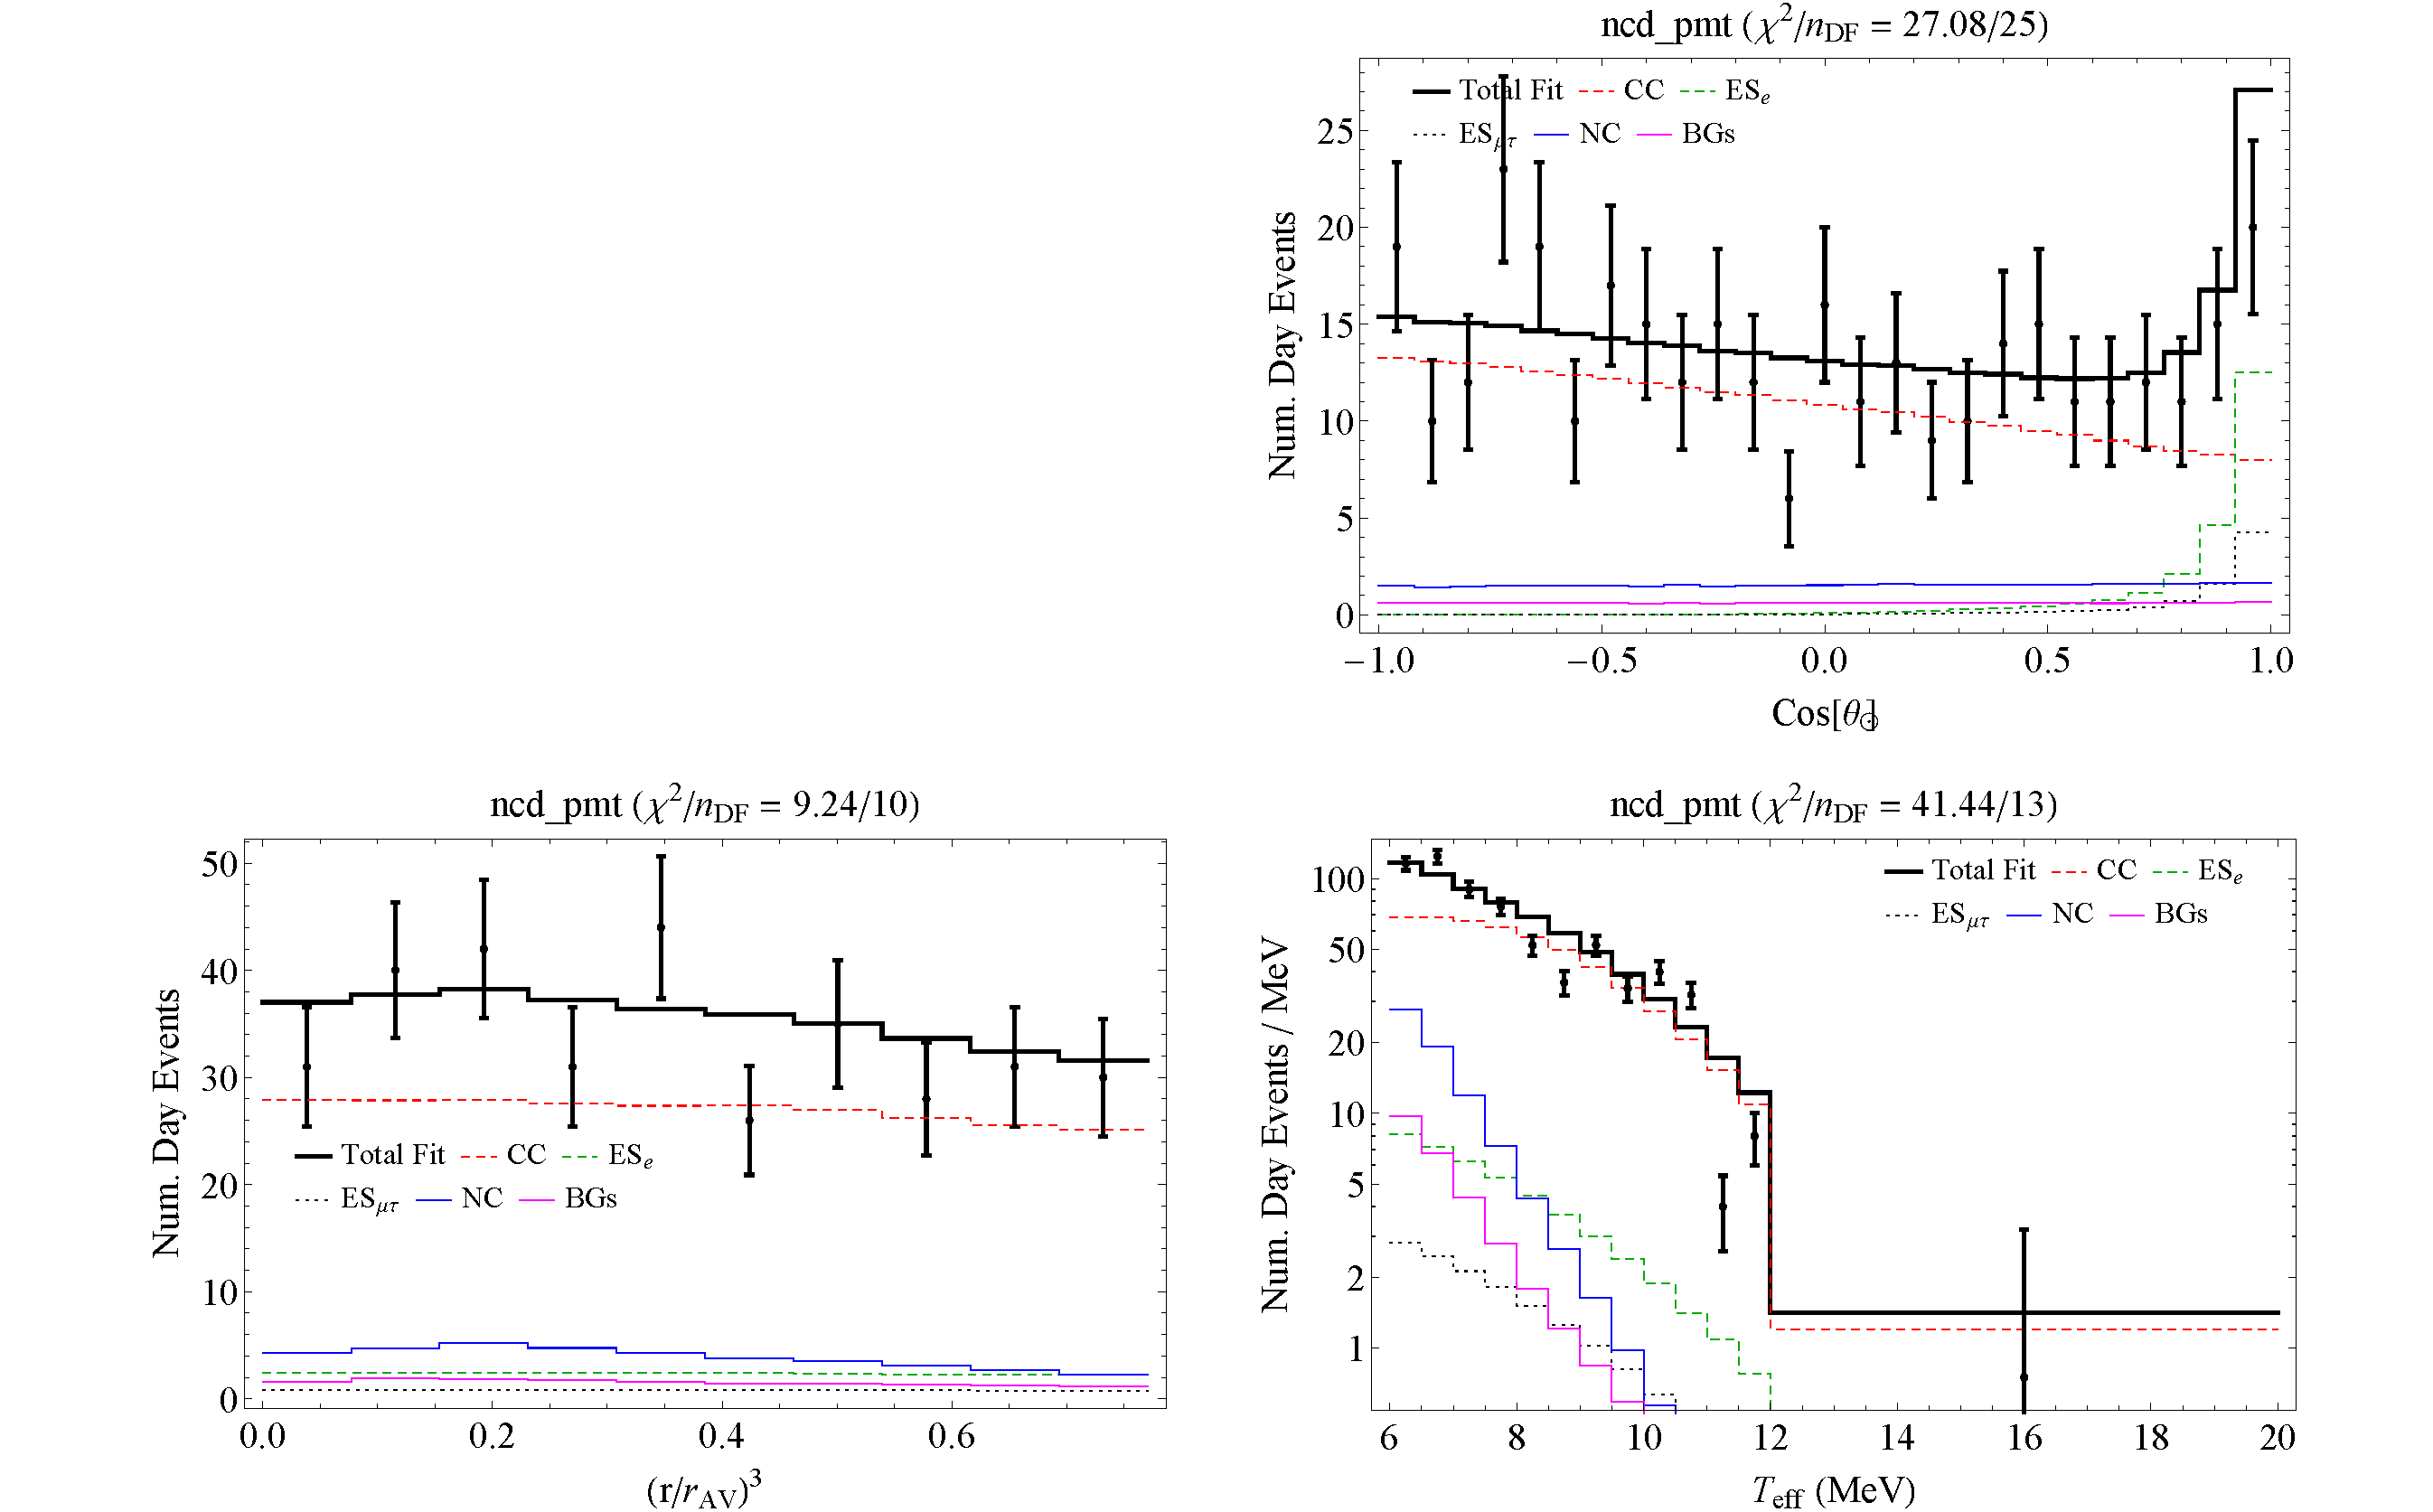
\includegraphics[width=0.95\columnwidth]{third_ncd_pmt_day}
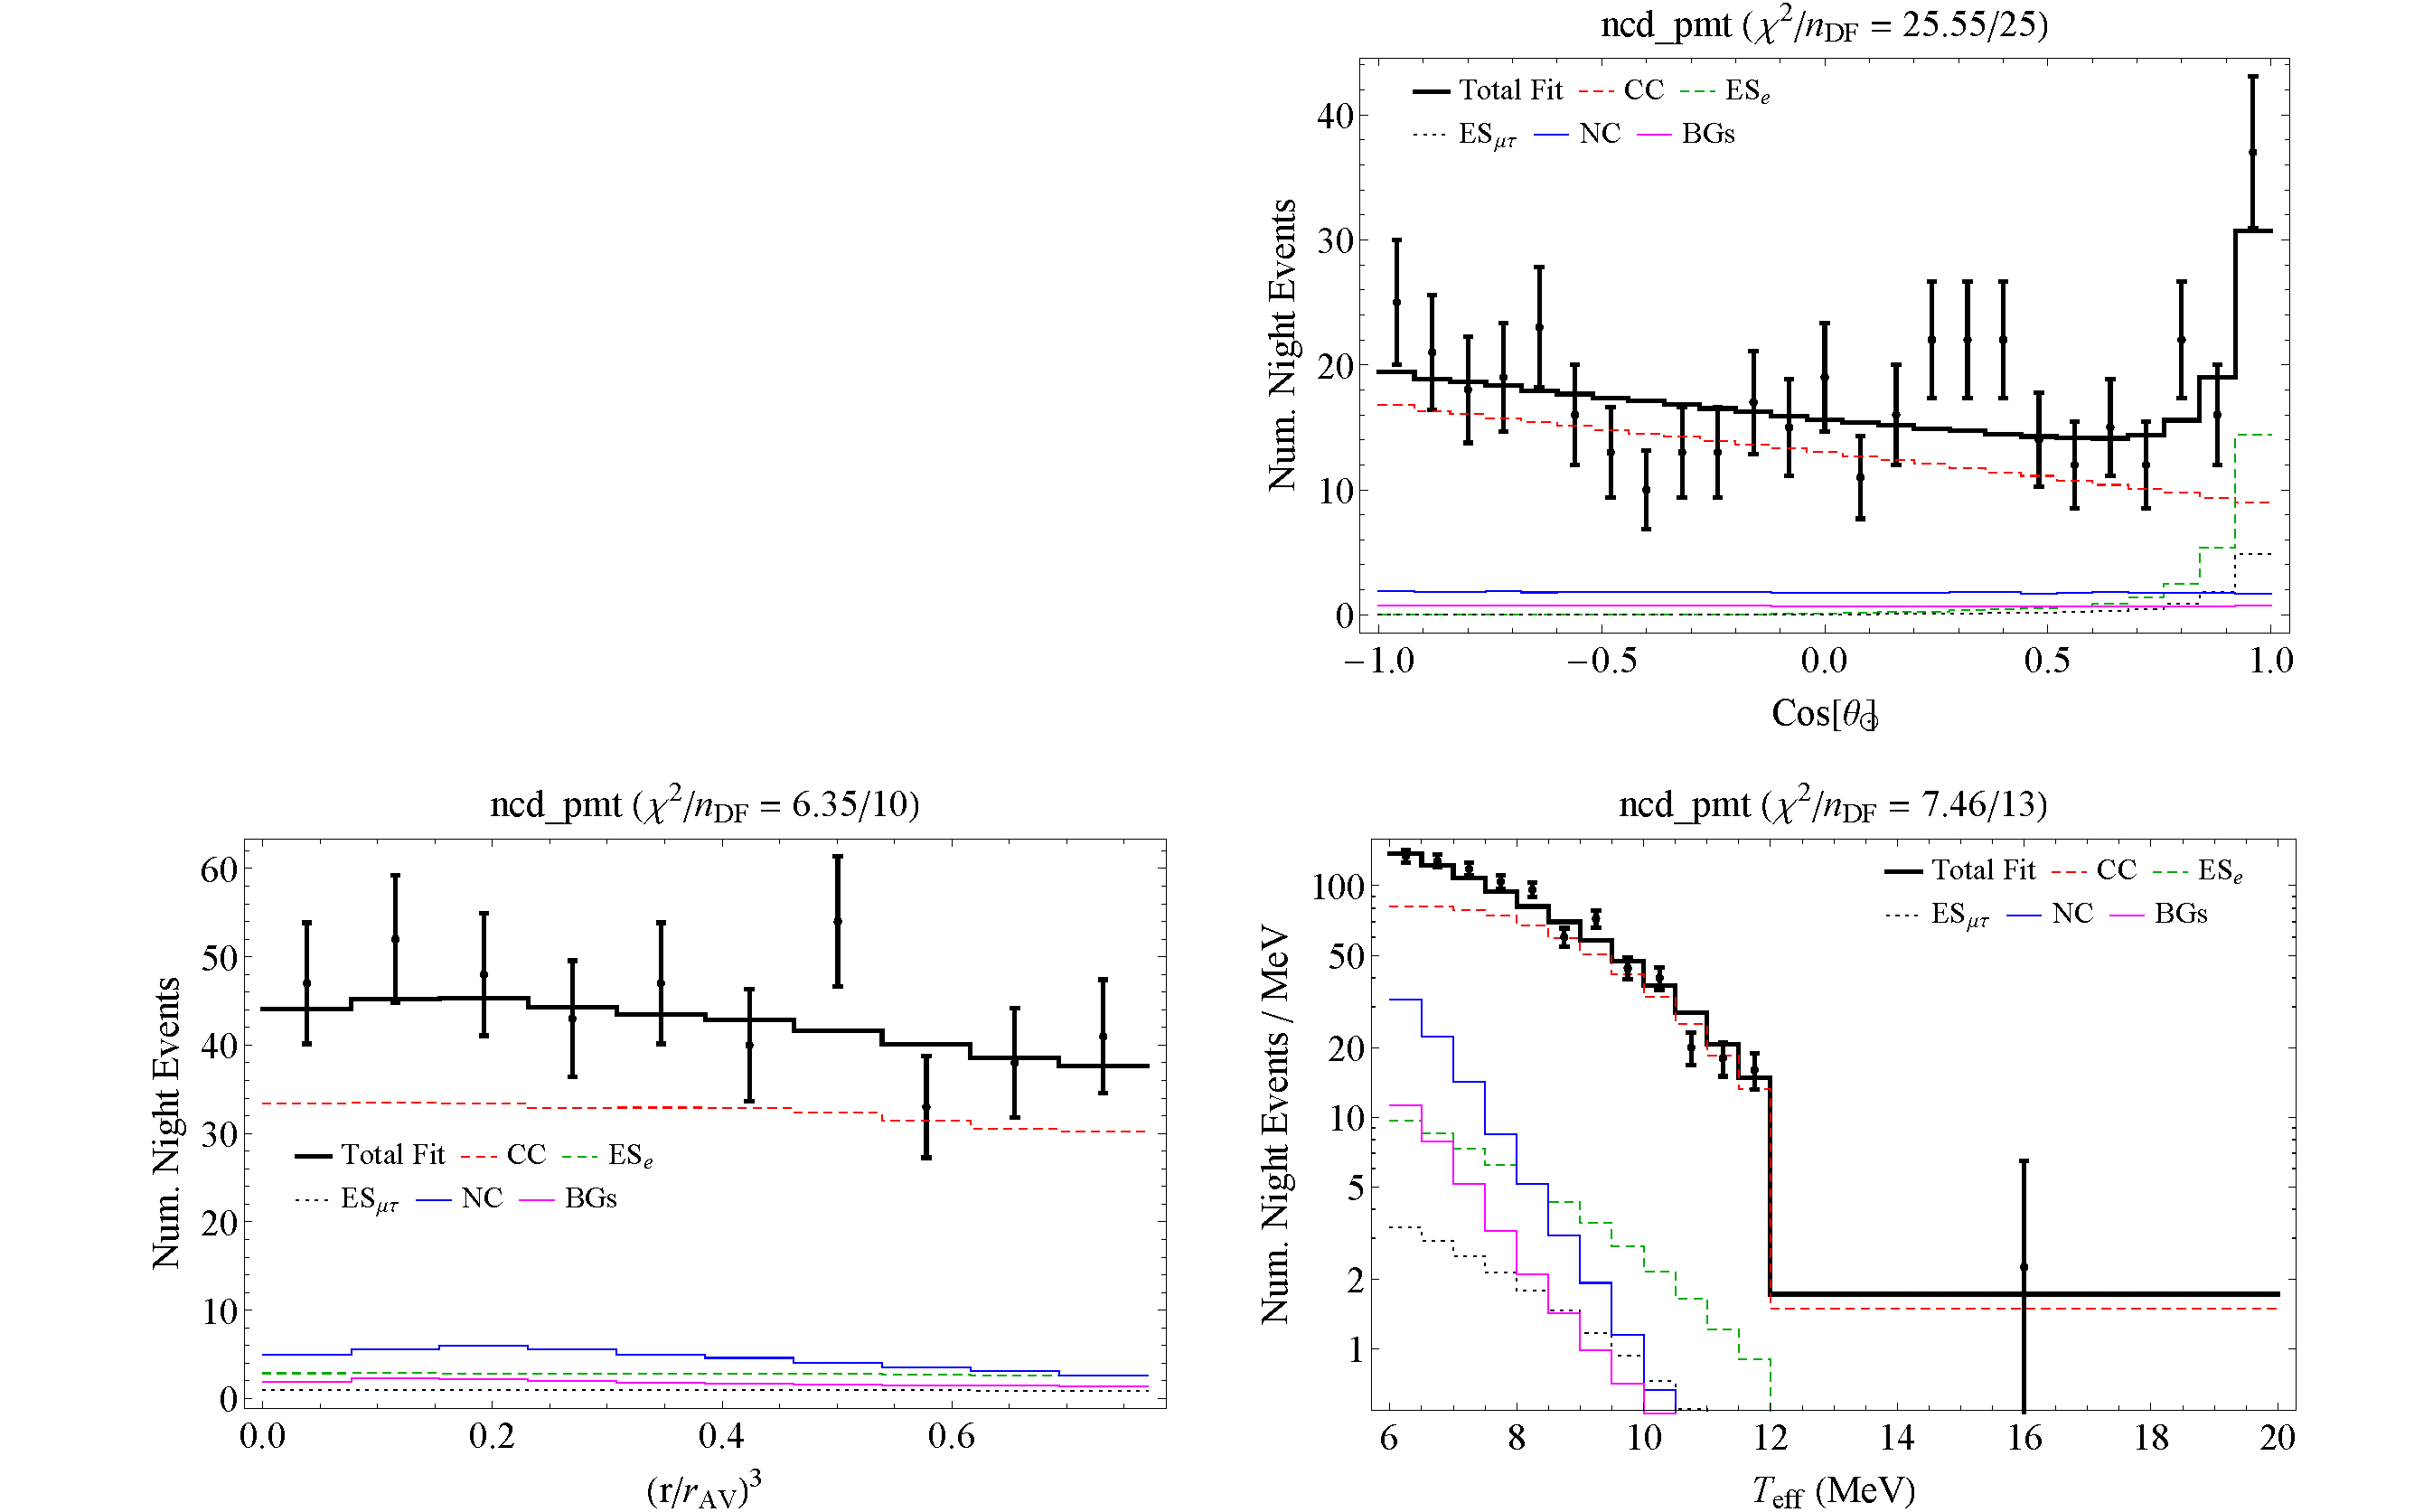
\includegraphics[width=0.95\columnwidth]{third_ncd_pmt_night}
\caption{\label{fig:third_ncd_pmt_obs}Observable distributions for Phase IIIb for the 1/3 dataset fit. Note that $\beta_{14}$ was not used in analyses for Phase IIIb.}
\end{figure}

\clearpage

\subsection{\texorpdfstring{$k_2$}{k2} Fixed to Infinity}

Shown in \Cref{fig:third_inf_d2o_obs,fig:third_inf_salt_obs,fig:third_inf_ncd_pmt_obs} are the observable distributions for a 3 phase fit to the 1/3 dataset with no decay ($k_2$ fixed at infinity). These plots are provided primarily as a cross check.

\begin{figure}
\centering
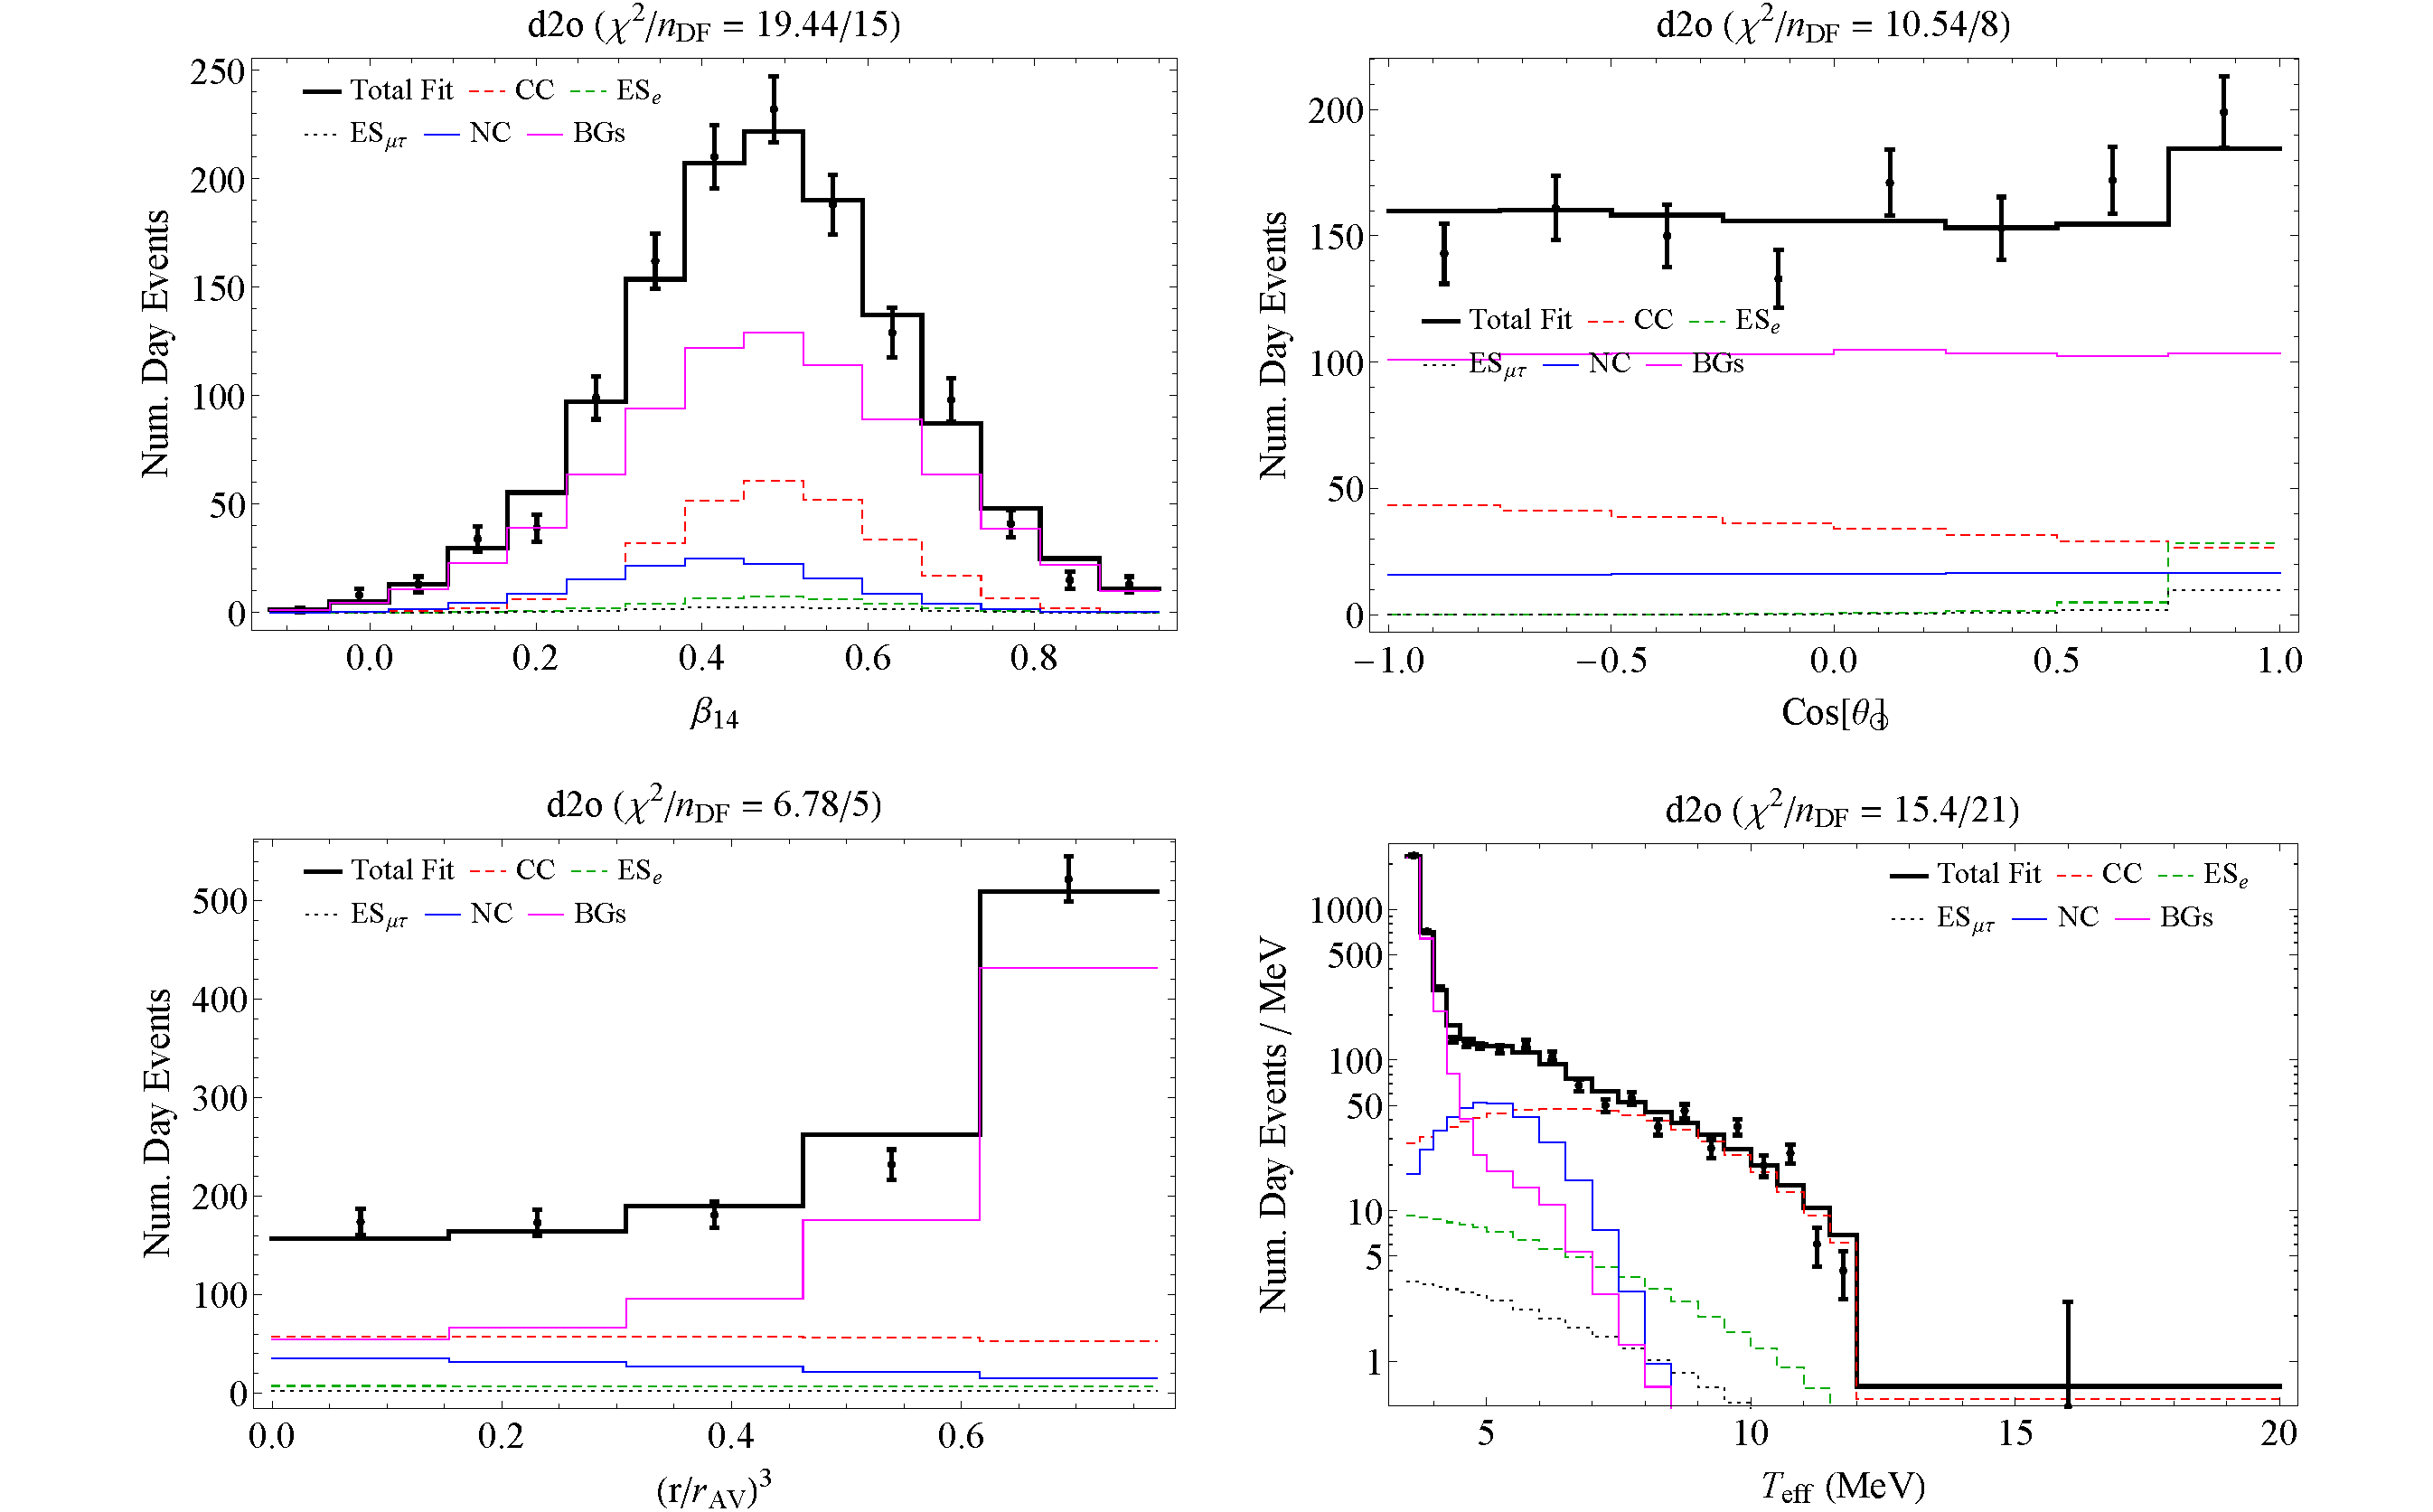
\includegraphics[width=0.95\columnwidth]{third_inf_d2o_day}
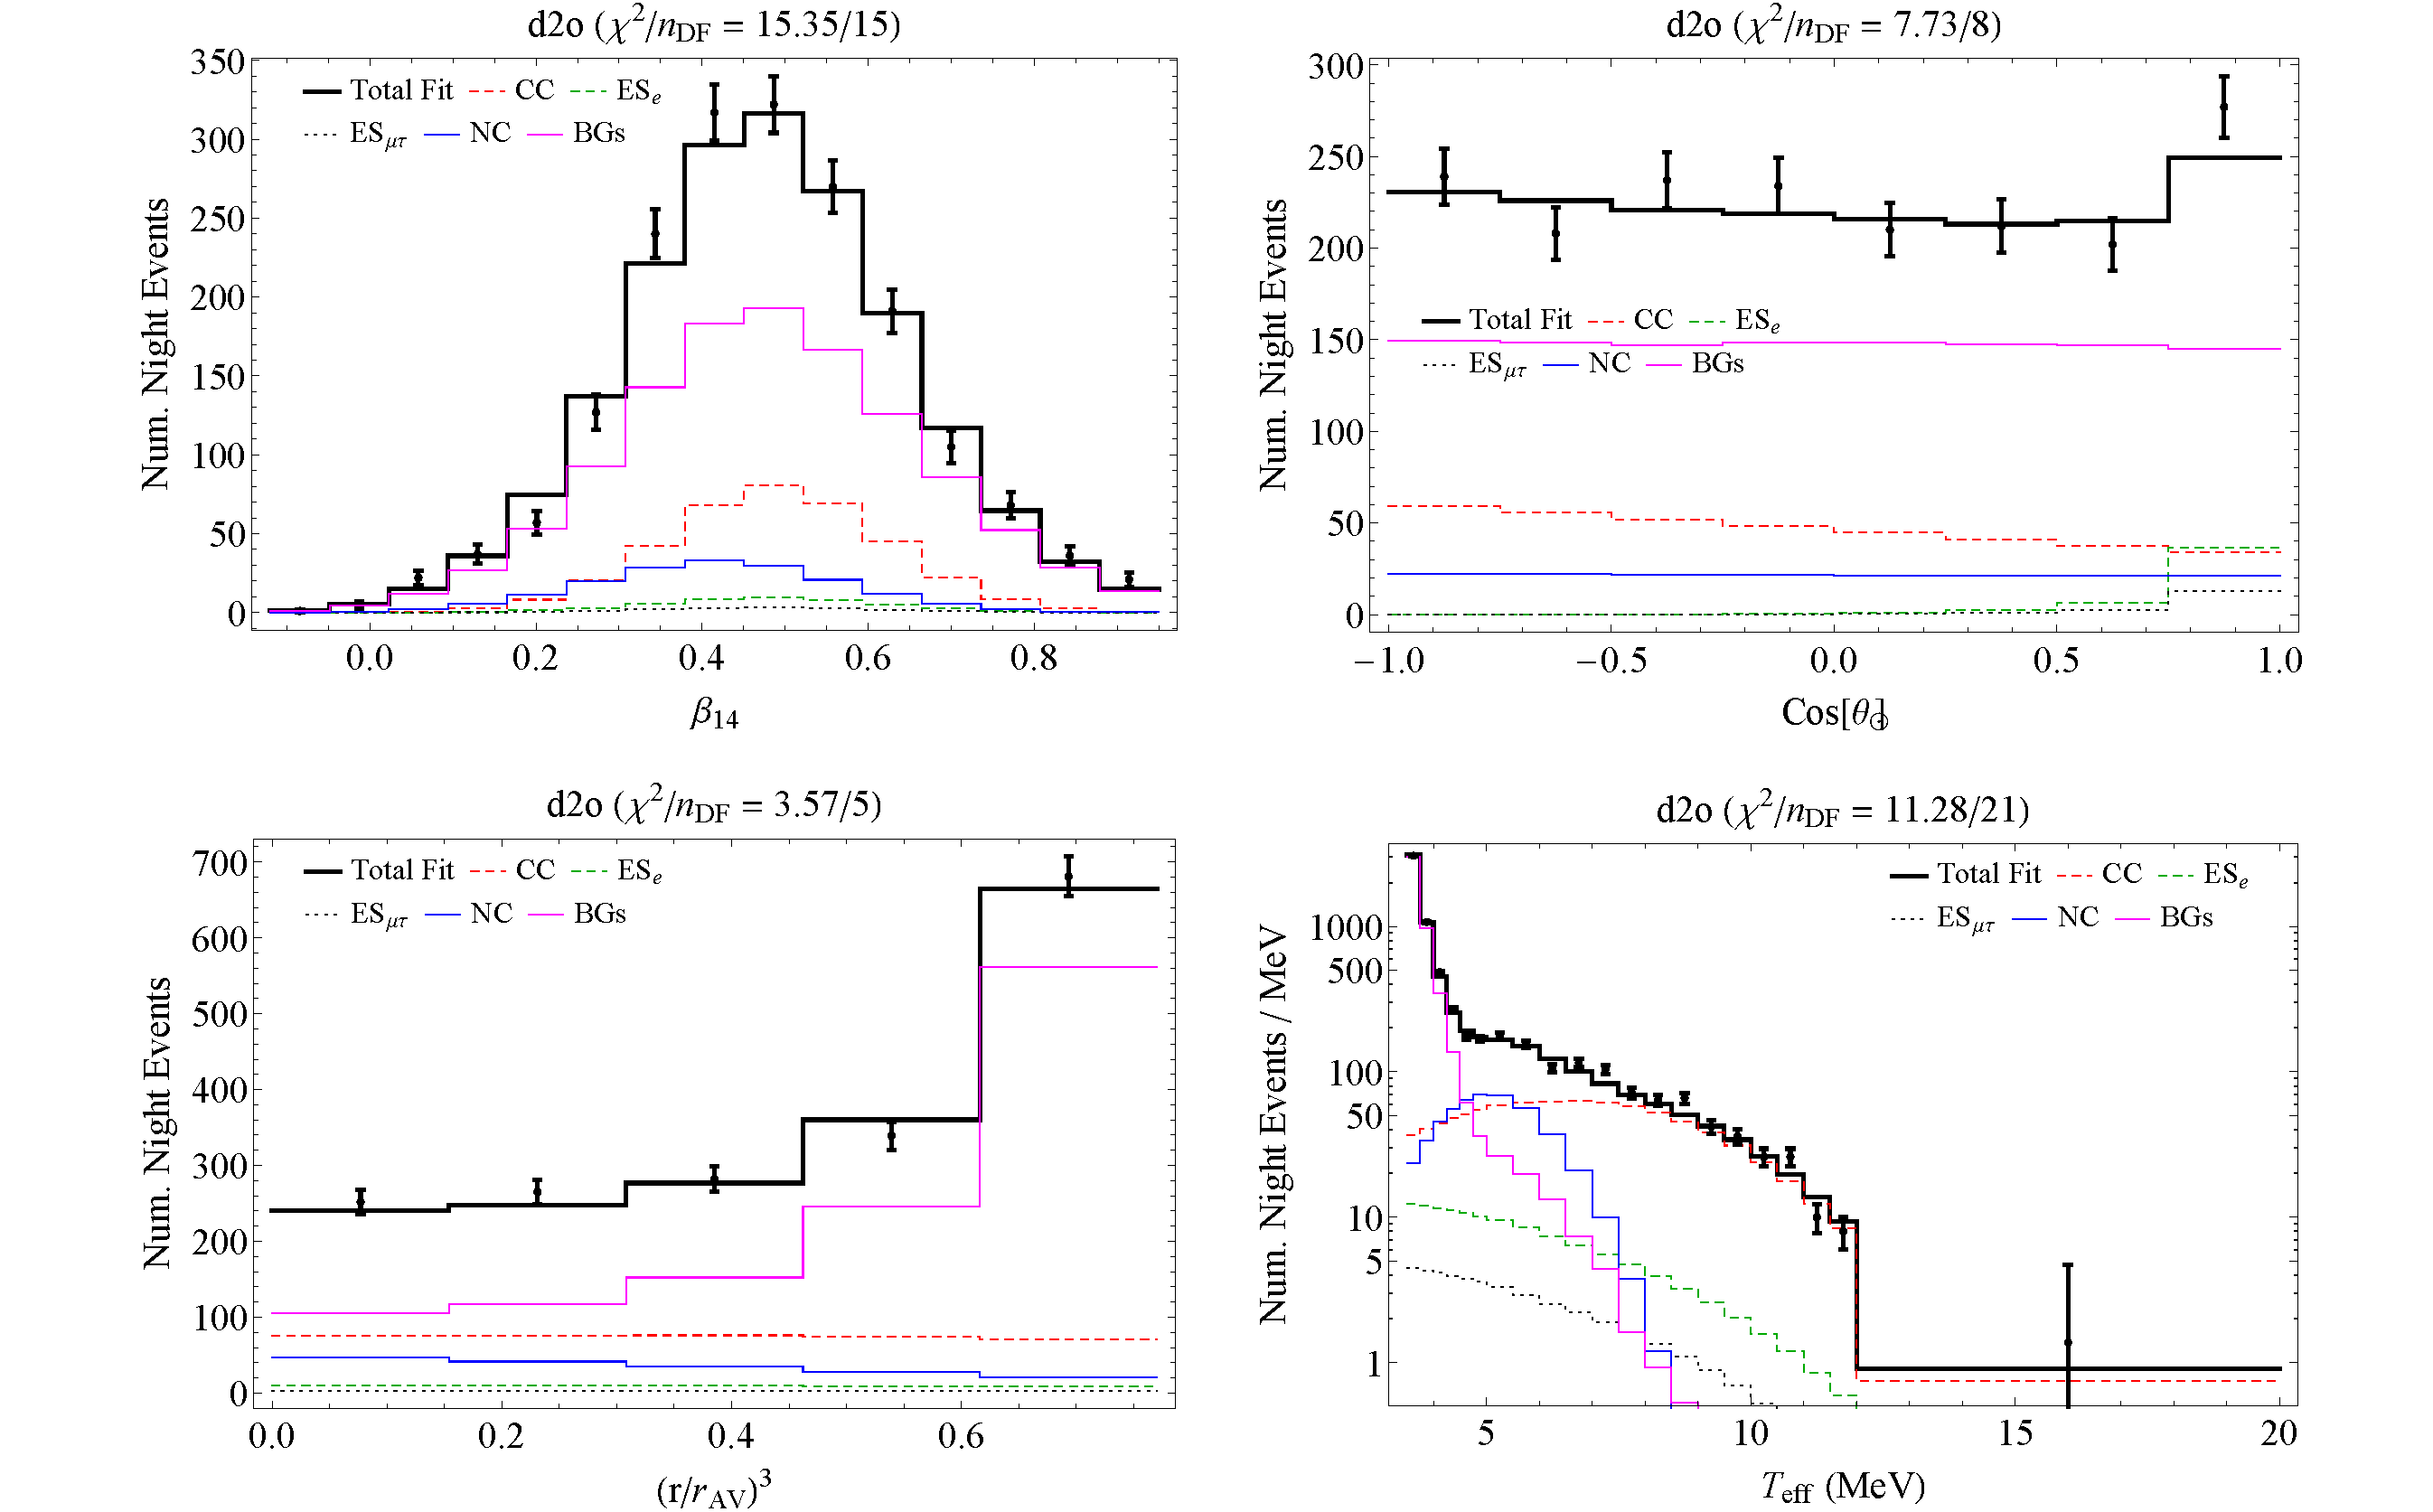
\includegraphics[width=0.95\columnwidth]{third_inf_d2o_night}
\caption{\label{fig:third_inf_d2o_obs}Observable distributions for Phase I for the 1/3 dataset fit with $k_2$ fixed to infinity.}
\end{figure}
\begin{figure}
\centering
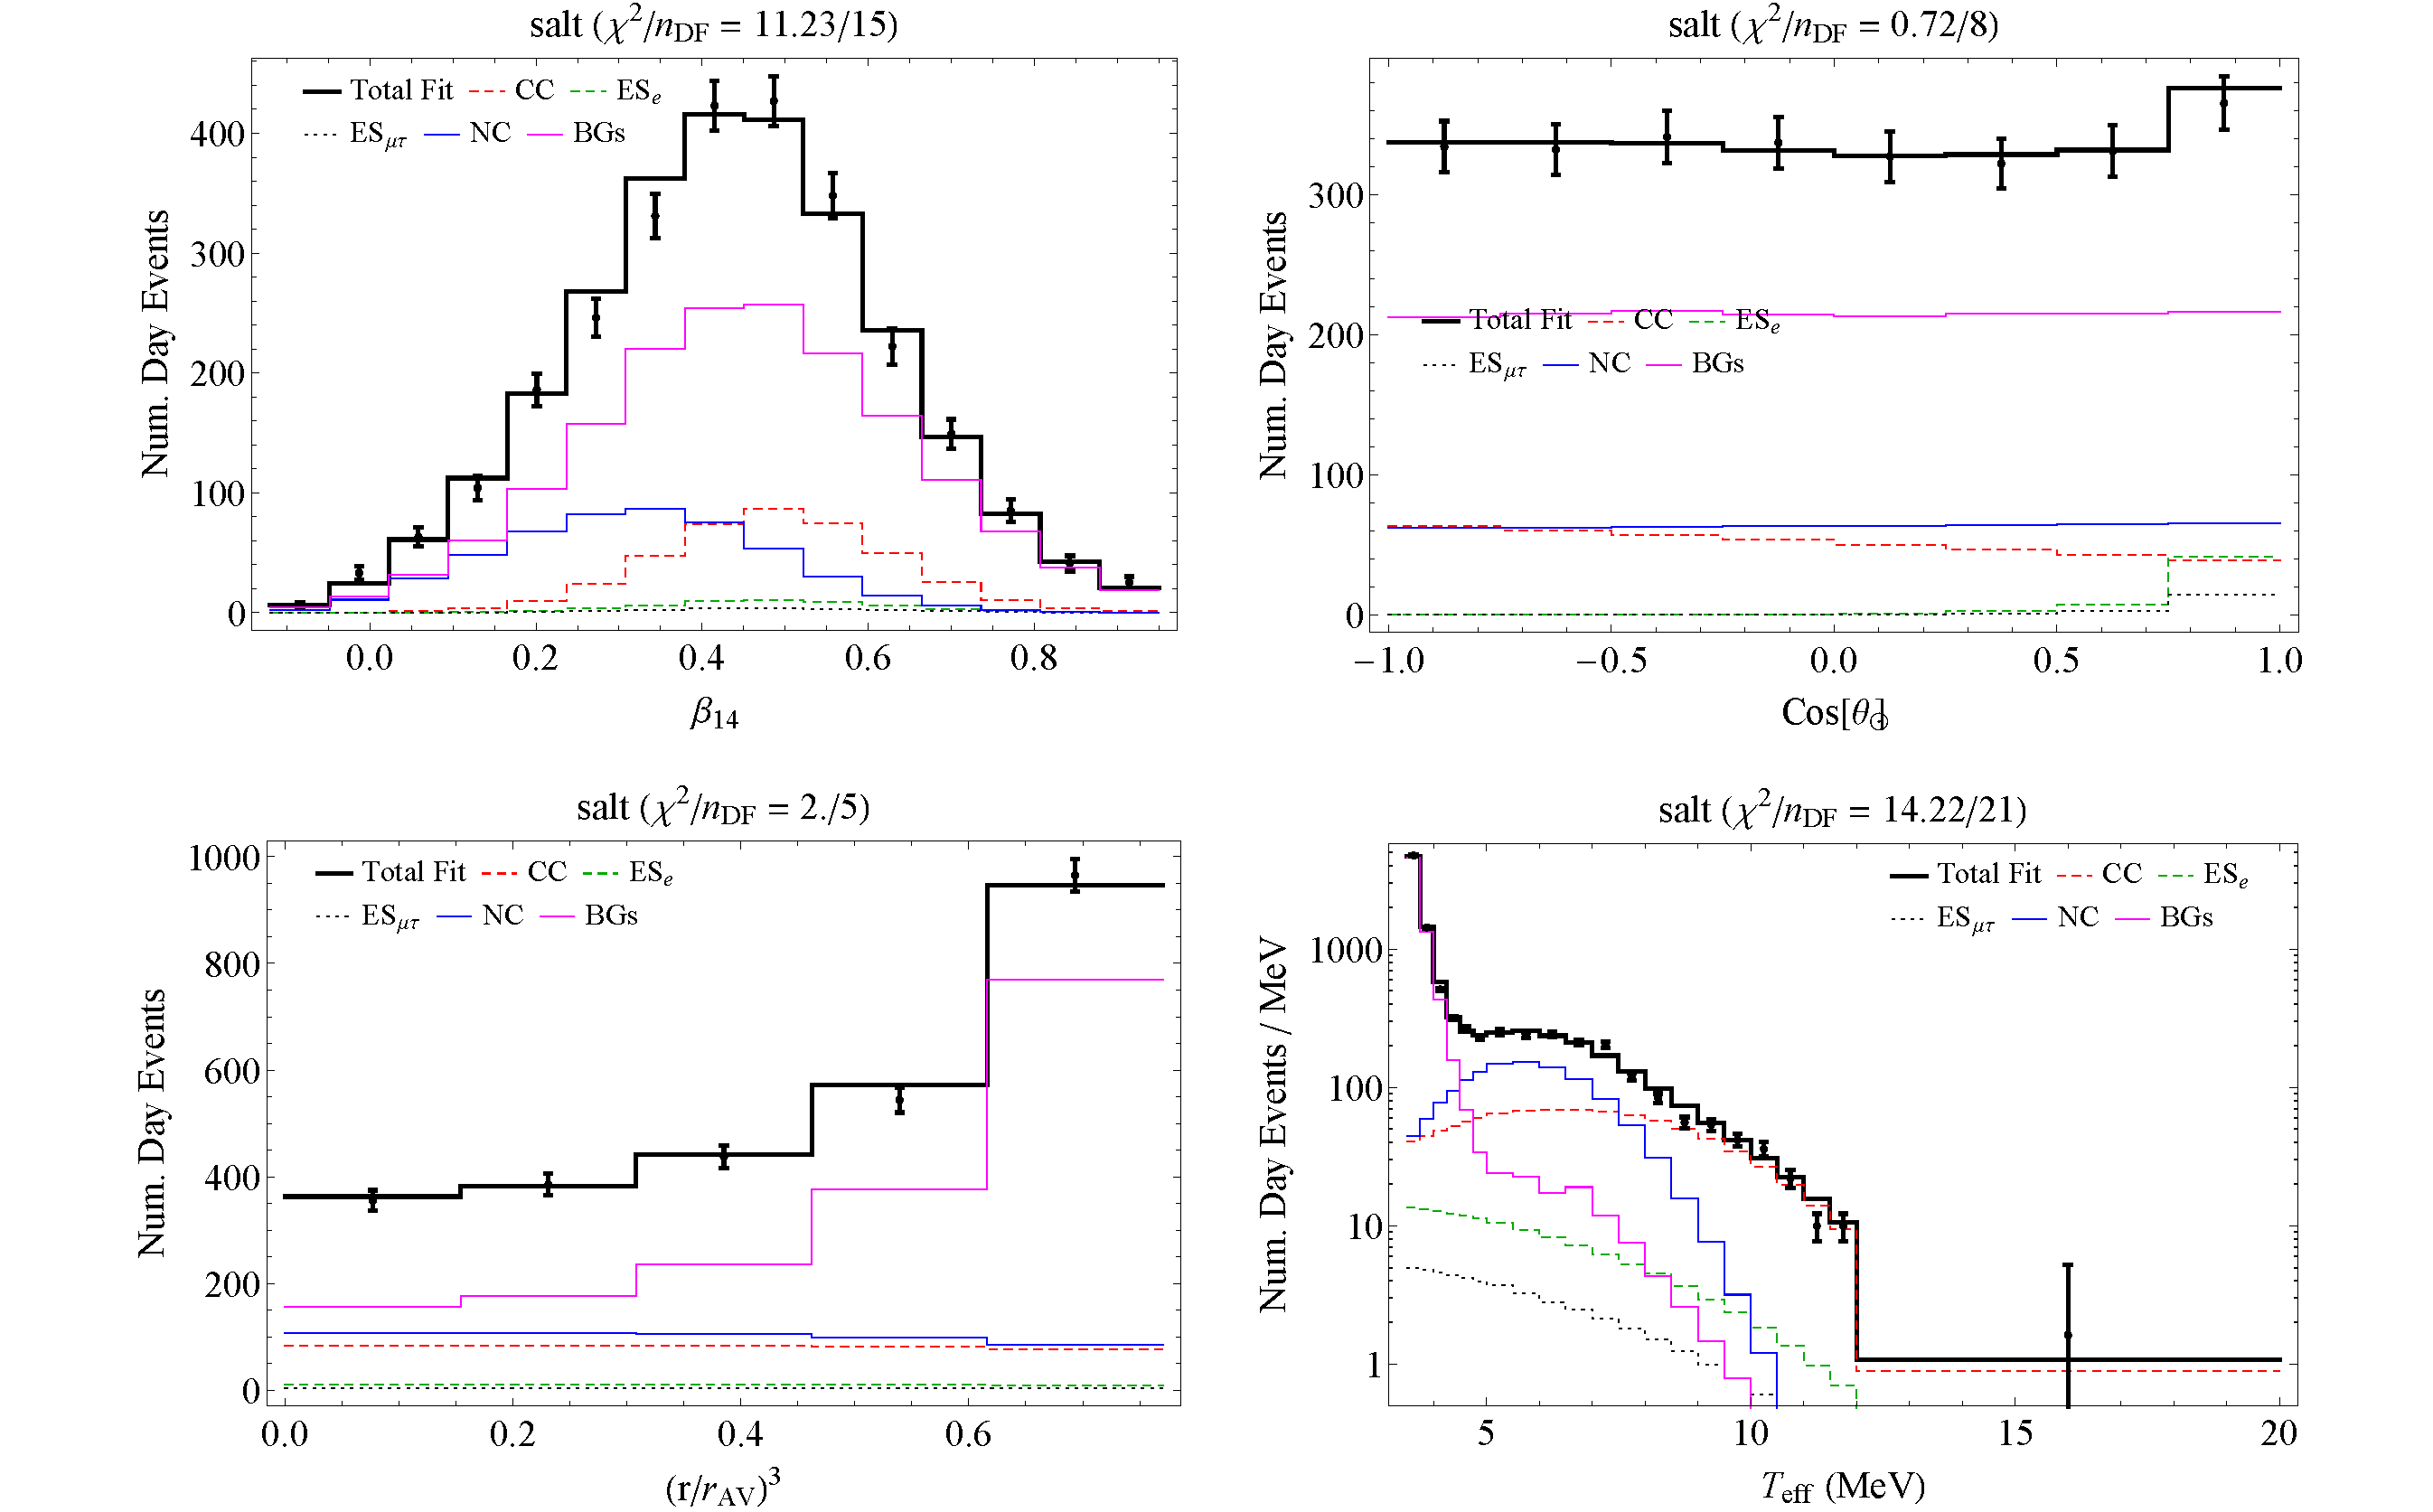
\includegraphics[width=0.95\columnwidth]{third_inf_salt_day}
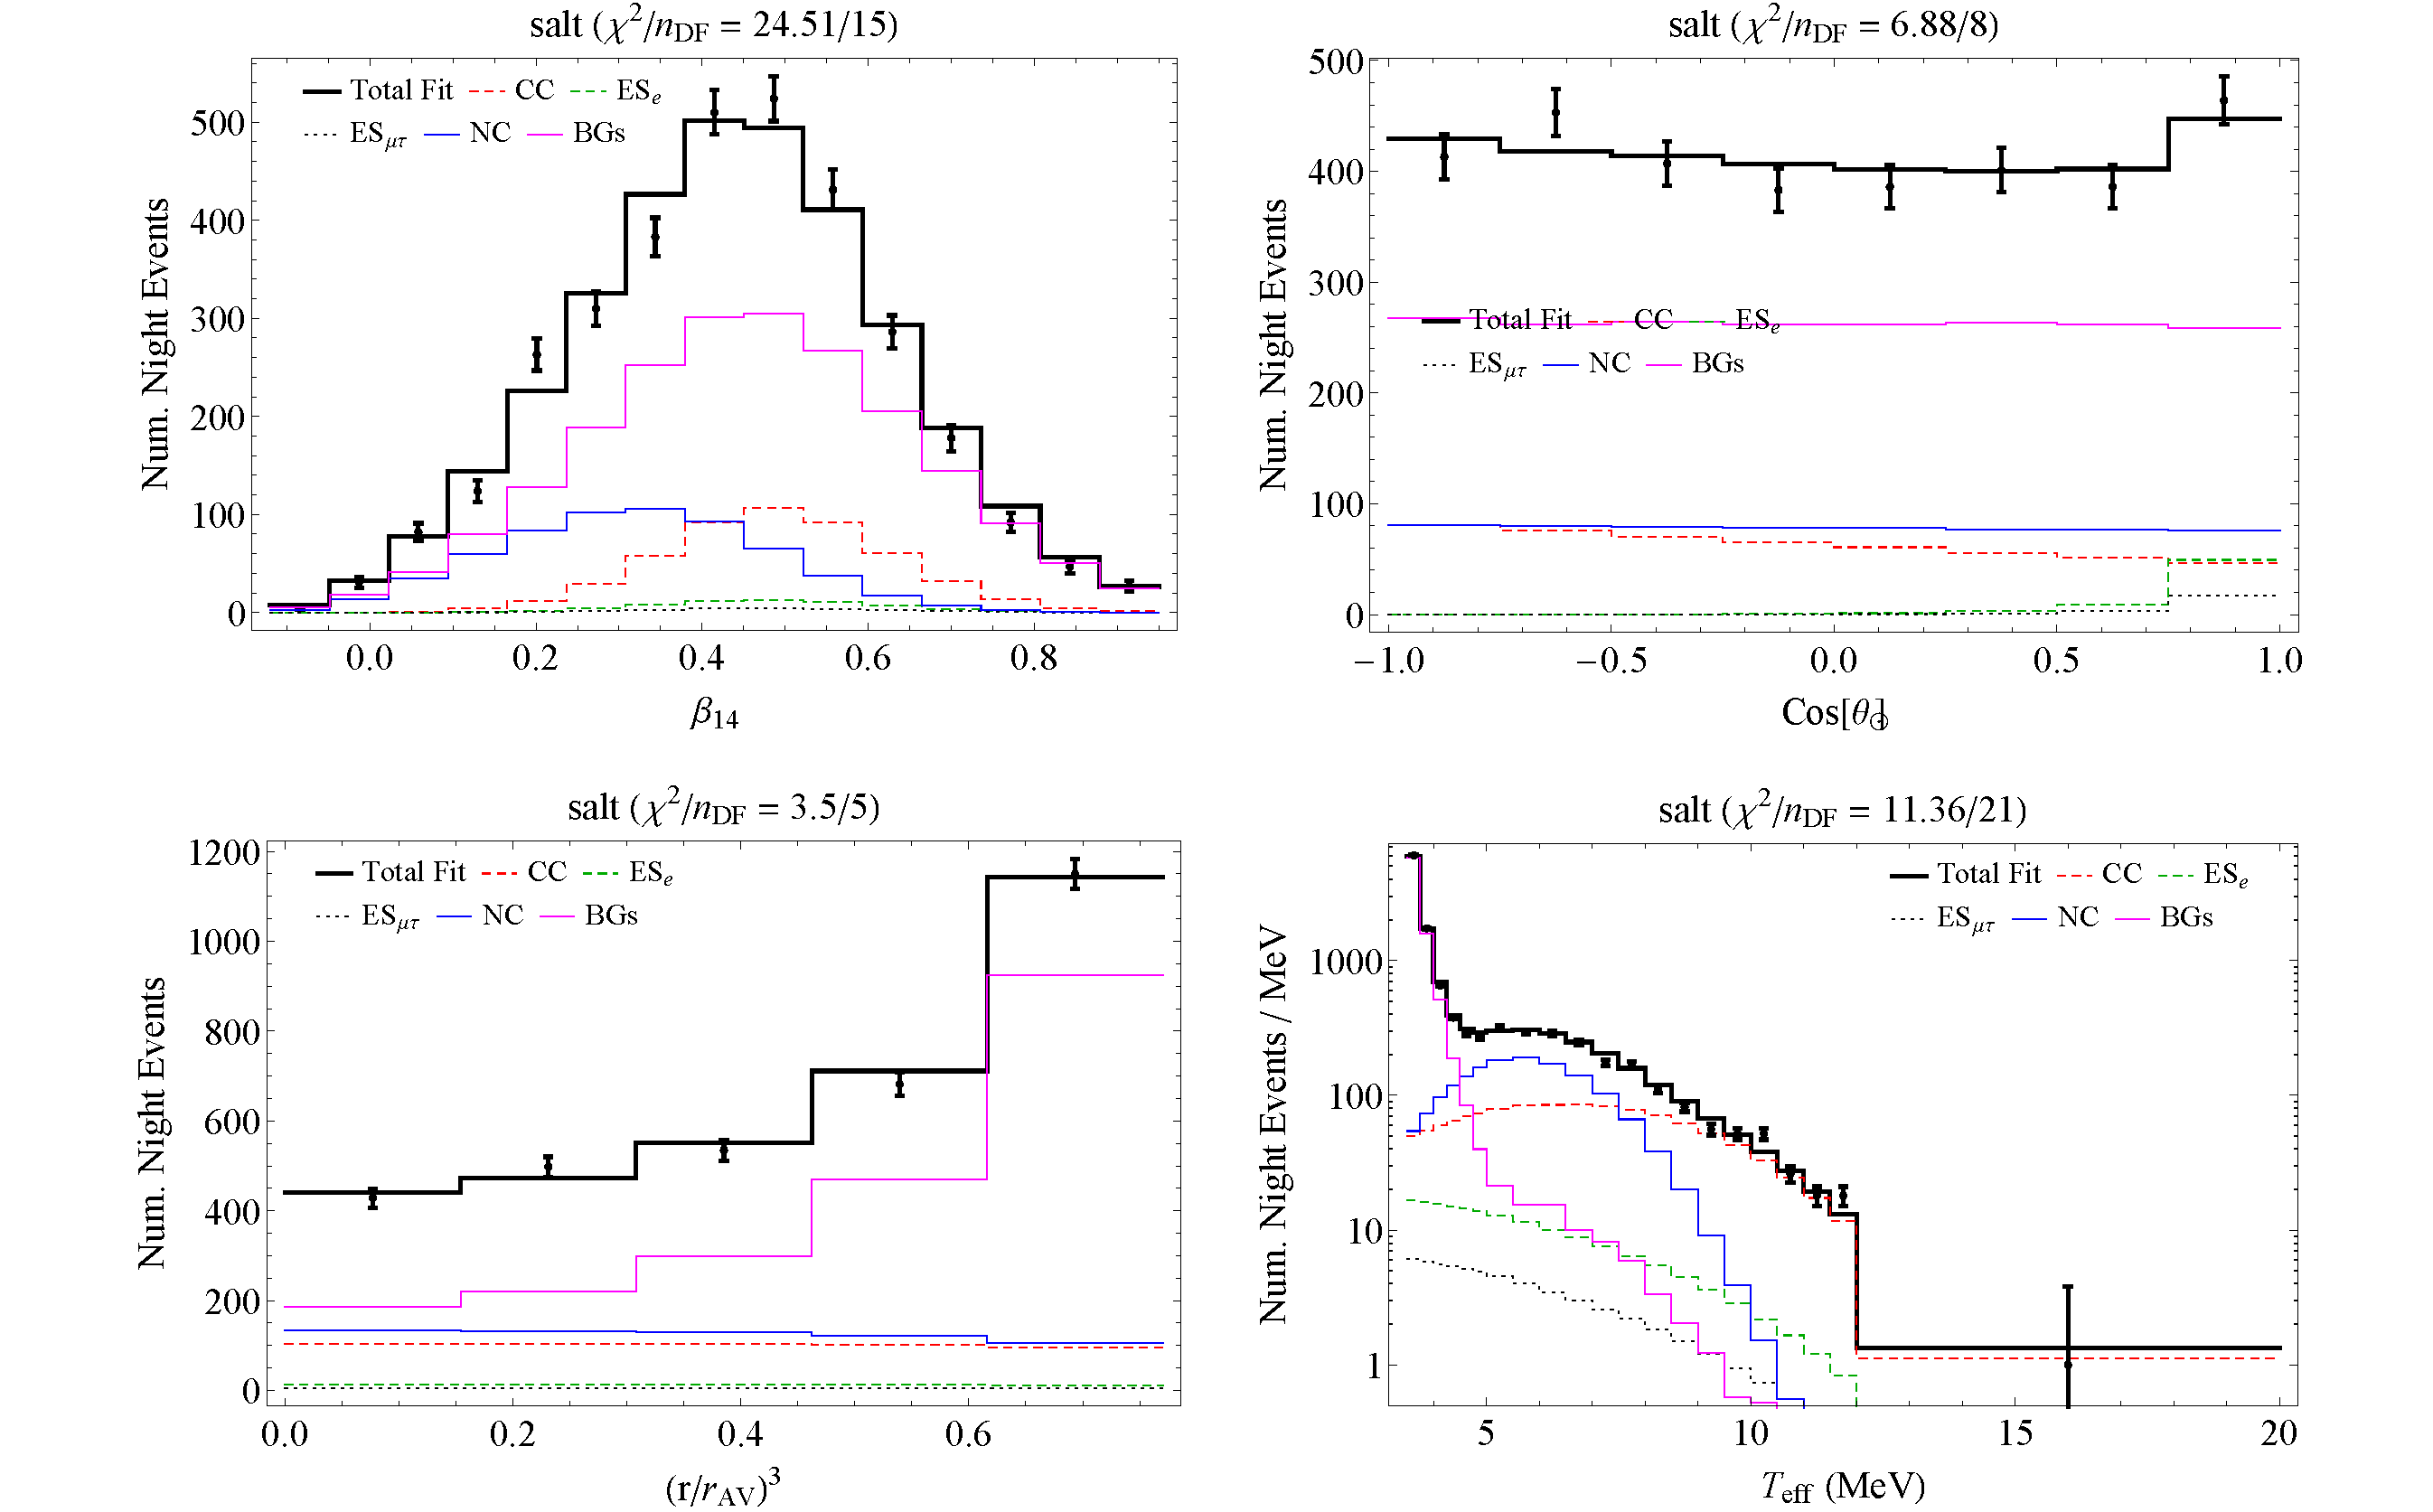
\includegraphics[width=0.95\columnwidth]{third_inf_salt_night}
\caption{\label{fig:third_inf_salt_obs}Observable distributions fo Phase II for the 1/3 dataset fit with $k_2$ fixed to infinity.}
\end{figure}
\begin{figure}
\centering
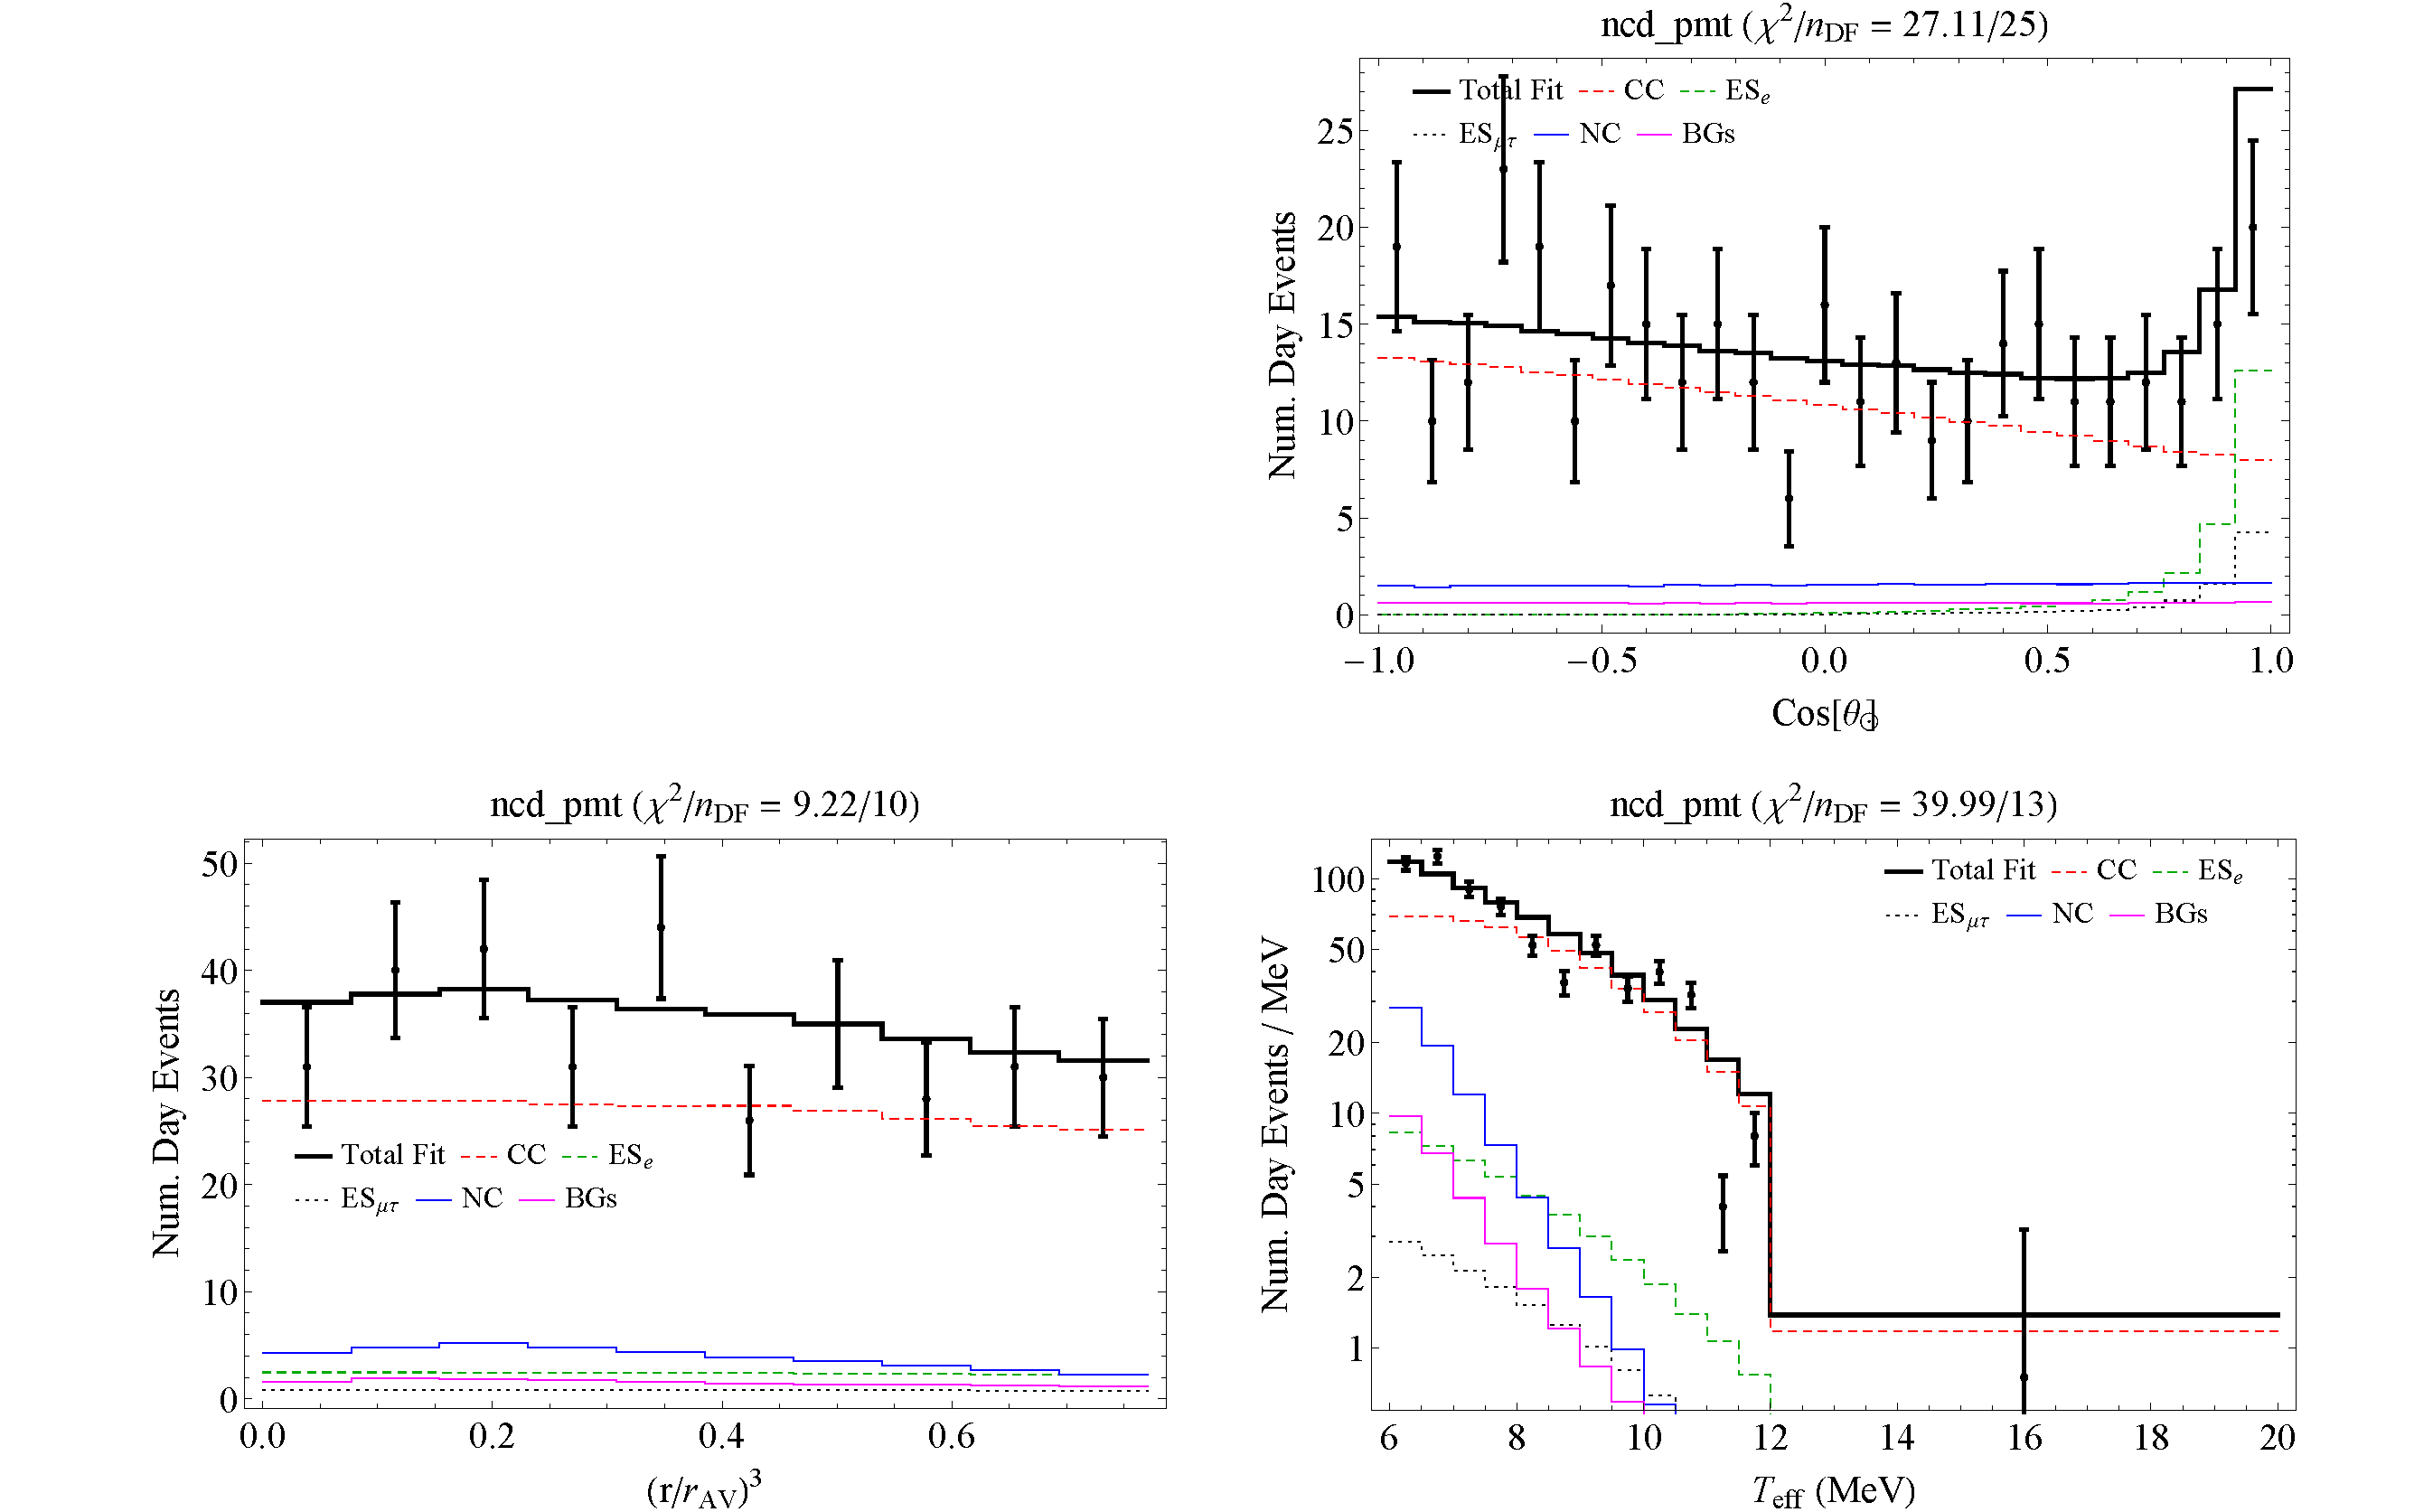
\includegraphics[width=0.95\columnwidth]{third_inf_ncd_pmt_day}
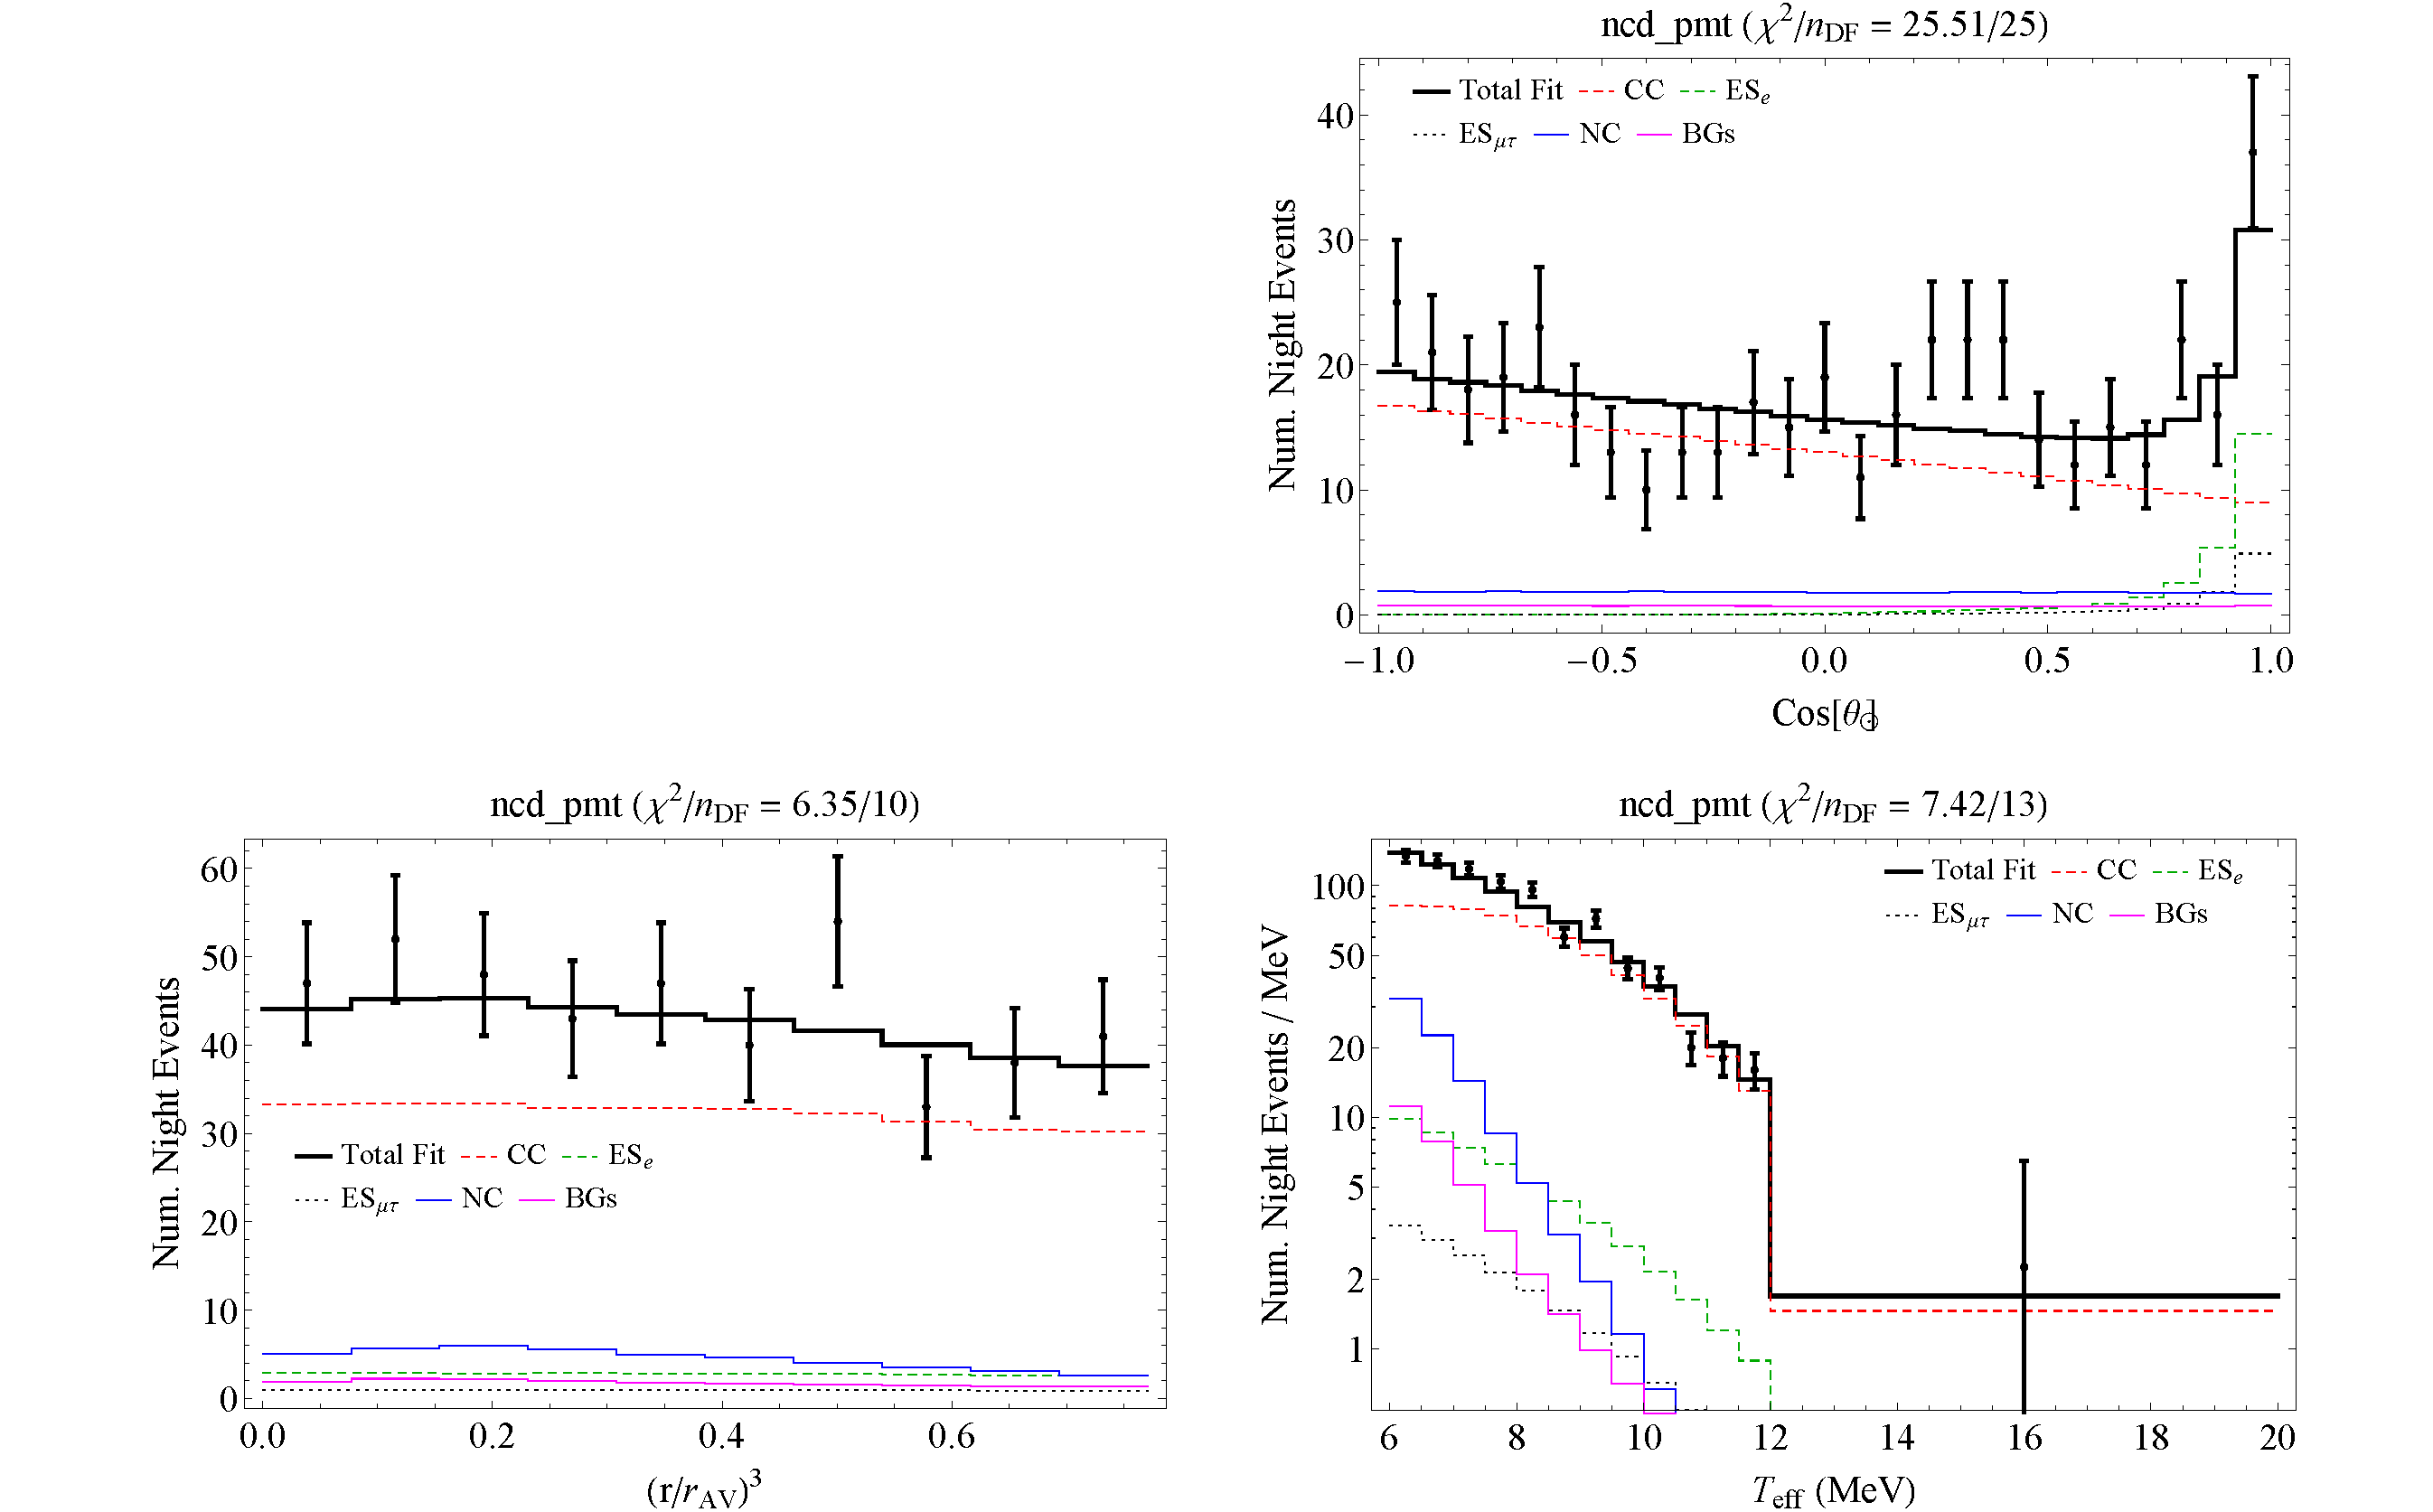
\includegraphics[width=0.95\columnwidth]{third_inf_ncd_pmt_night}
\caption{\label{fig:third_inf_ncd_pmt_obs}Observable distributions for Phase IIIb for the 1/3 dataset fit with $k_2$ fixed to infinity. Note that $\beta_{14}$ was not used in analyses for NCD phase.}
\end{figure}

\clearpage

\section{Final Fit}

\label{final_observables}

In the following sections are both the observables at the fit minimum and the observables for a more traditional no-decay scenario with $k_2$ fixed to infinity. Both cases for the full dataset.

\subsection{Fit Minimum}

Shown in \Cref{fig:final_d2o_obs,fig:final_salt_obs,fig:final_ncd_pmt_obs} are the observable distributions for a 3 phase fit to full dataset as described in \Cref{final}.

\begin{figure}
\centering
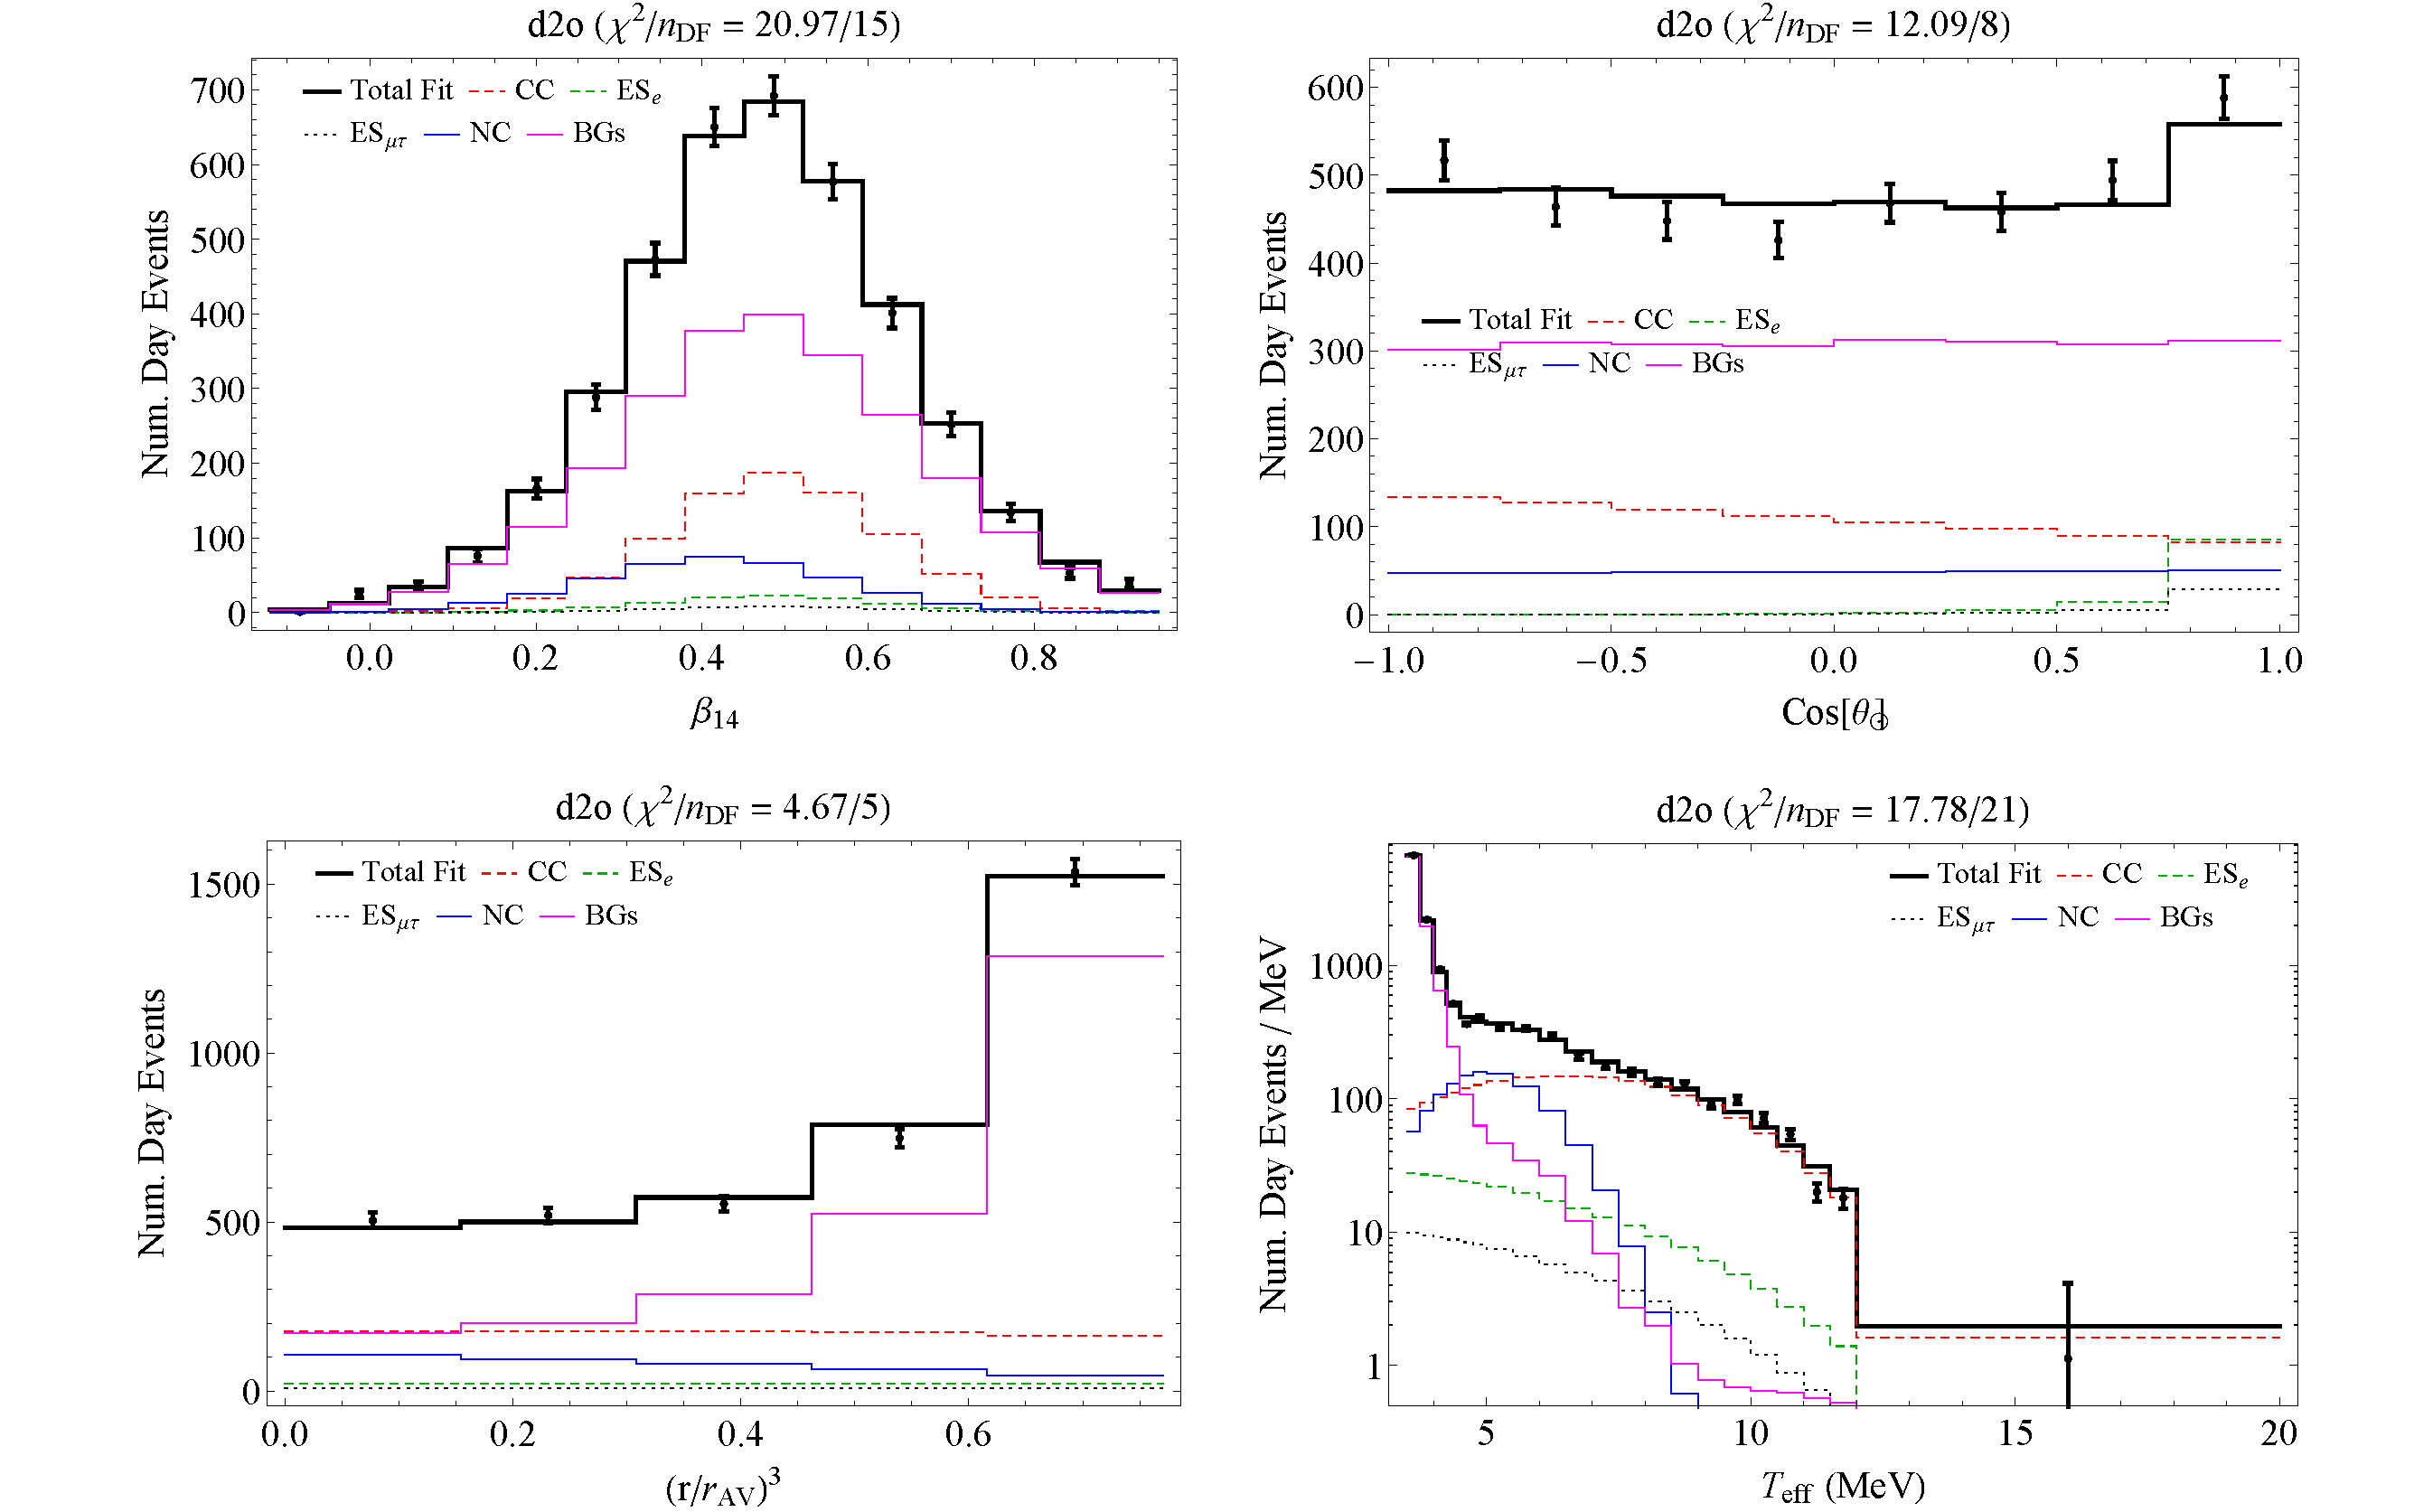
\includegraphics[width=0.95\columnwidth]{final_min_d2o_day}
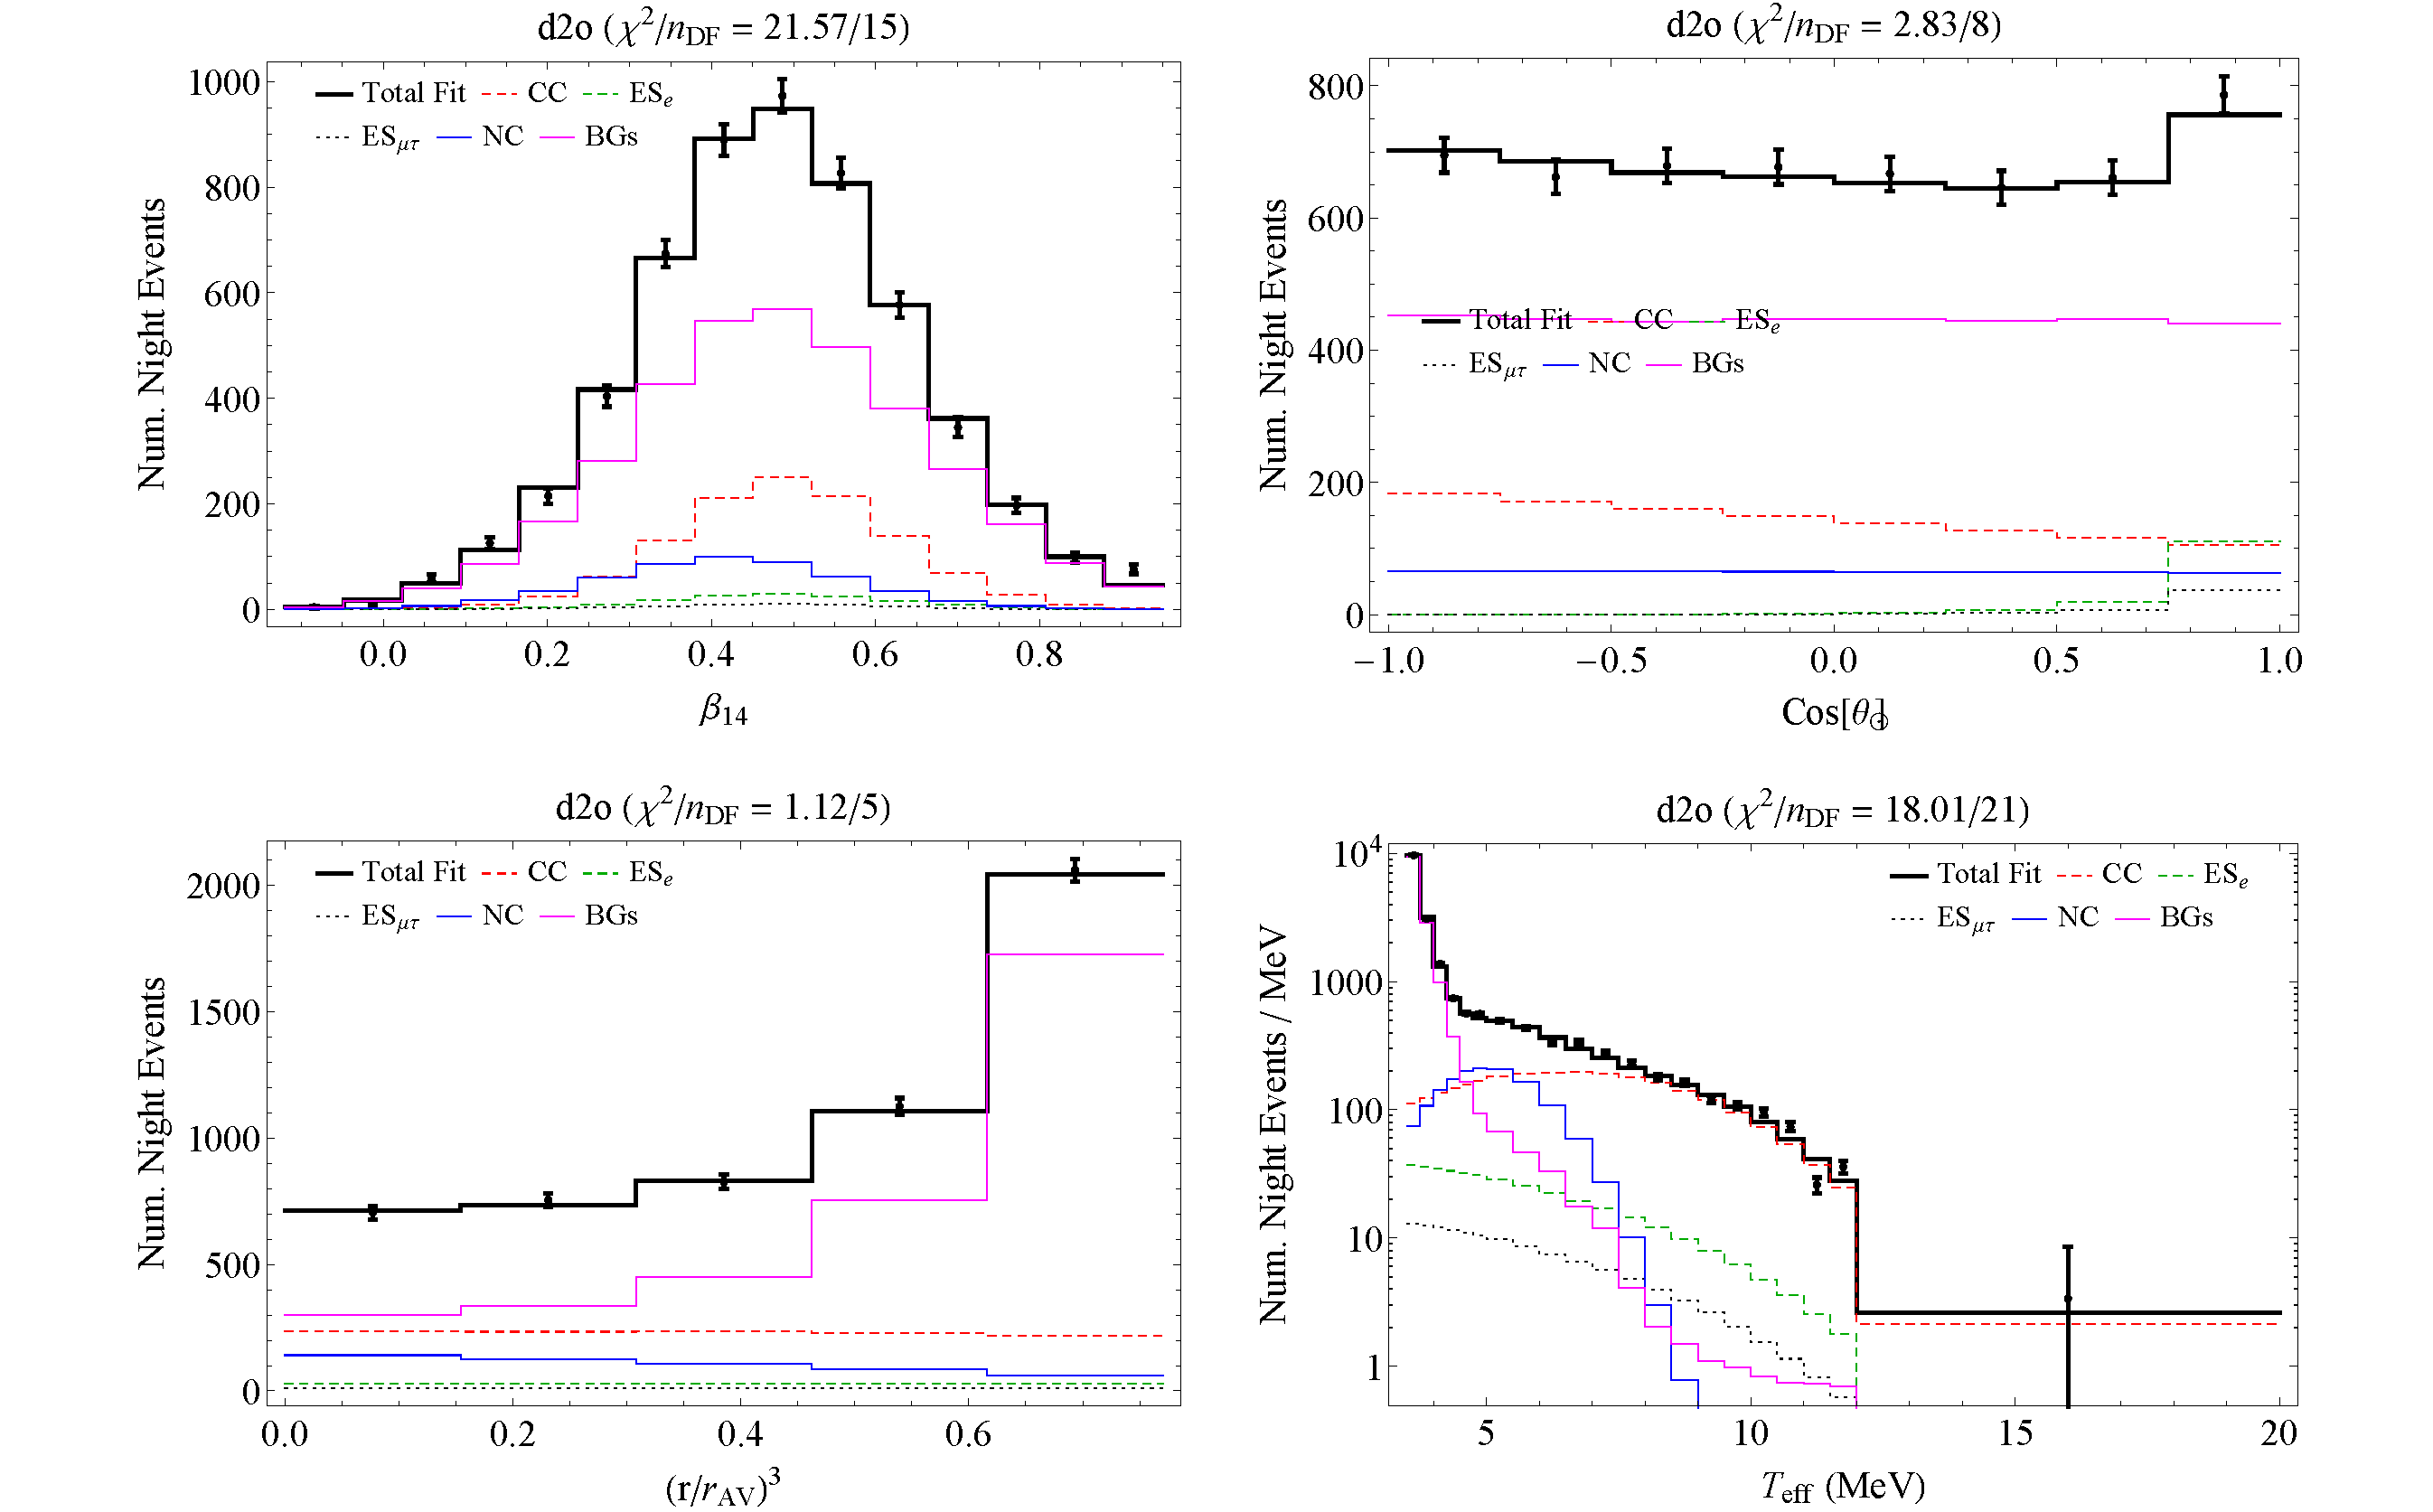
\includegraphics[width=0.95\columnwidth]{final_min_d2o_night}
\caption{\label{fig:final_d2o_obs}Observable distributions for Phase I for the final fit.}
\end{figure}
\begin{figure}
\centering
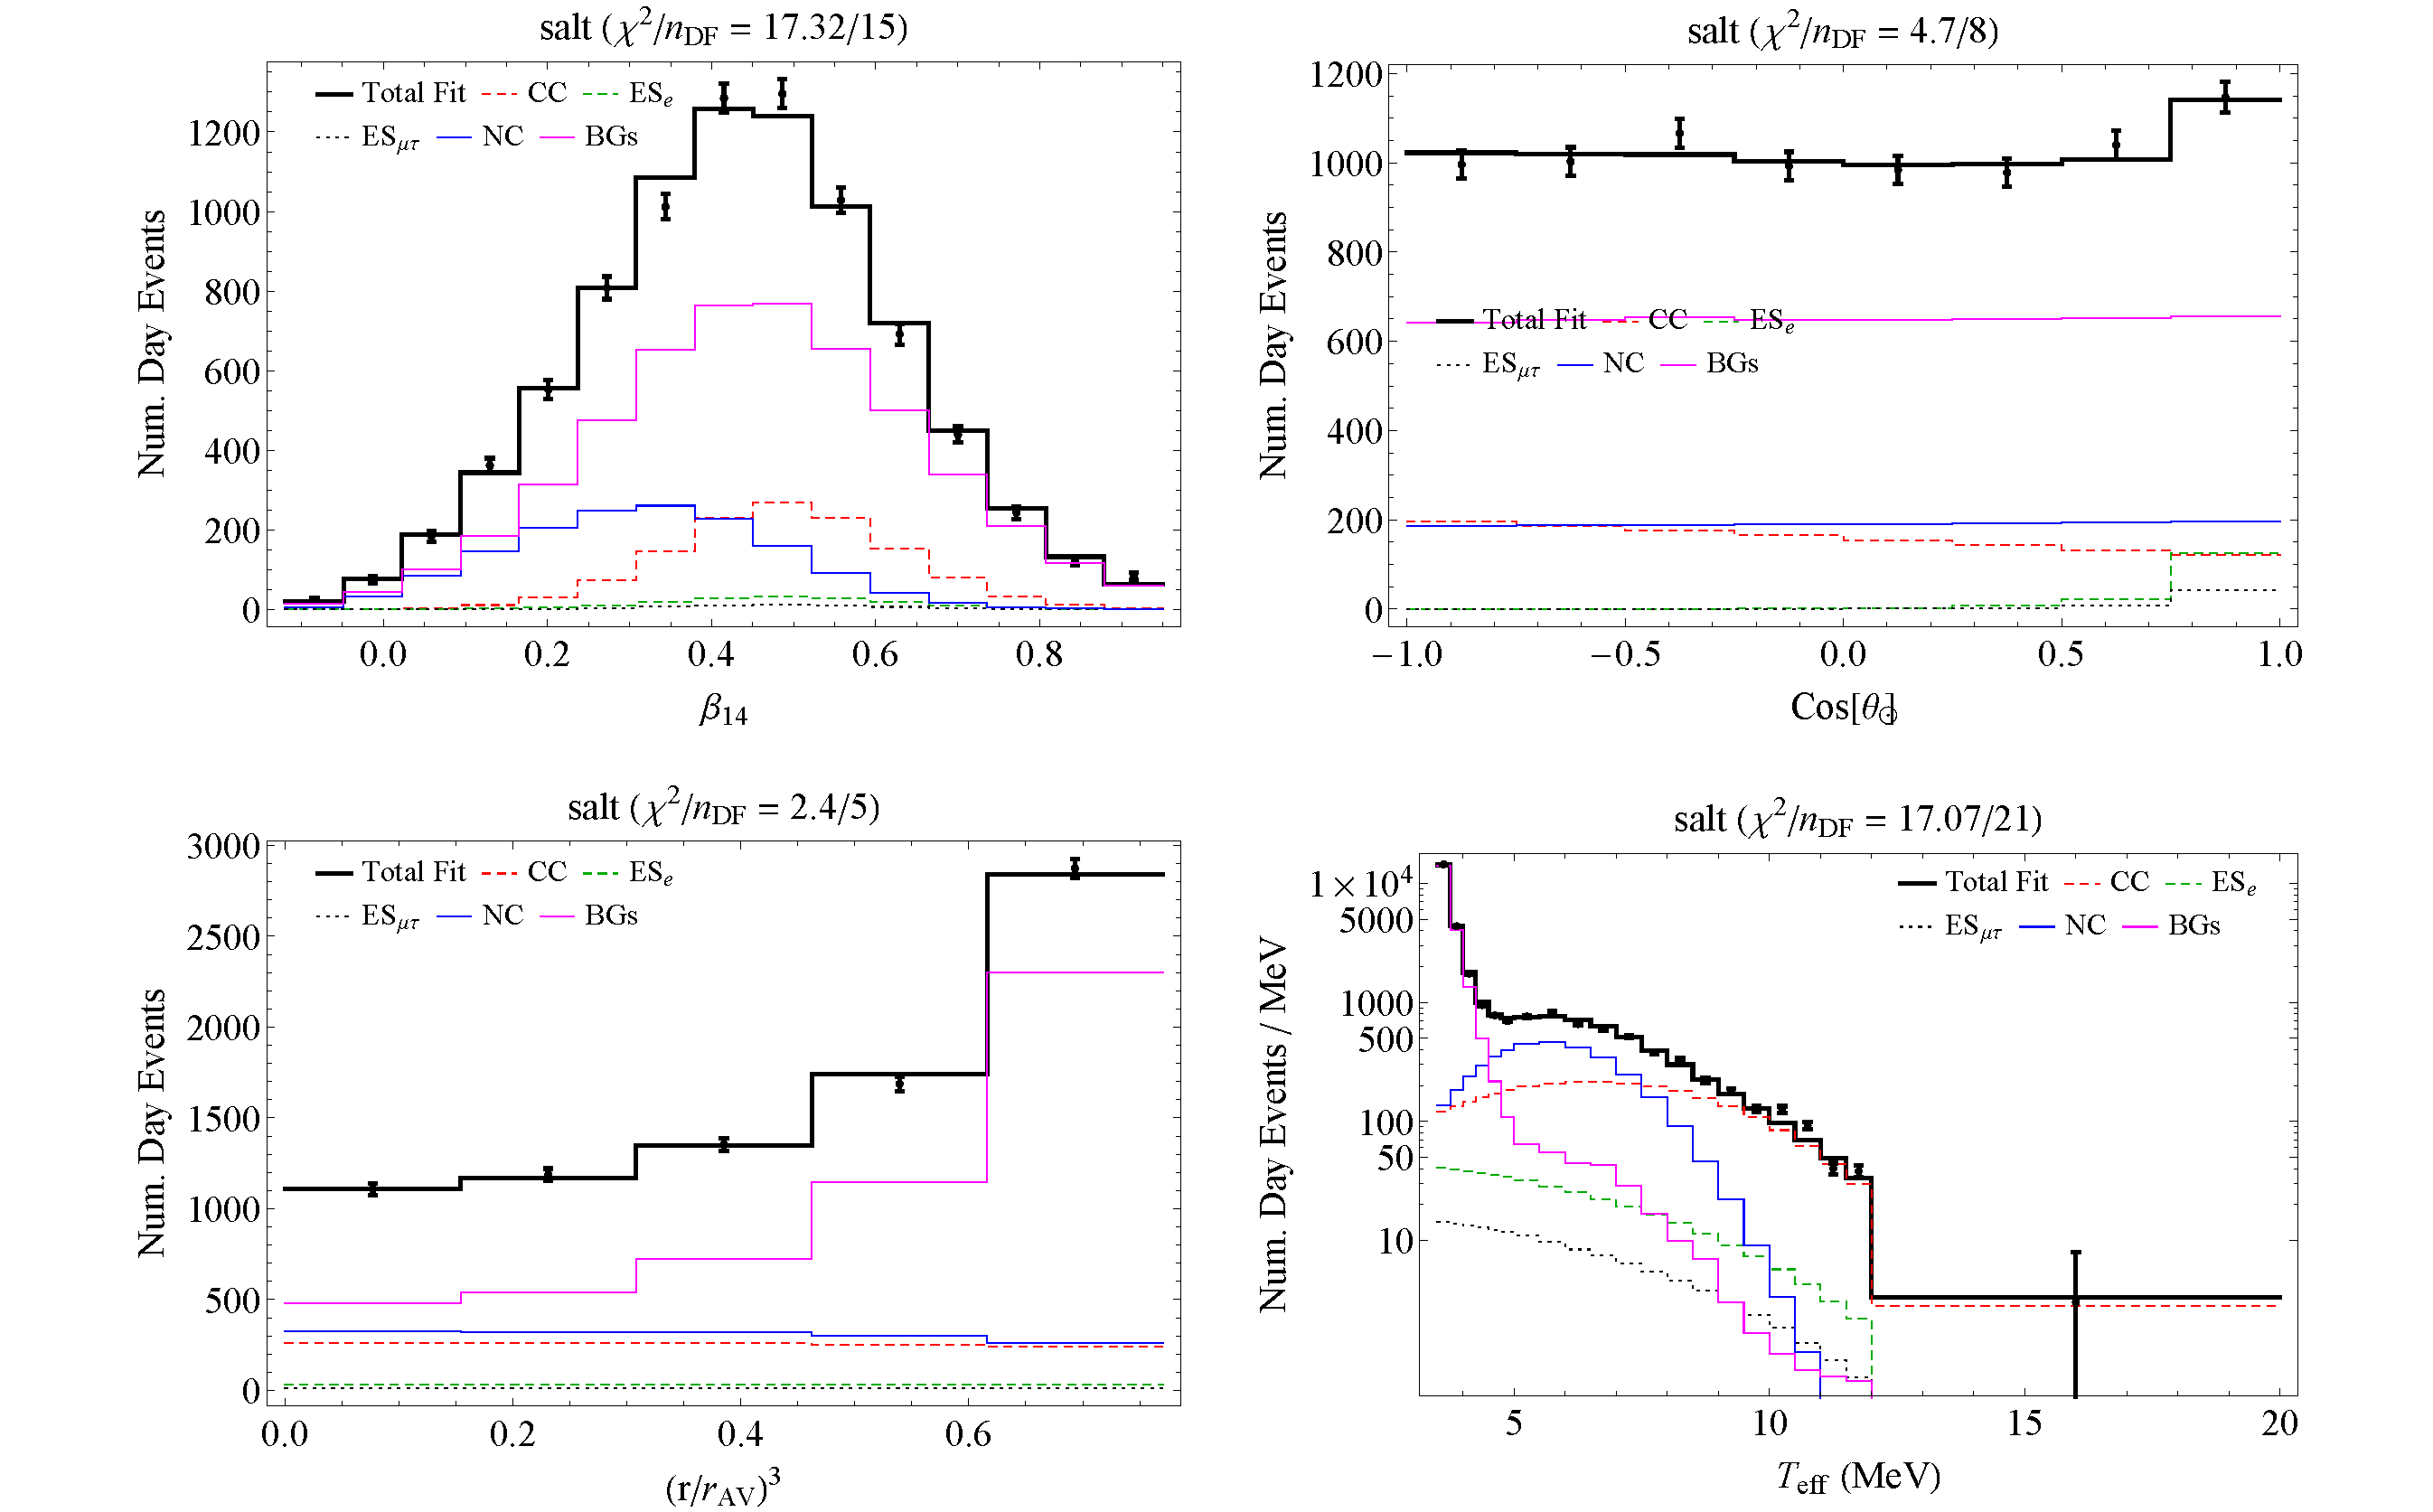
\includegraphics[width=0.95\columnwidth]{final_min_salt_day}
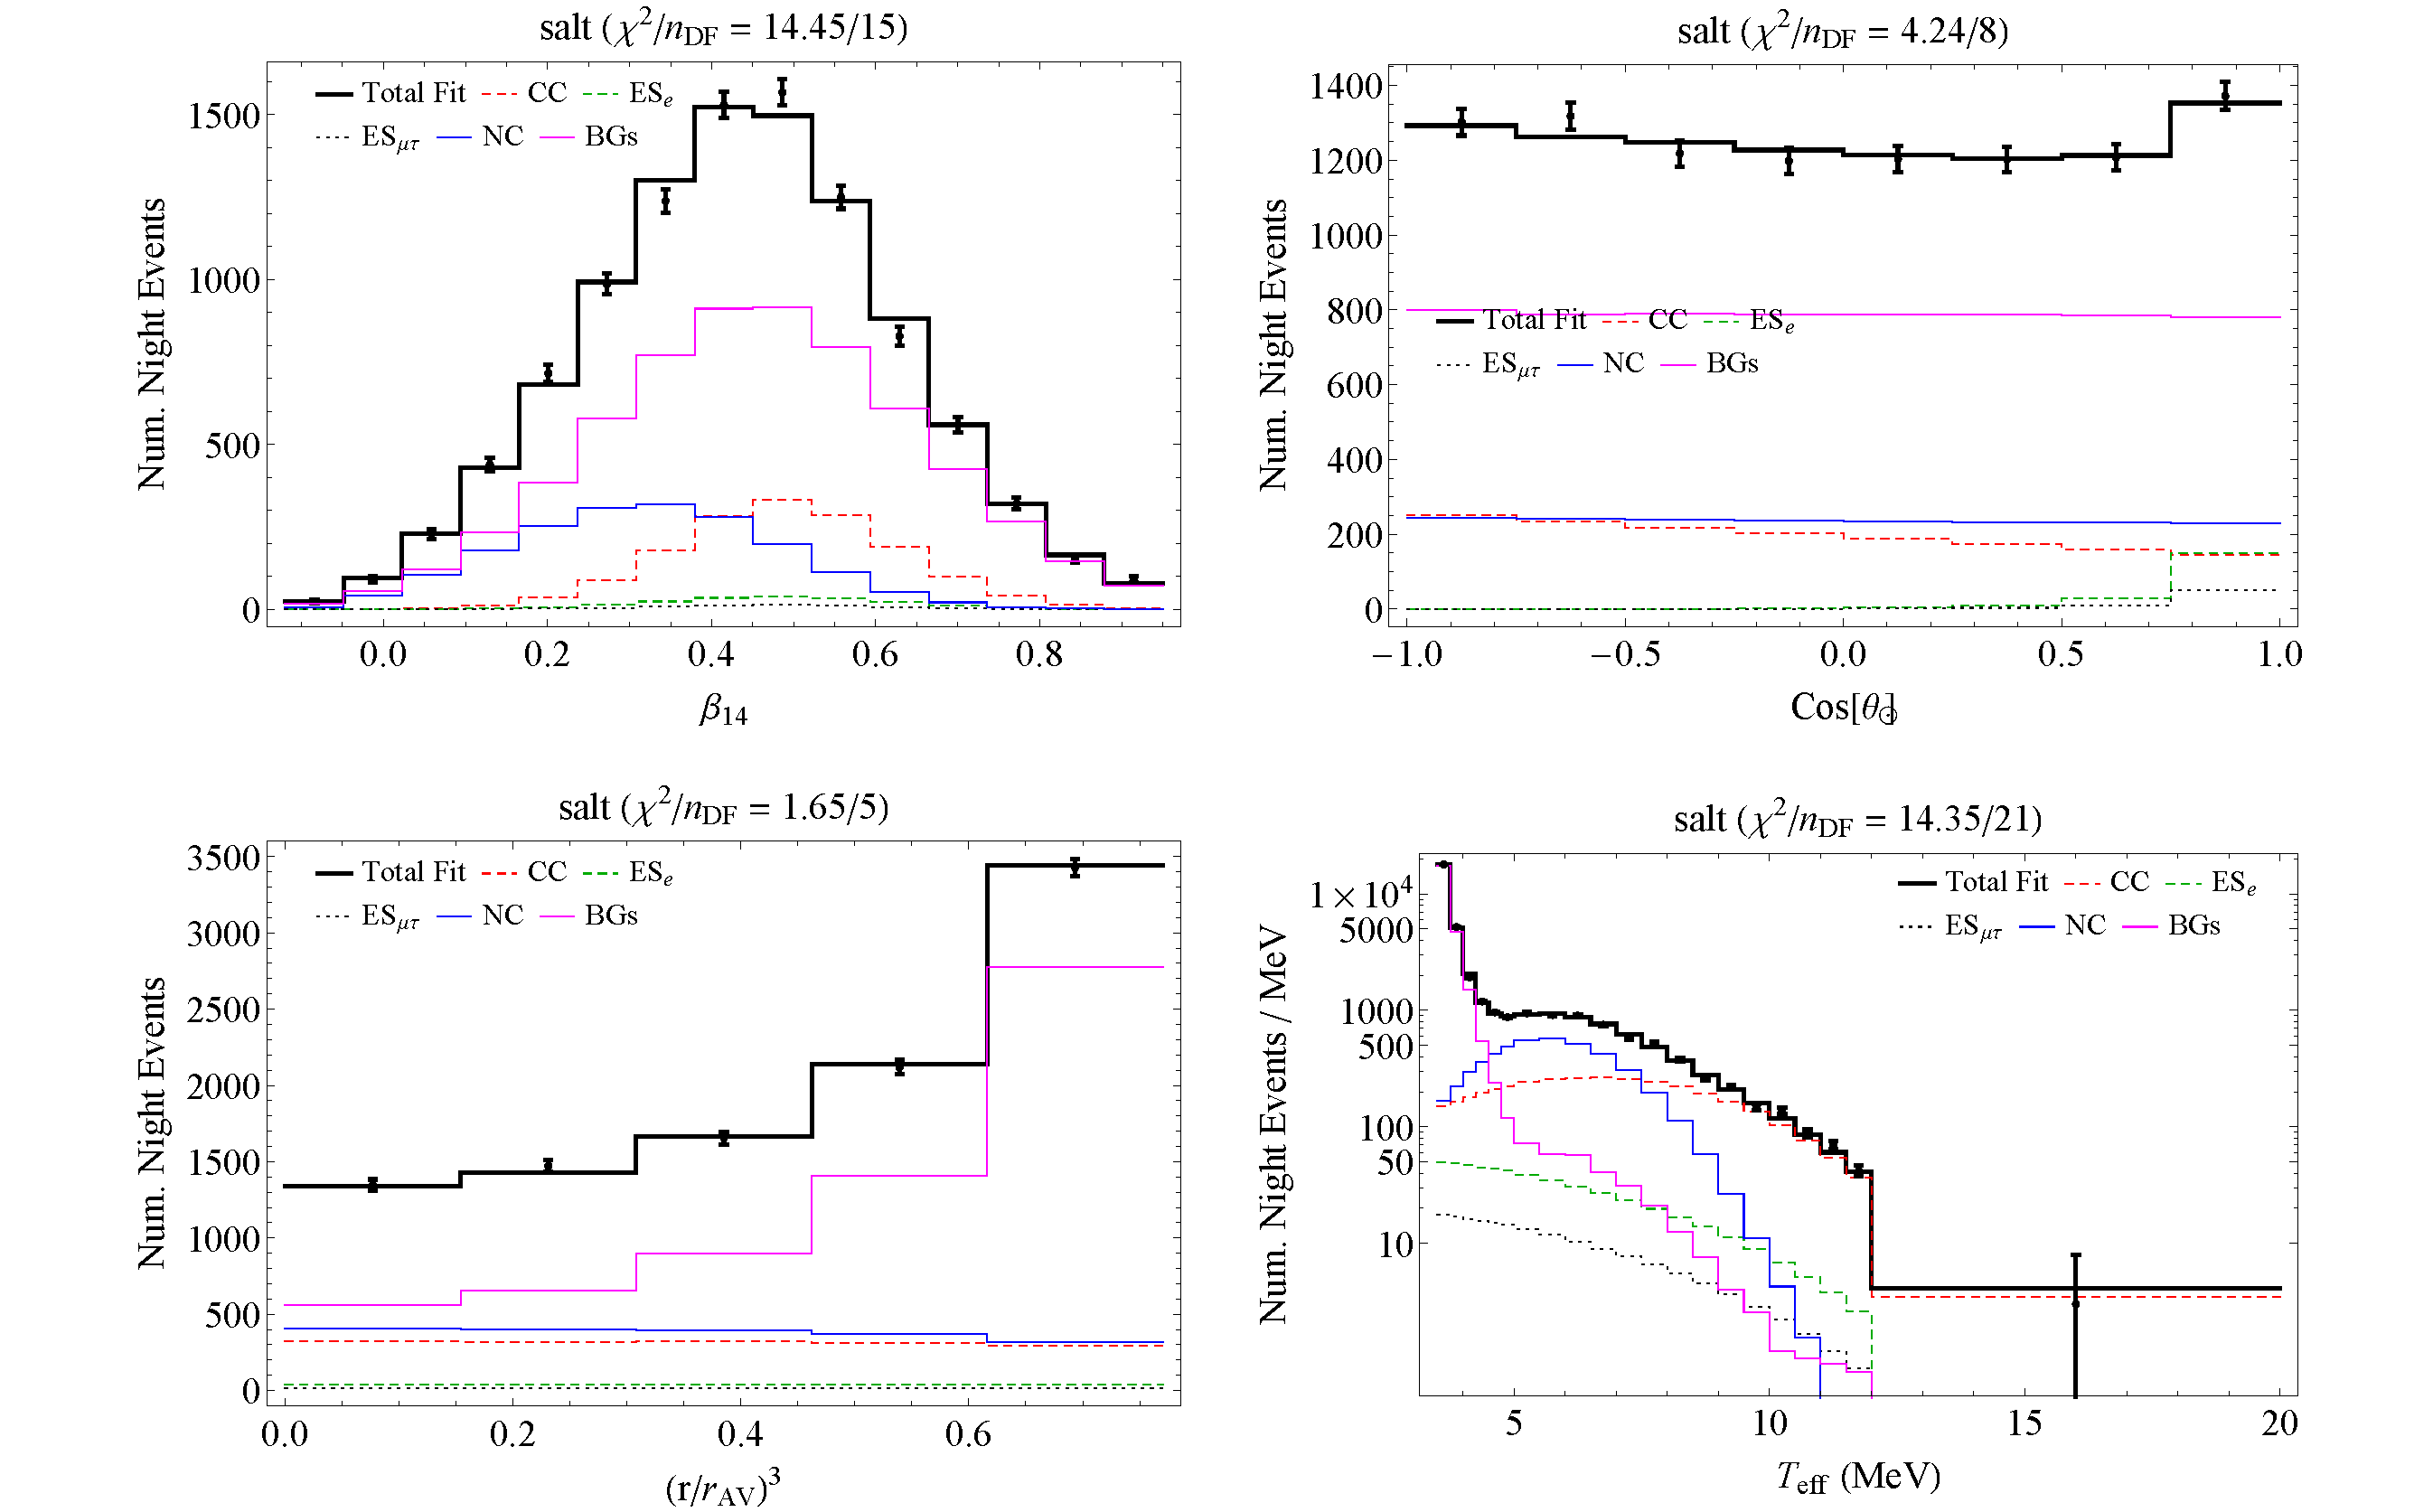
\includegraphics[width=0.95\columnwidth]{final_min_salt_night}
\caption{\label{fig:final_salt_obs}Observable distributions for Phase II for the final fit.}
\end{figure}
\begin{figure}
\centering
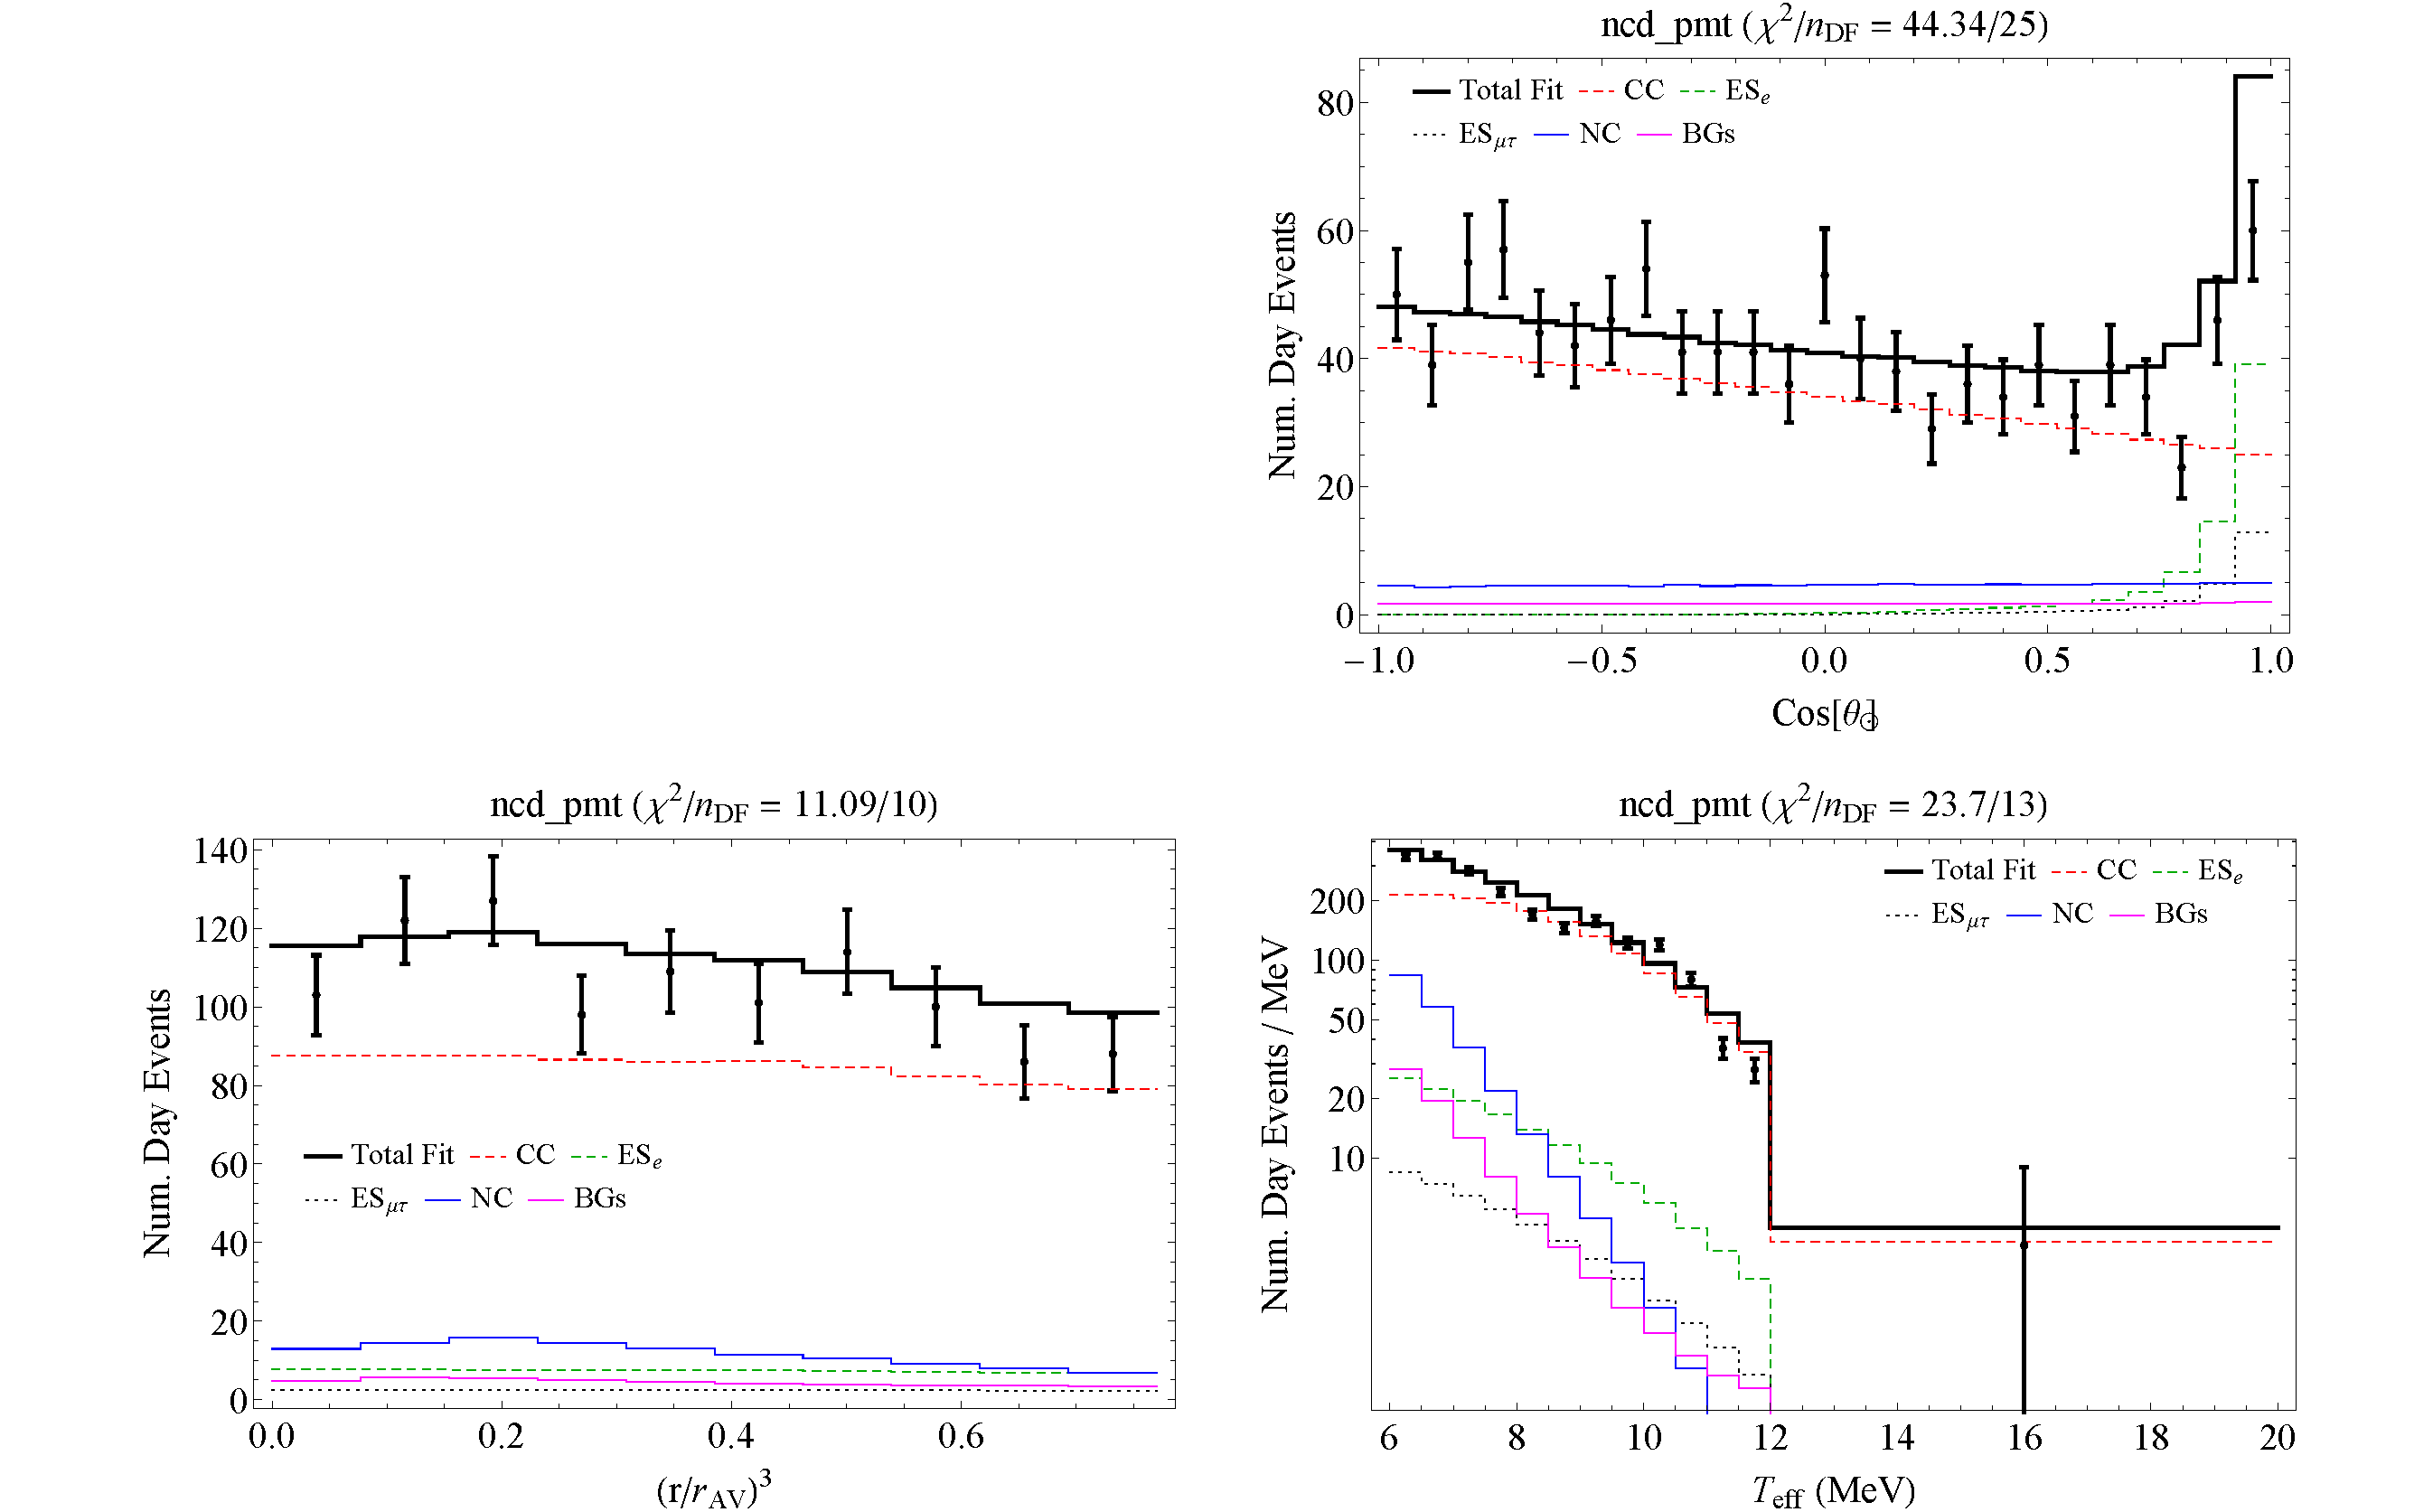
\includegraphics[width=0.95\columnwidth]{final_min_ncd_pmt_day}
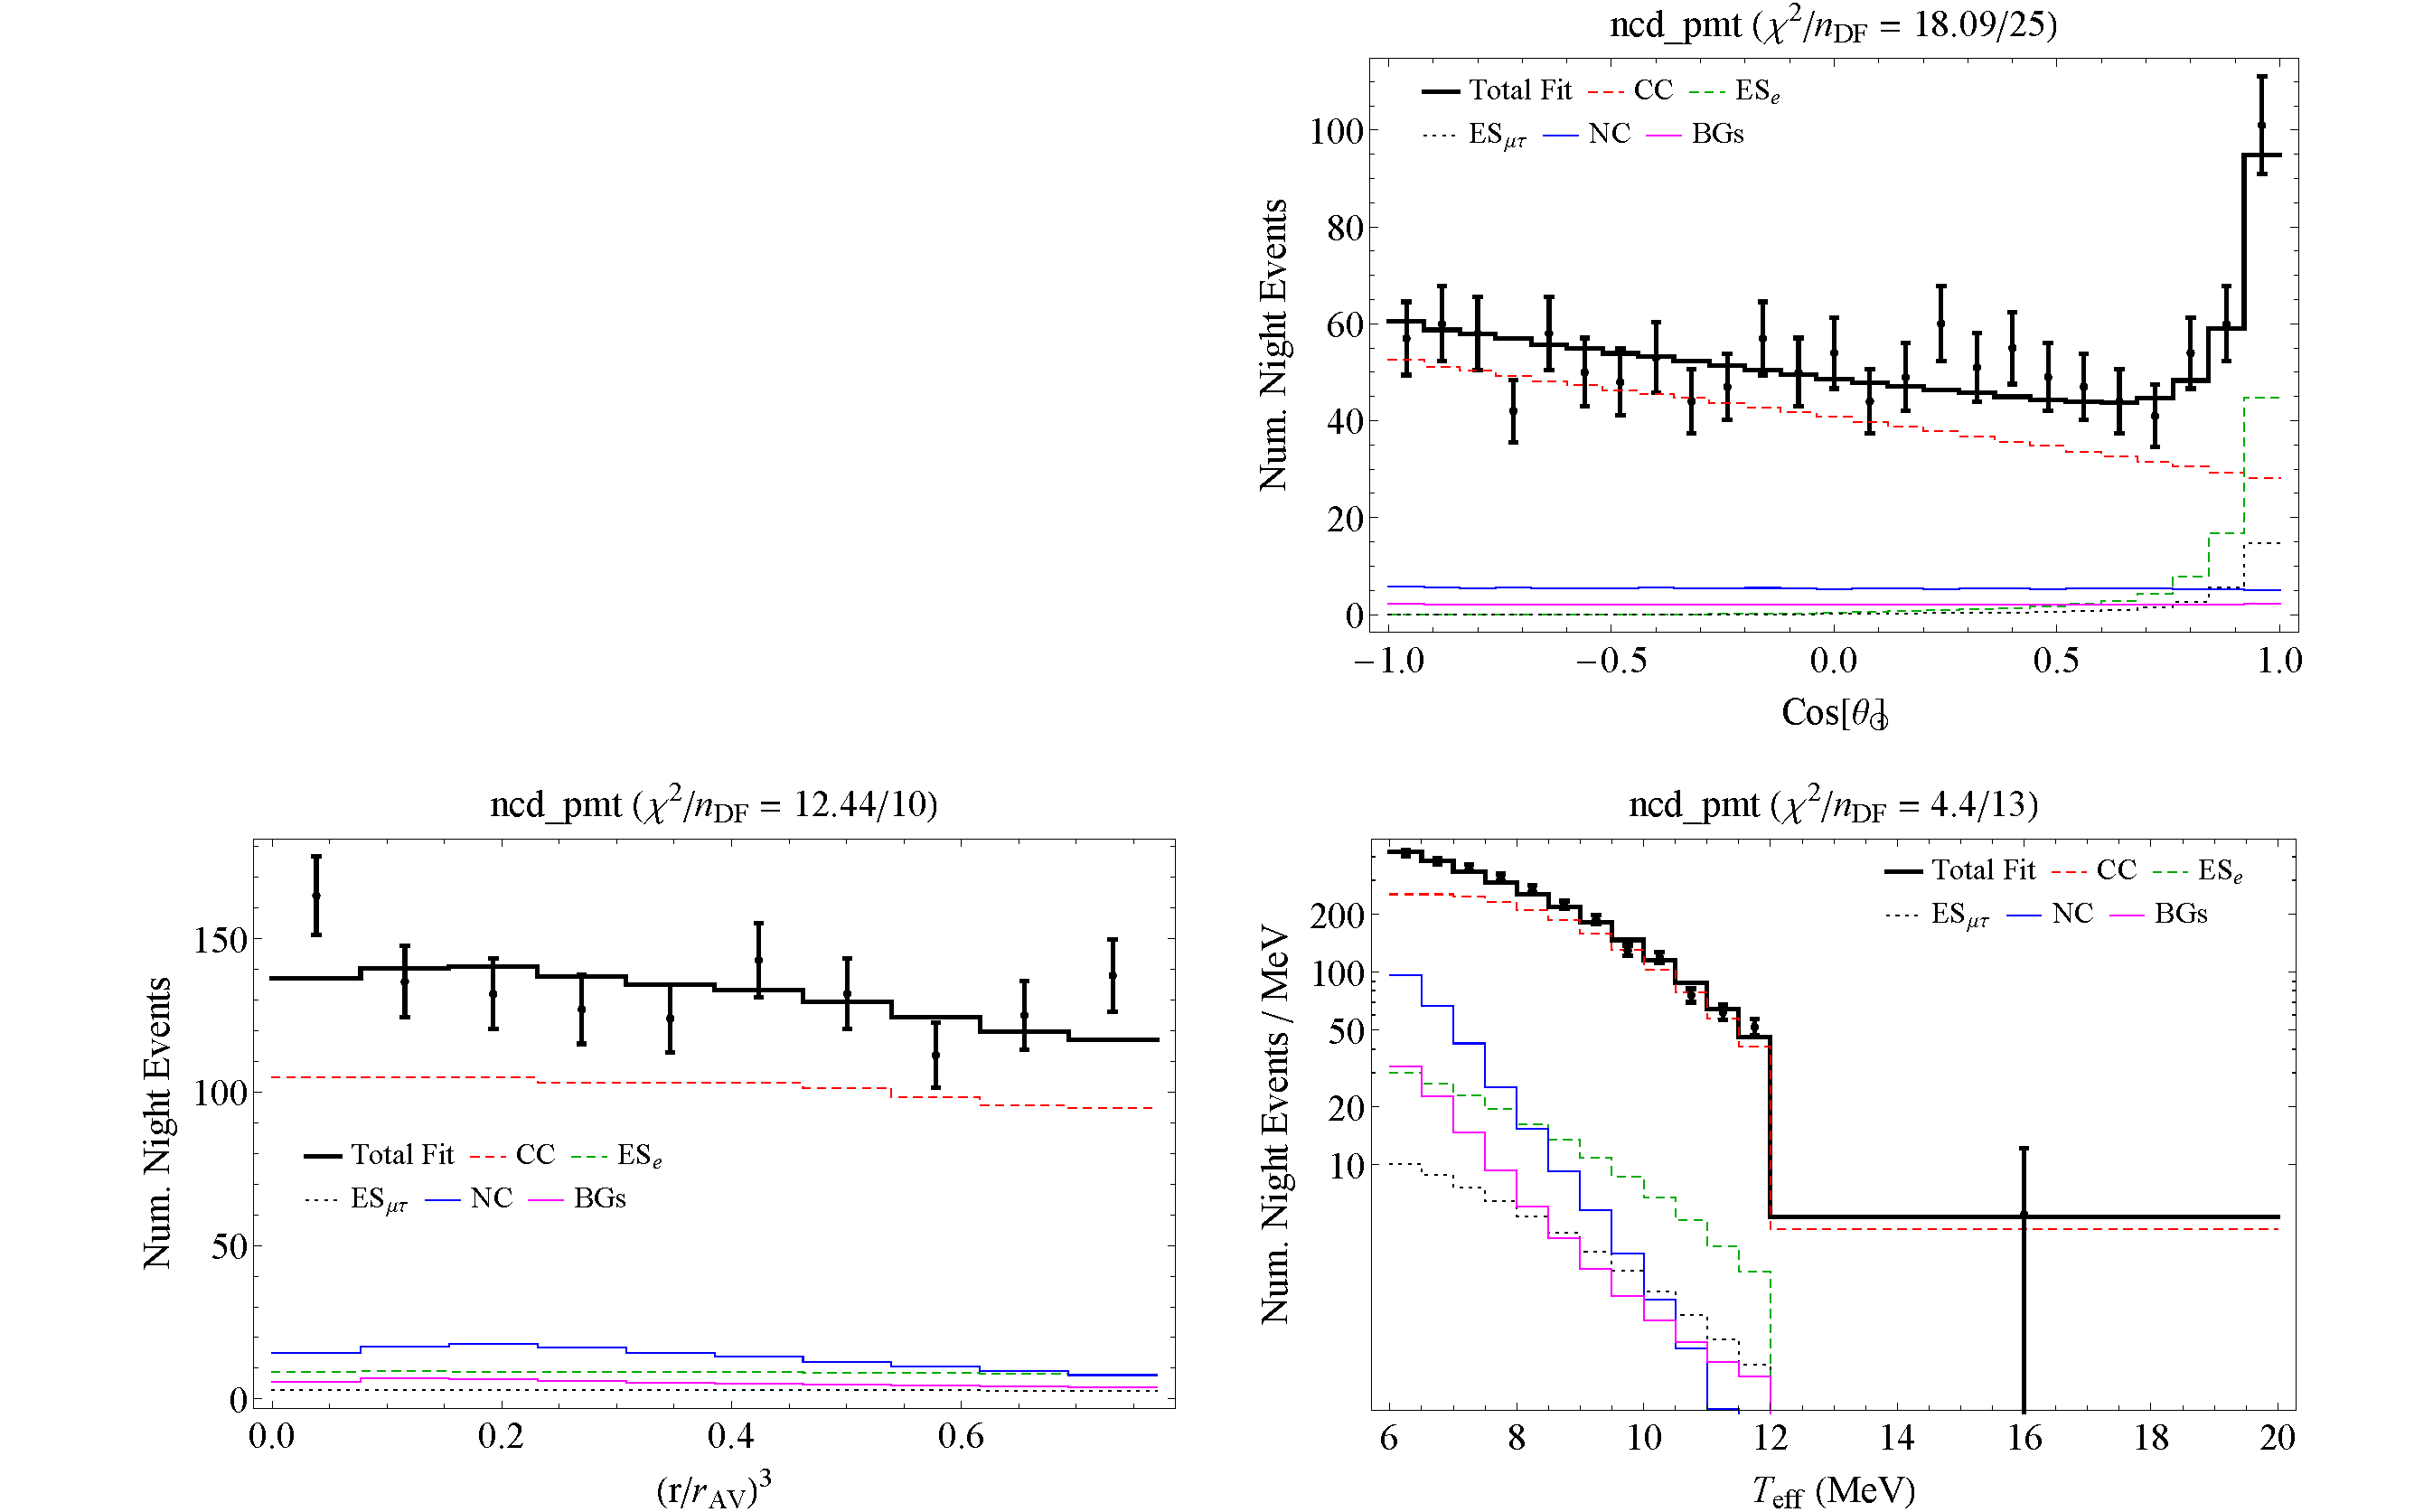
\includegraphics[width=0.95\columnwidth]{final_min_ncd_pmt_night}
\caption{\label{fig:final_ncd_pmt_obs}Observable distributions for Phase IIIb for the final fit. Note that $\beta_{14}$ was not used in analyses for NCD phase.}
\end{figure}

\clearpage

\subsection{\texorpdfstring{$k_2$}{k2} Fixed to Infinity}

Shown in \Cref{fig:final_inf_d2o_obs,fig:final_inf_salt_obs,fig:final_inf_ncd_pmt_obs} are the observable distributions for a 3 phase fit to the full dataset with no decay ($k_2$ fixed at infinity). These plots are provided primarily as a cross check.

\begin{figure}
\centering
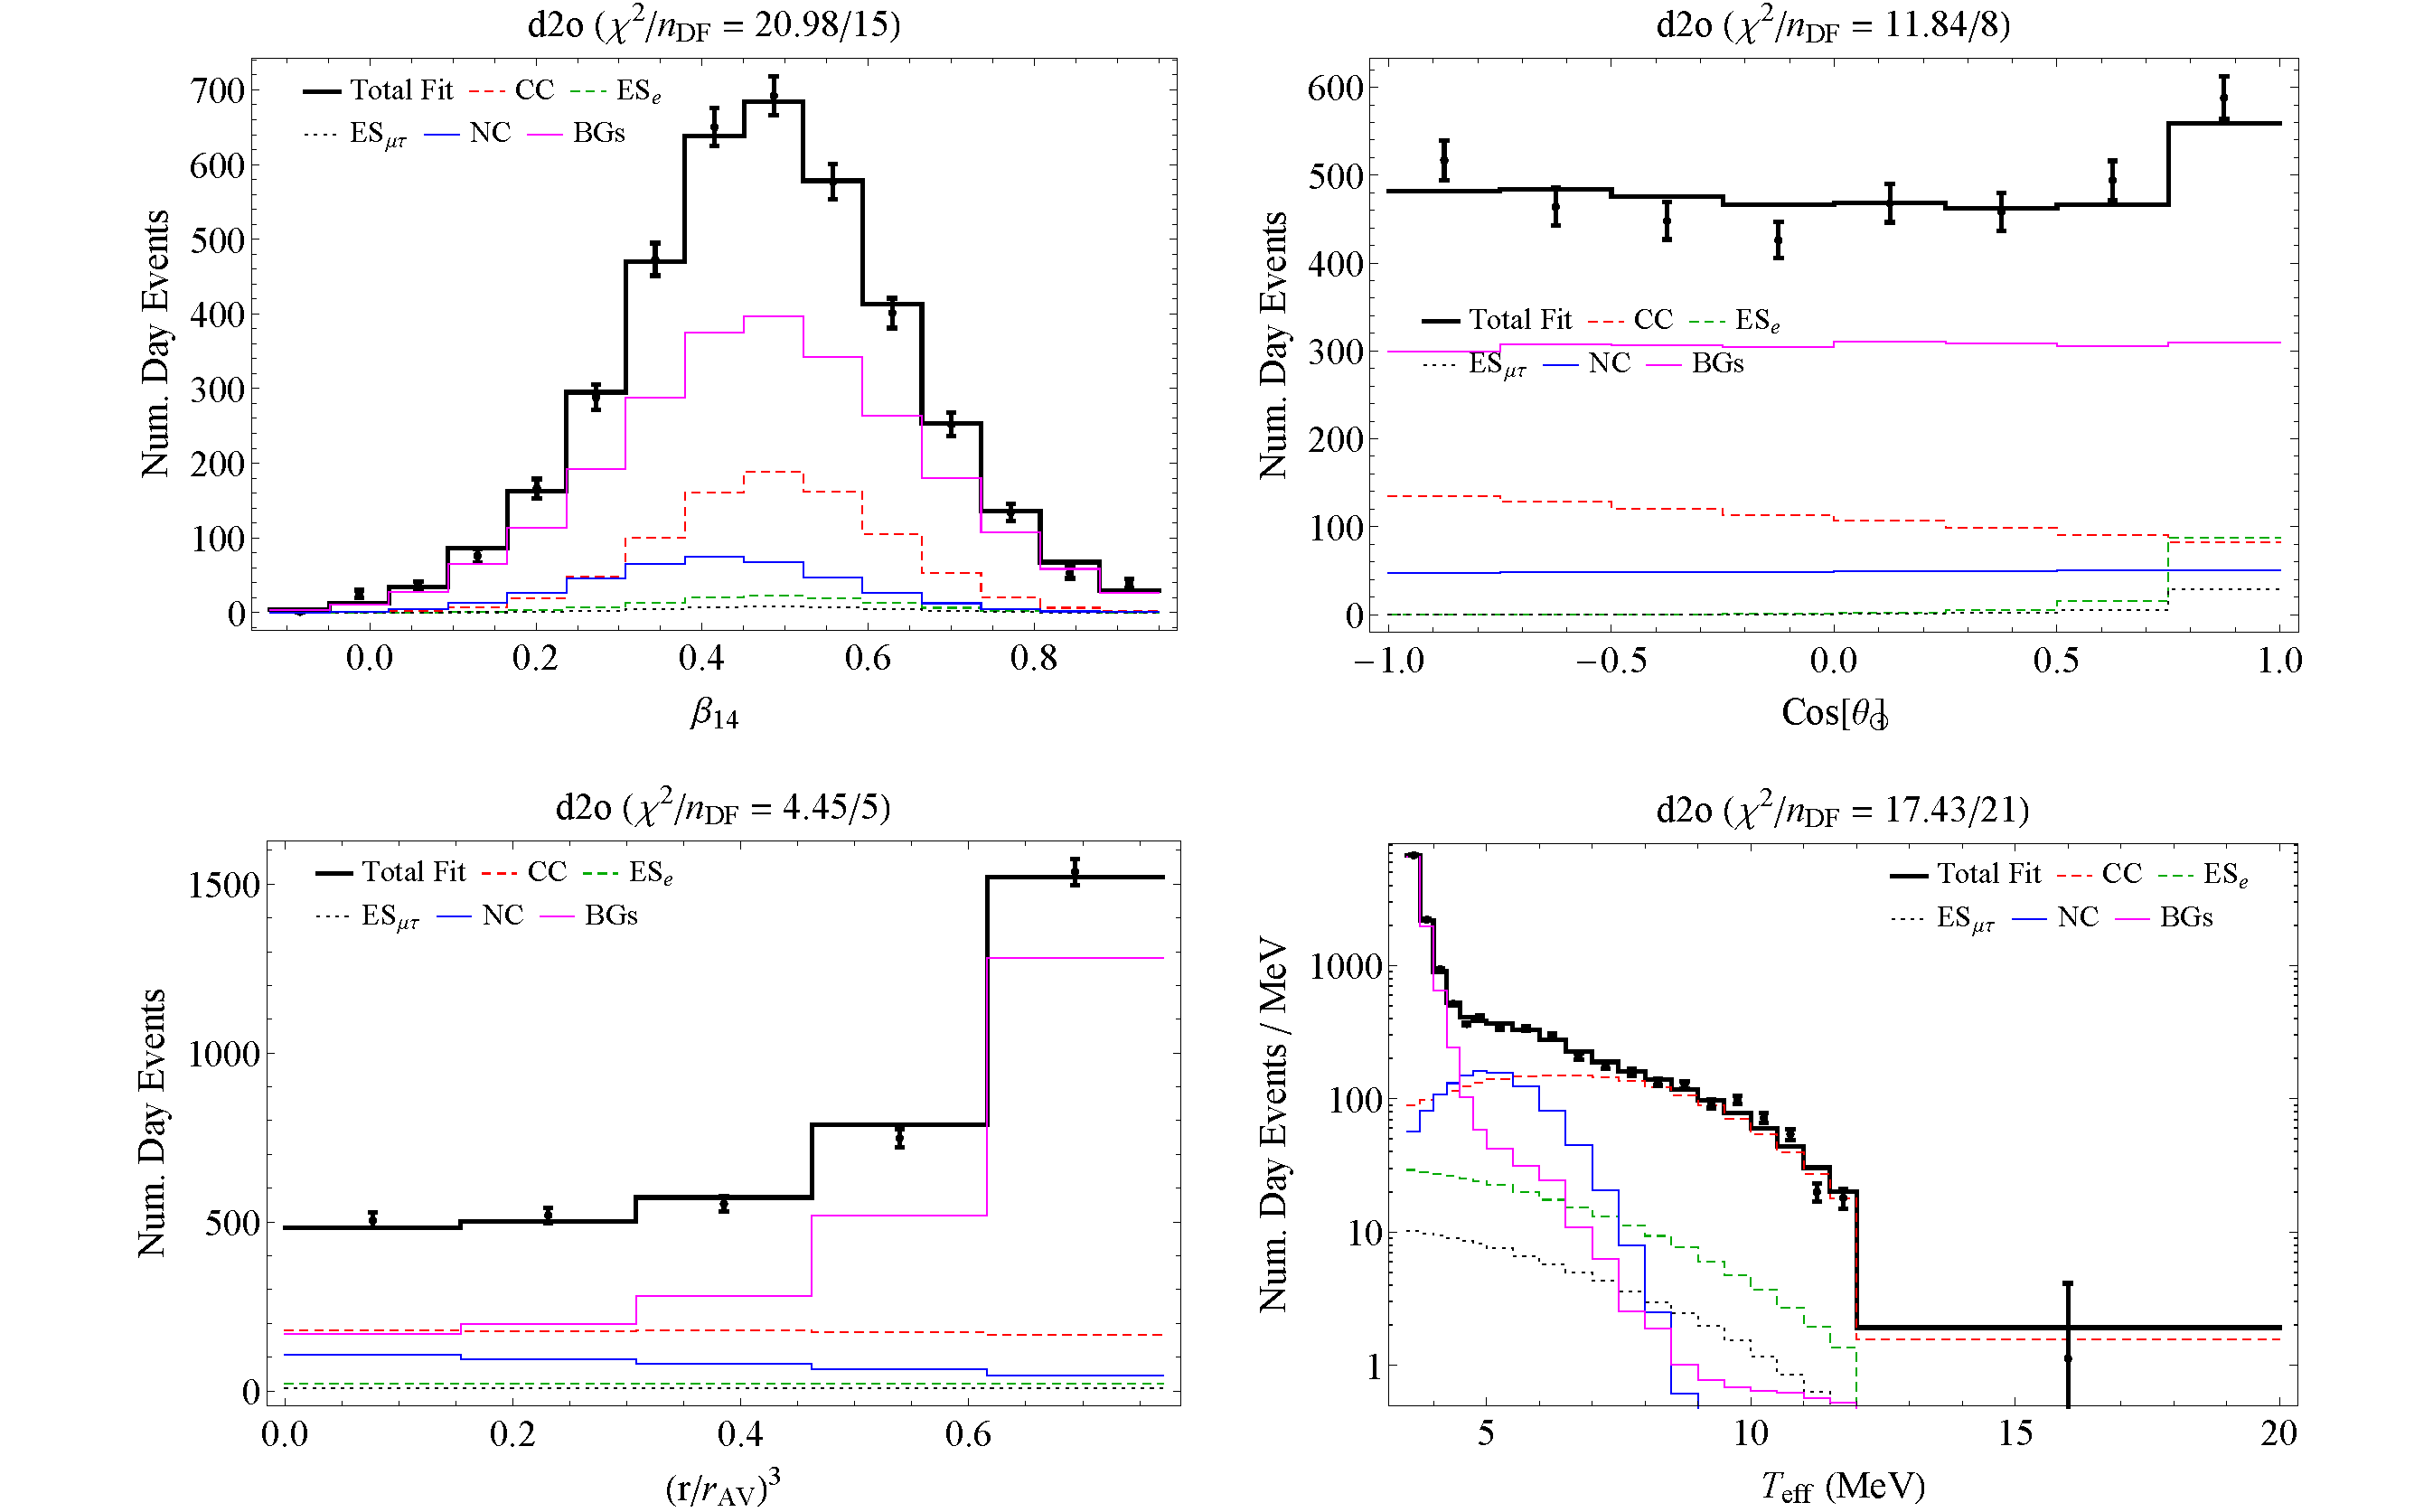
\includegraphics[width=0.95\columnwidth]{final_inf_d2o_day}
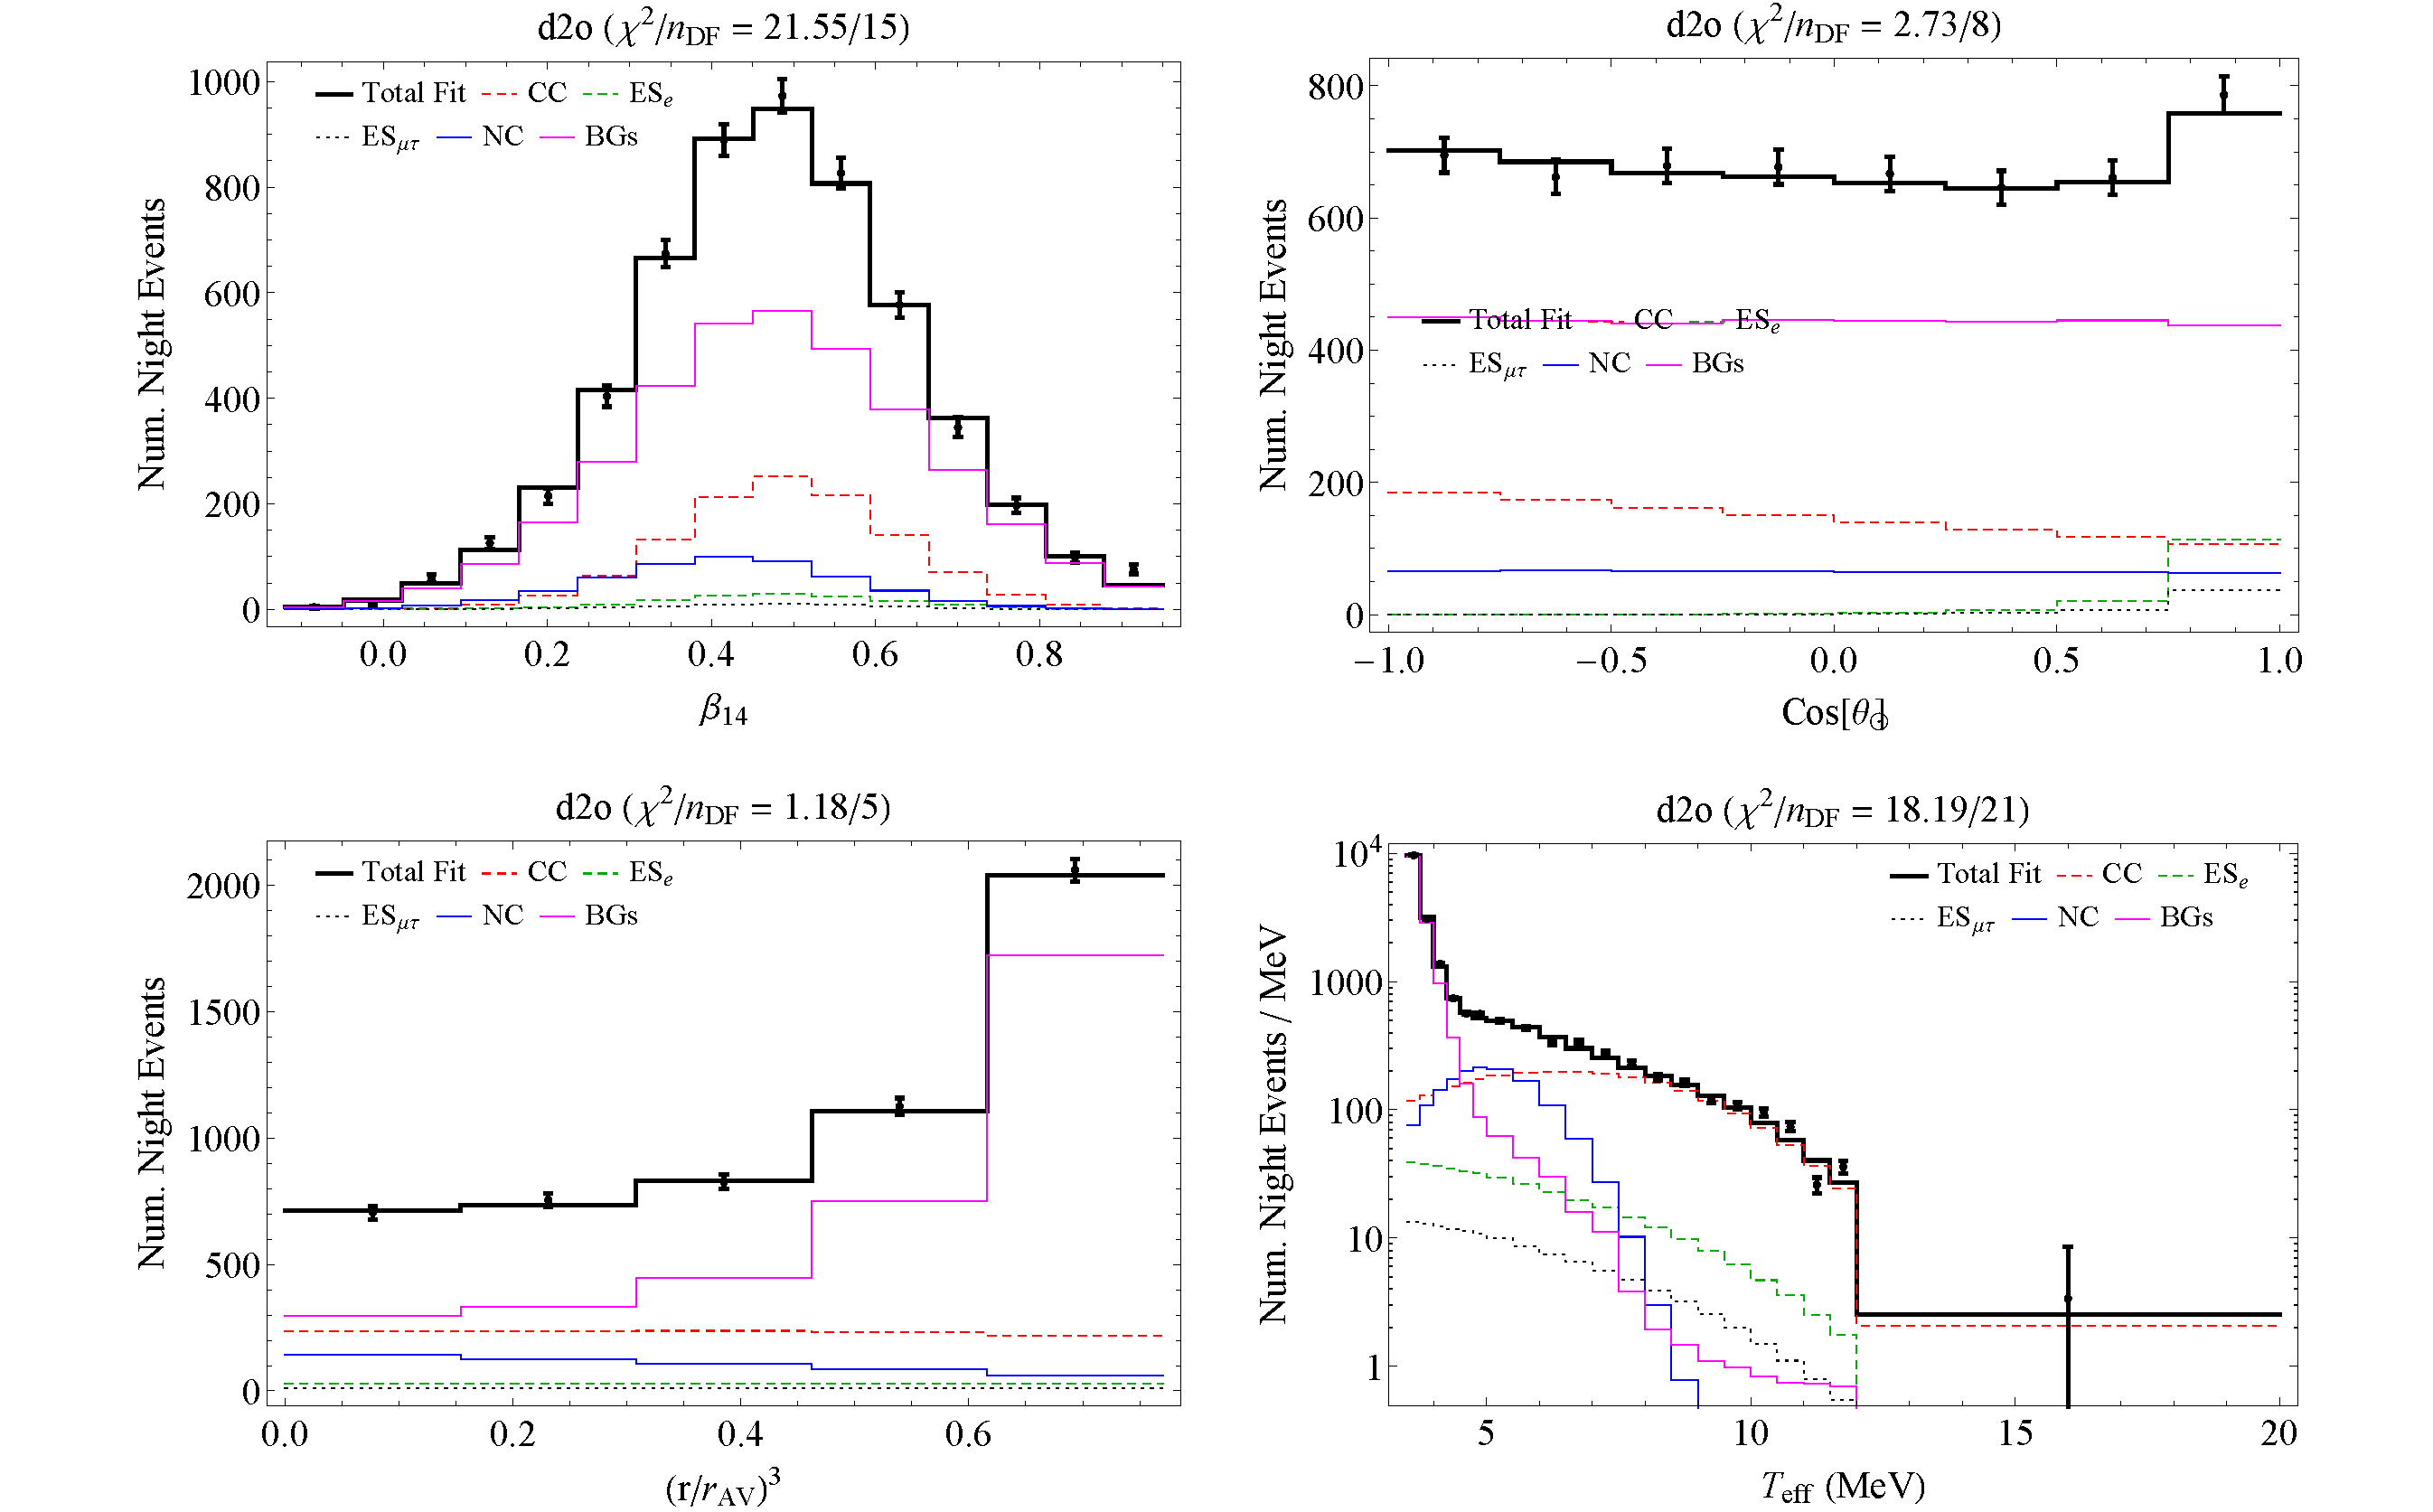
\includegraphics[width=0.95\columnwidth]{final_inf_d2o_night}
\caption{\label{fig:final_inf_d2o_obs}Observable distributions for Phase I for the final fit with $k_2$ fixed to infinity.}
\end{figure}
\begin{figure}
\centering
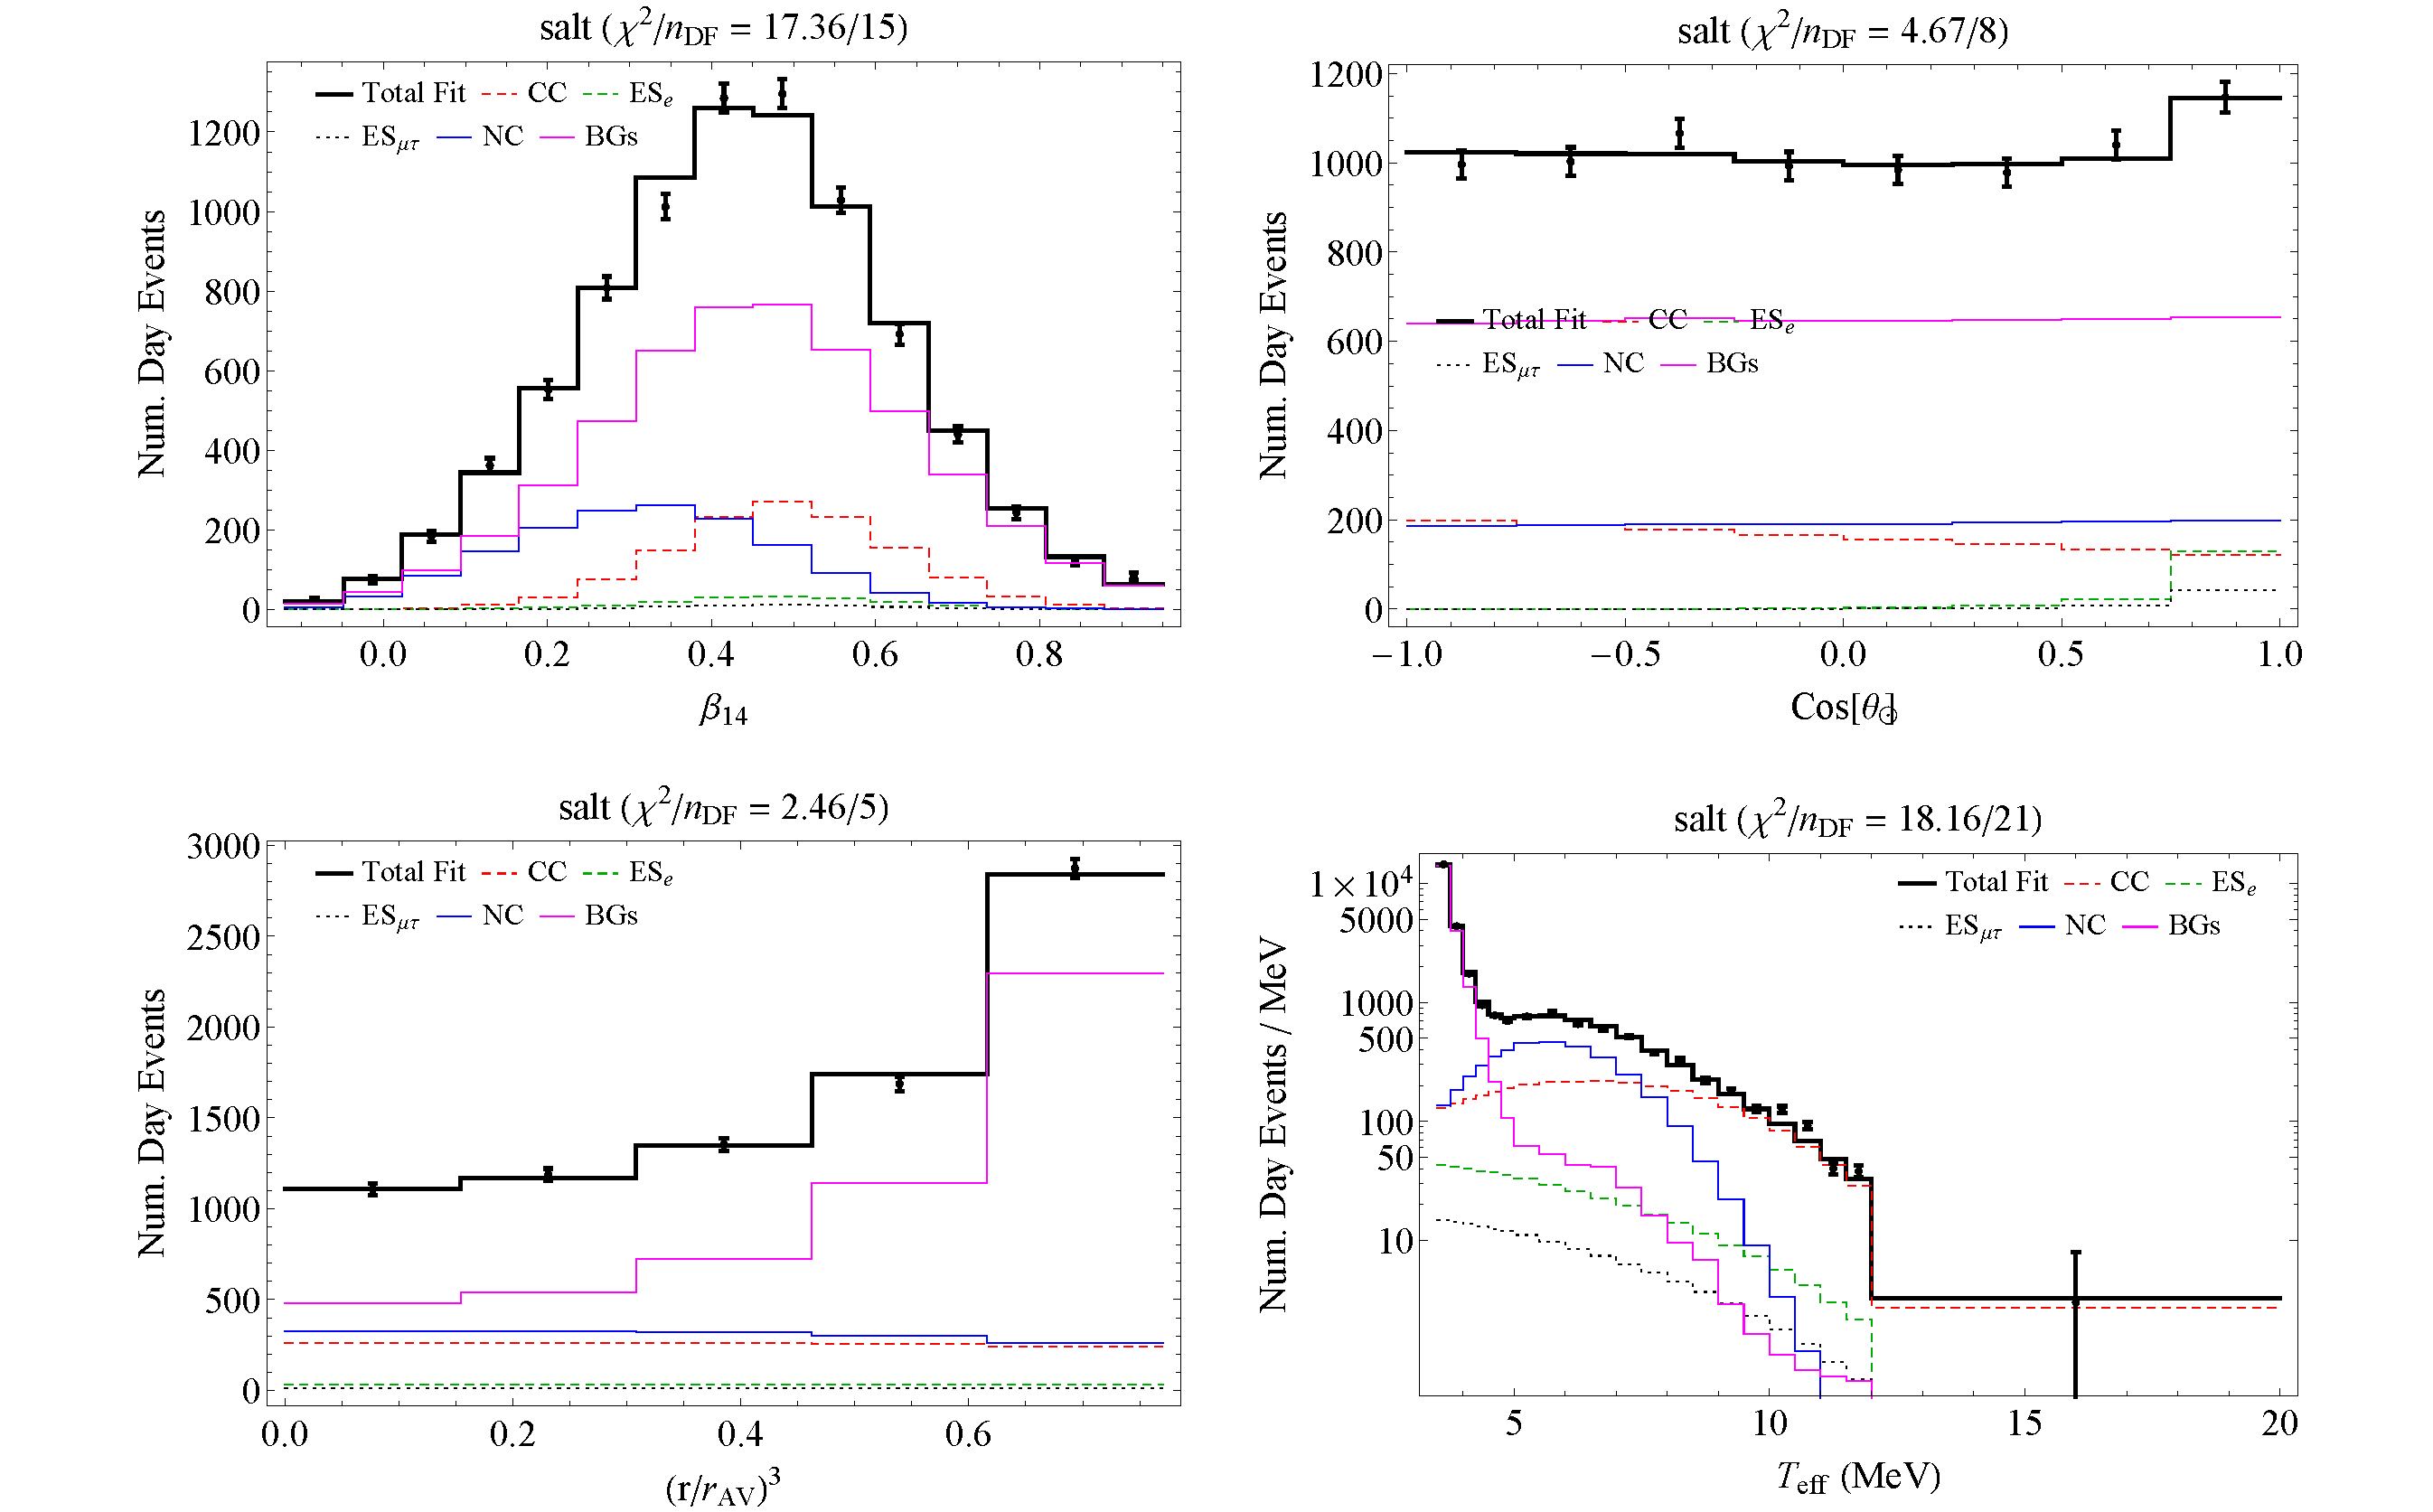
\includegraphics[width=0.95\columnwidth]{final_inf_salt_day}
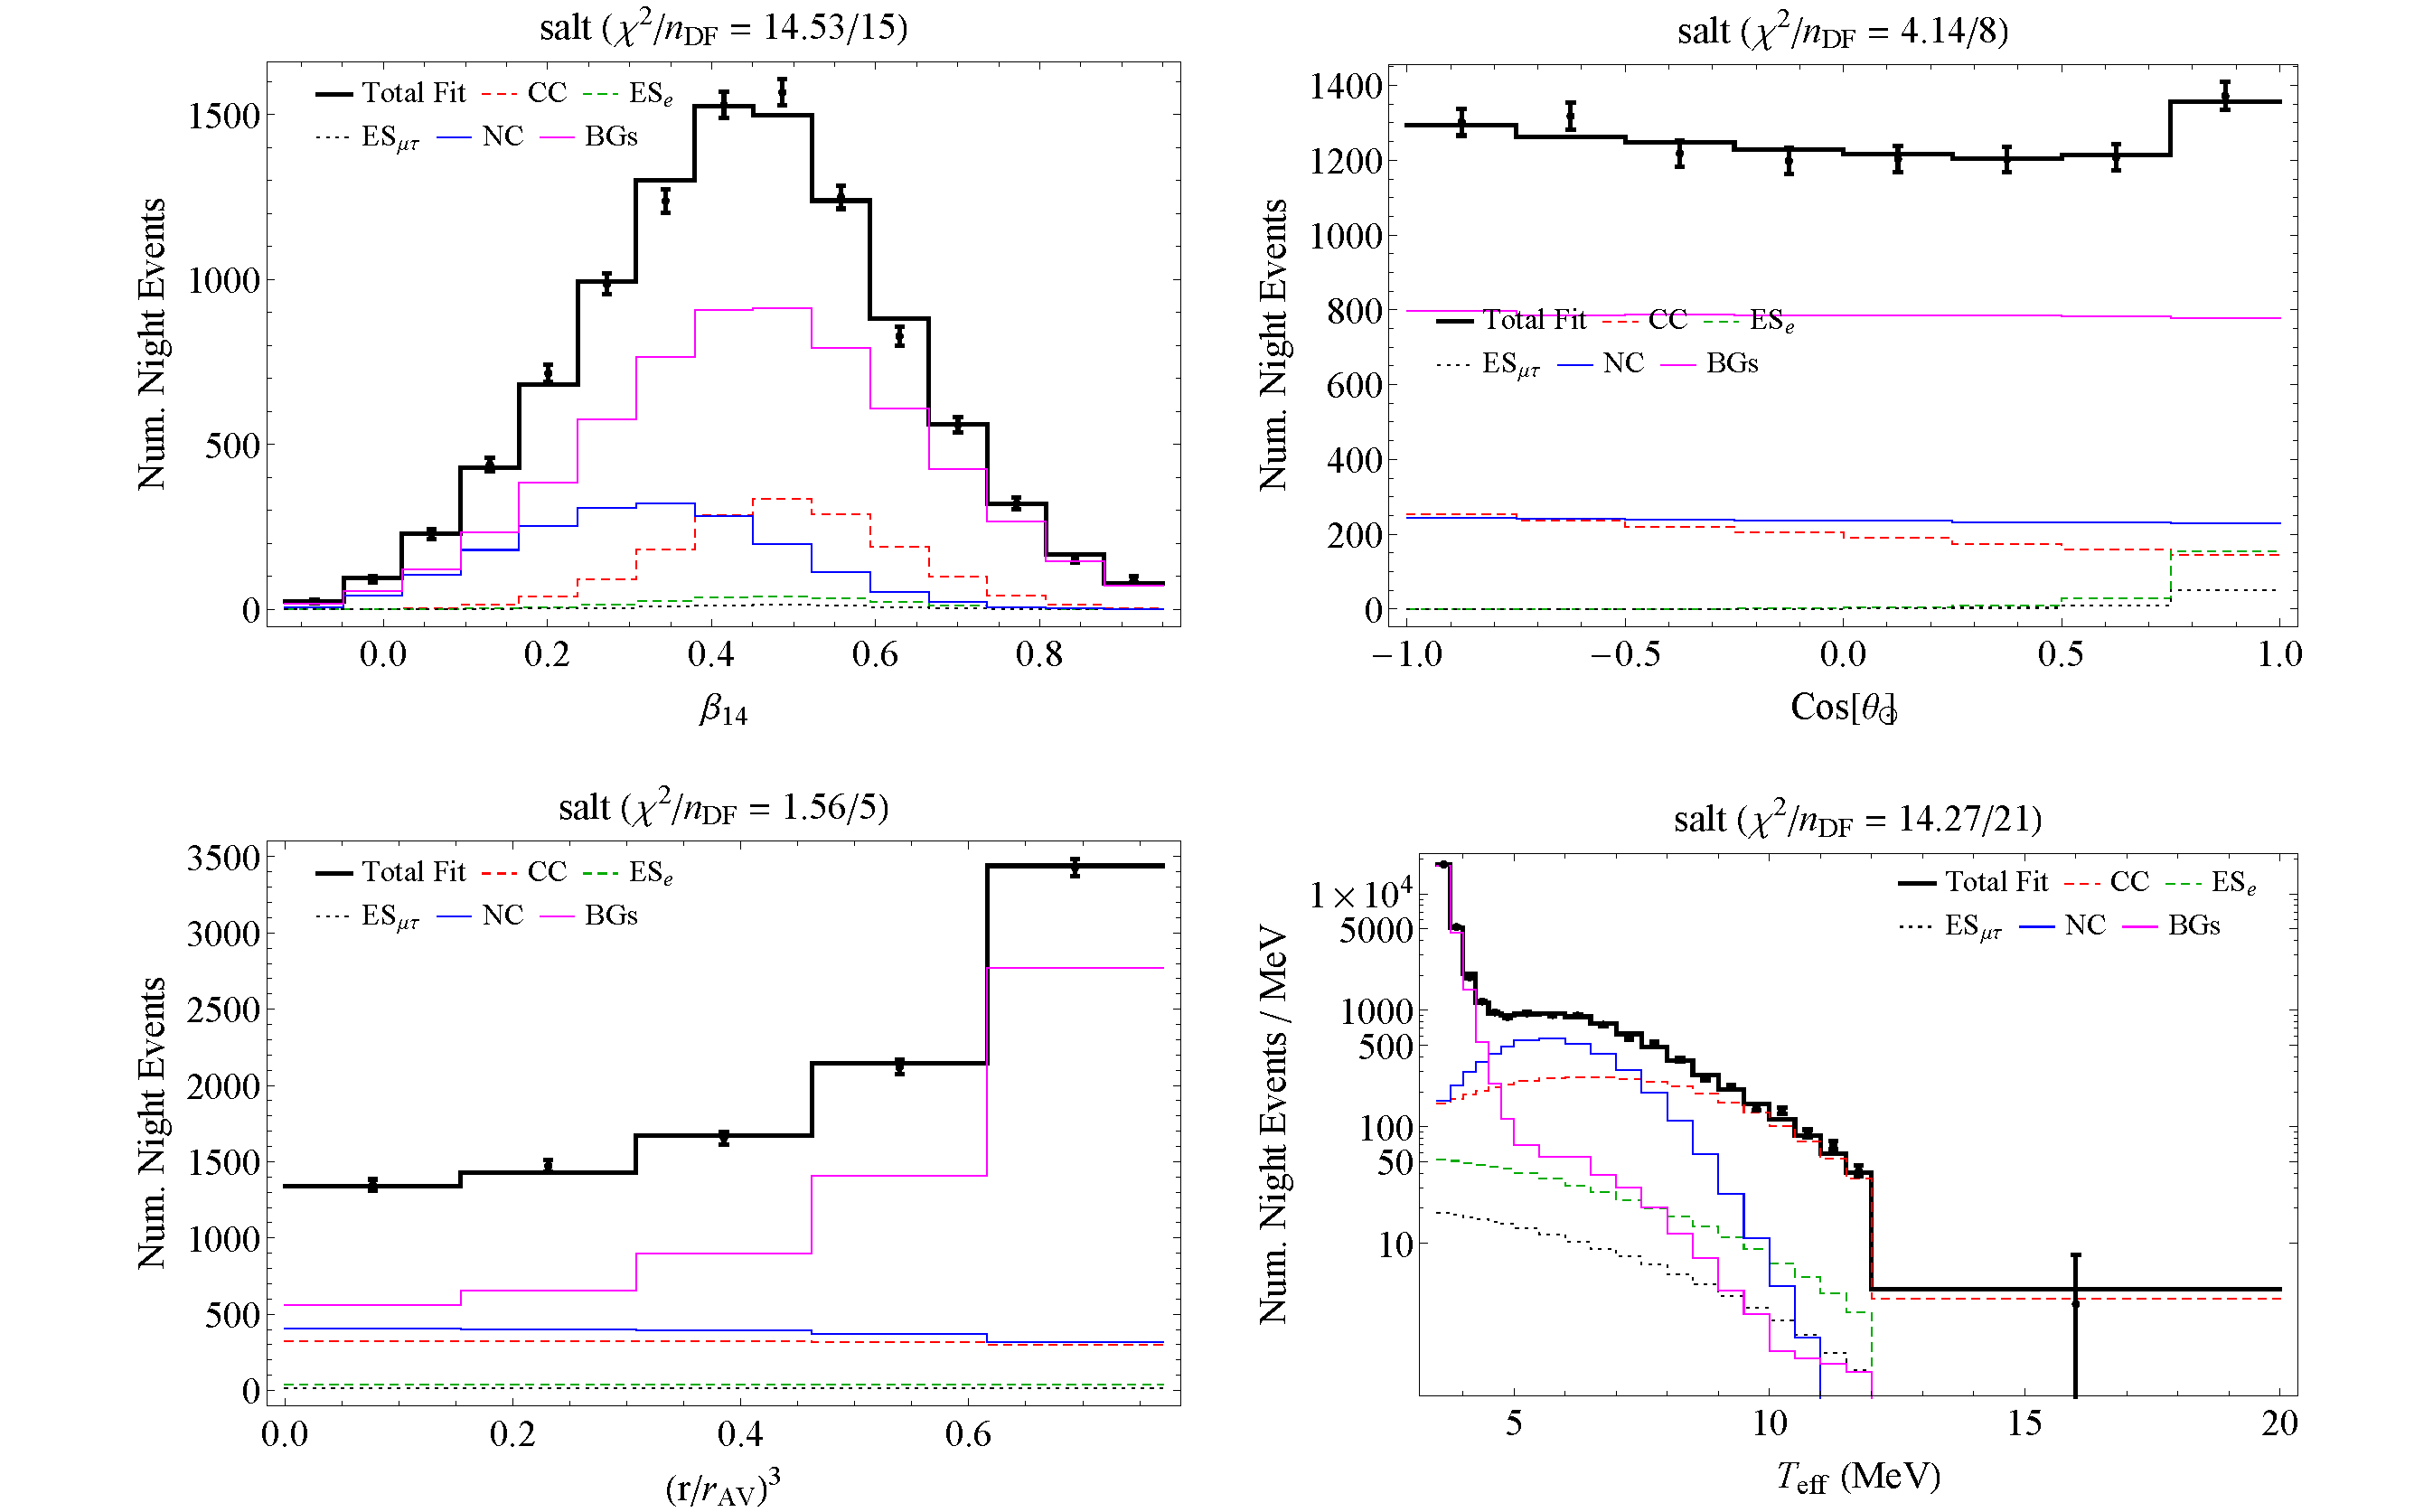
\includegraphics[width=0.95\columnwidth]{final_inf_salt_night}
\caption{\label{fig:final_inf_salt_obs}Observable distributions for Phase II for the final fit with $k_2$ fixed to infinity.}
\end{figure}
\begin{figure}
\centering
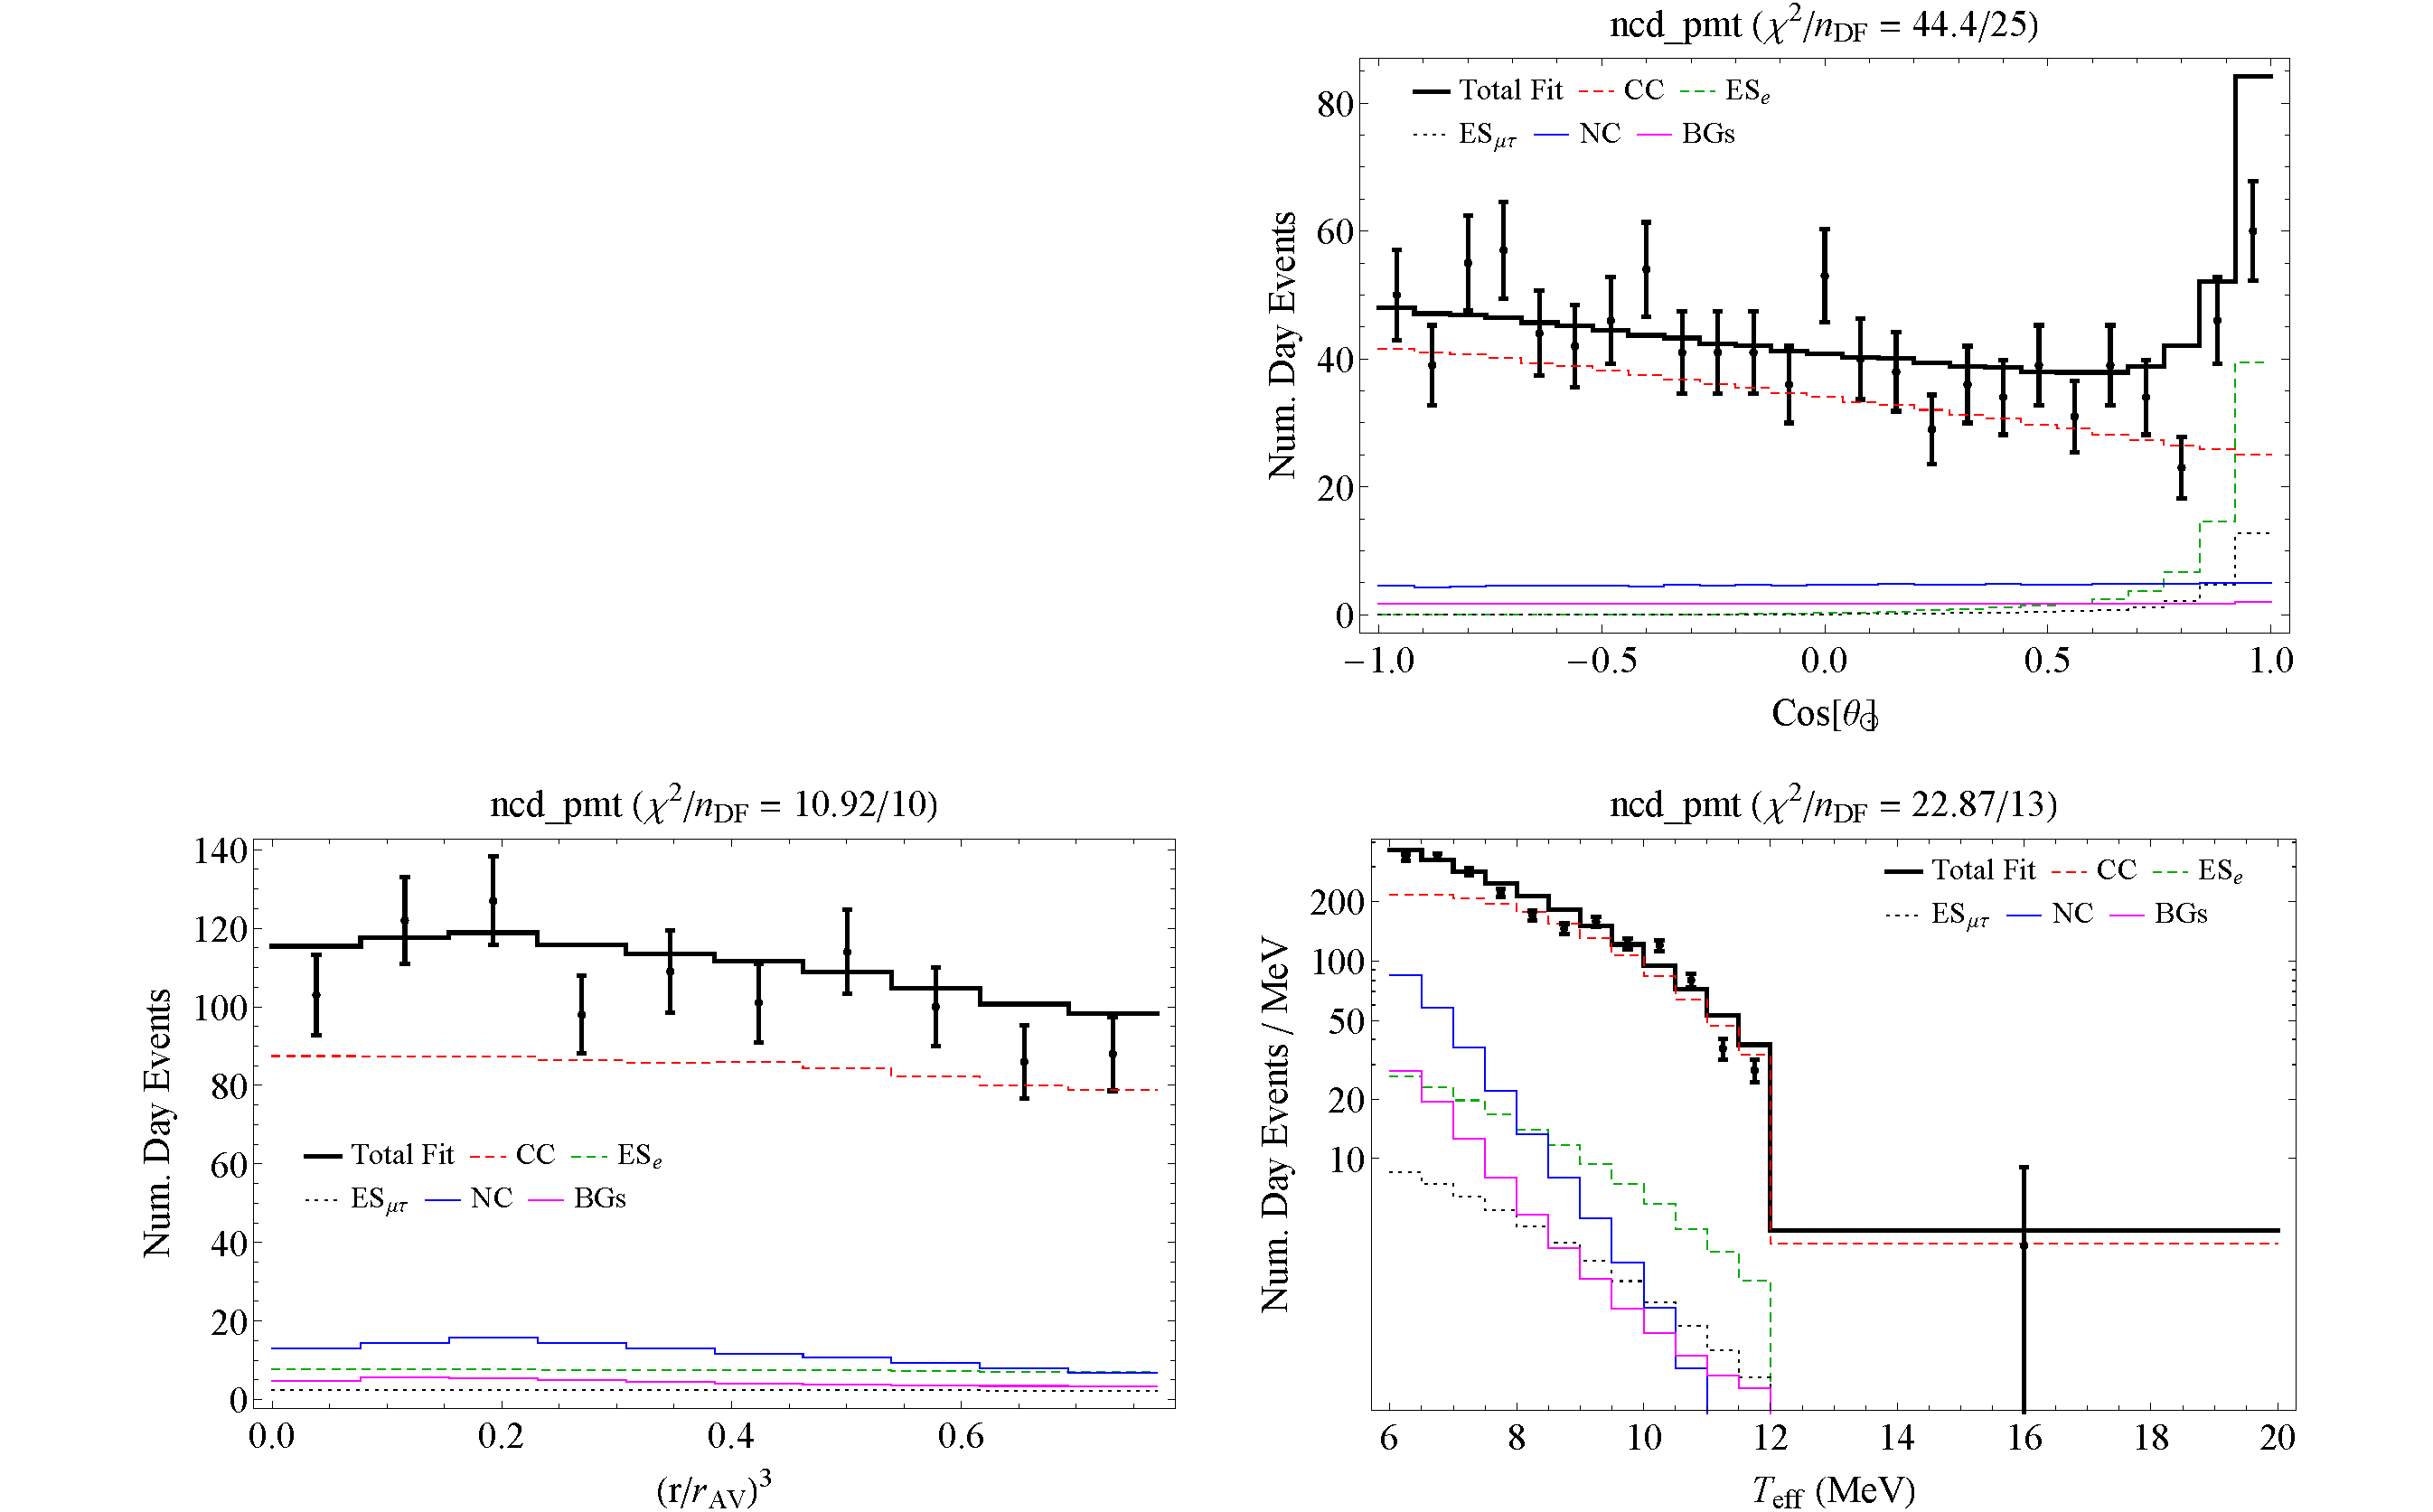
\includegraphics[width=0.95\columnwidth]{final_inf_ncd_pmt_day}
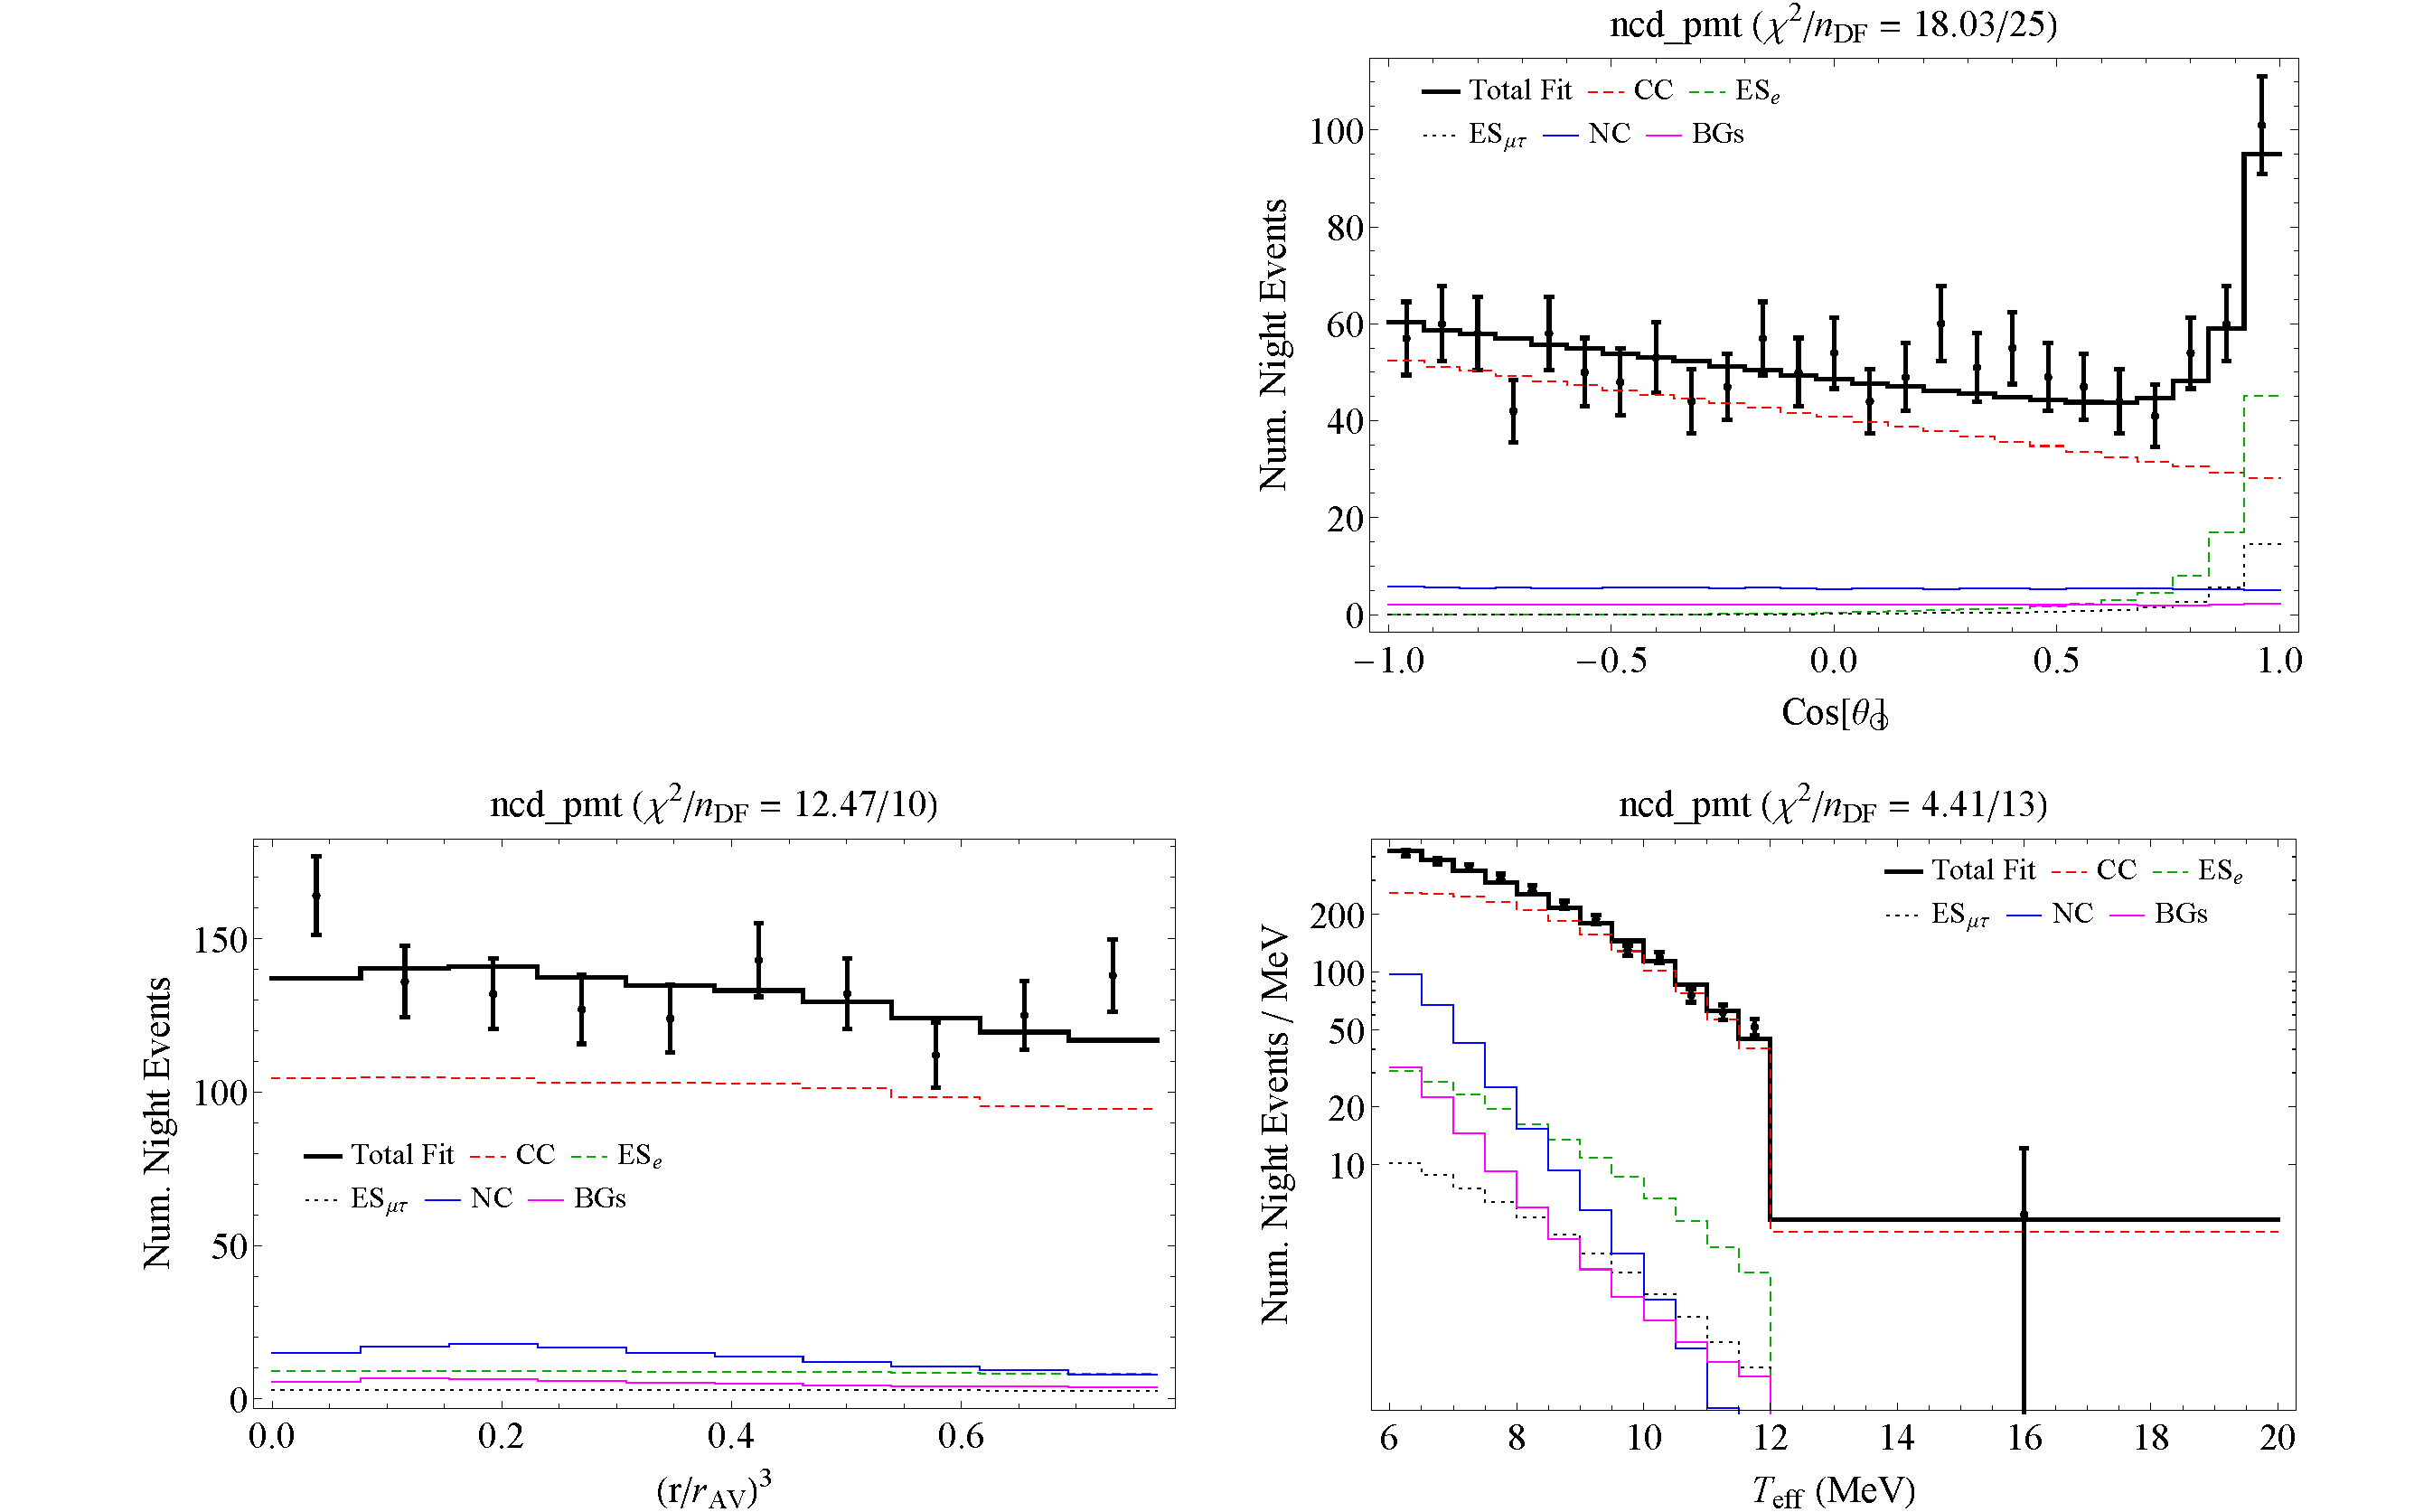
\includegraphics[width=0.95\columnwidth]{final_inf_ncd_pmt_night}
\caption{\label{fig:final_inf_ncd_pmt_obs}Observable distributions for Phase IIIb for the final fit with $k_2$ fixed to infinity. Note that $\beta_{14}$ was not used in analyses for NCD phase.}
\end{figure}
